\chapter{Experiments} \label{chap:experiments}

\minitoc \mtcskip \noindent

The developed framework presented and described in Chapter~\ref{chap:framework} obligate us to the validation of each module in order to assure consistency and robustness in the results that such system produced. Having this considered, we stipulate several experiments, in which each of them was related to a specific task. 

\section{Exploratory Data Analysis}\label{sec:exploratory_data_analysis}

The main goal of this section is the devise of relevant analysis taking into consideration the five different collected datasets. Since this dissertation is supported in experiments using real-world data, such analysis is crucial in order to gain better knowledge of the intrinsic characteristics of it. A tweet provides some fields of interest, such as, the text message, date of creation, language, and the \emph{entities}, which are constantly analysed in several data analytics systems. An \emph{entity} is metadata and additional contextual information contained in the tweet and is composed by the \emph{hashtags}, \emph{user mentions}, \emph{urls} and \emph{media} fields. We count the amount of tweets containing this kind of information for all the cities, London, New York, Melbourne, Rio de Janeiro and São Paulo, and projected some data visualizations for different temporal frequencies. The following subsections are divided into three different categories:  (1) Geographical Distribution, (2) Temporal Frequencies and (3) Metadata Composition. Additionally, we discuss the results of each city, as well as the main observable differences.

\subsection{Geographic Distributions}\label{subsec:geographical_distribution}

As previously mentioned, in Section~\ref{sec:data_collection}, we exploit an auxiliary \textit{online} tool to generate the coordinates for the bounding-boxes used in the collection process. The visual representation of the each city bounding-box is illustrated in Figure~\ref{fig:bounding_boxes}, as well as its the corresponding coordinates which are presented in Table~\ref{tab:bbs_points}.

\begin{figure}[t]
	\centering
	\begin{subfigure}[t]{0.31\textwidth}
		\centering
		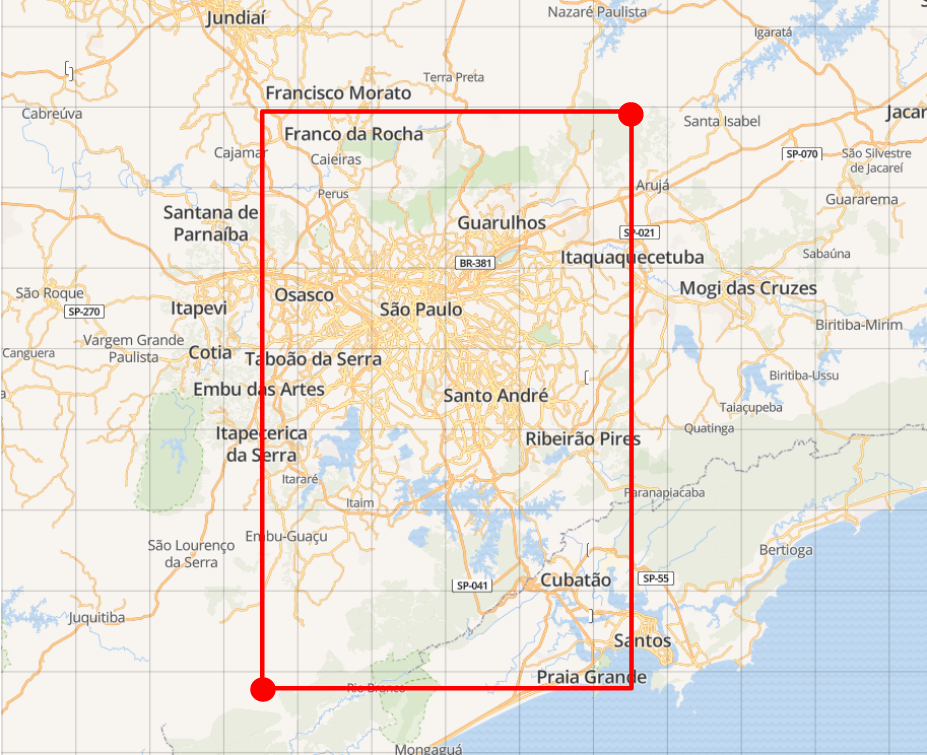
\includegraphics[width=1\linewidth]{figures/sp_bb.png}
		\caption{São Paulo}
		\label{fig:saopaulo_bounding_box}
	\end{subfigure}%
	\quad
	\begin{subfigure}[t]{0.3\textwidth}
		\centering
		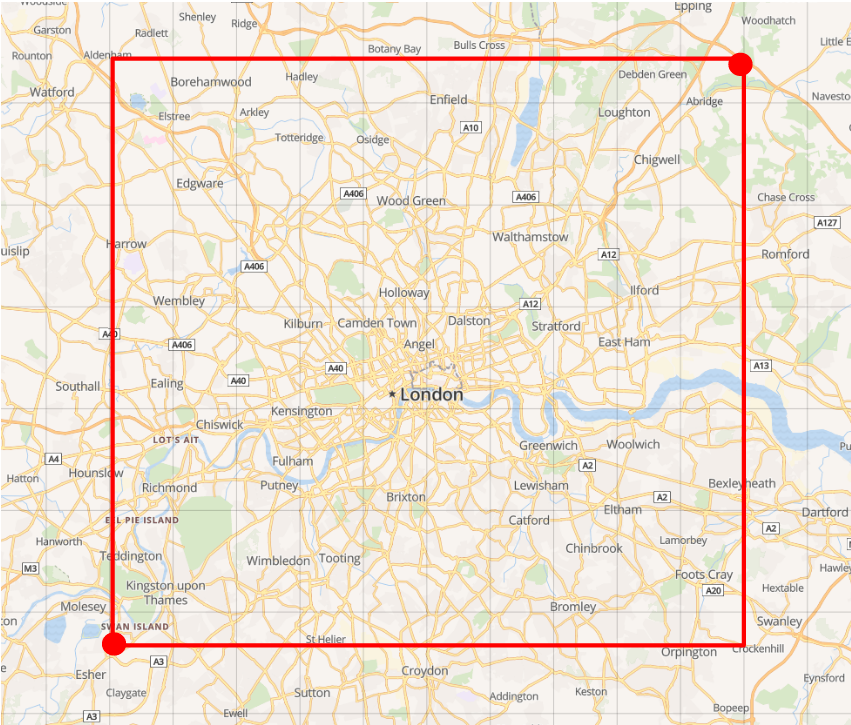
\includegraphics[width=1\linewidth]{figures/london_bb.png}
		\caption{London}
		\label{fig:london_bounding_box}
	\end{subfigure}
	\quad
	\begin{subfigure}[t]{0.3\textwidth}
		\centering
		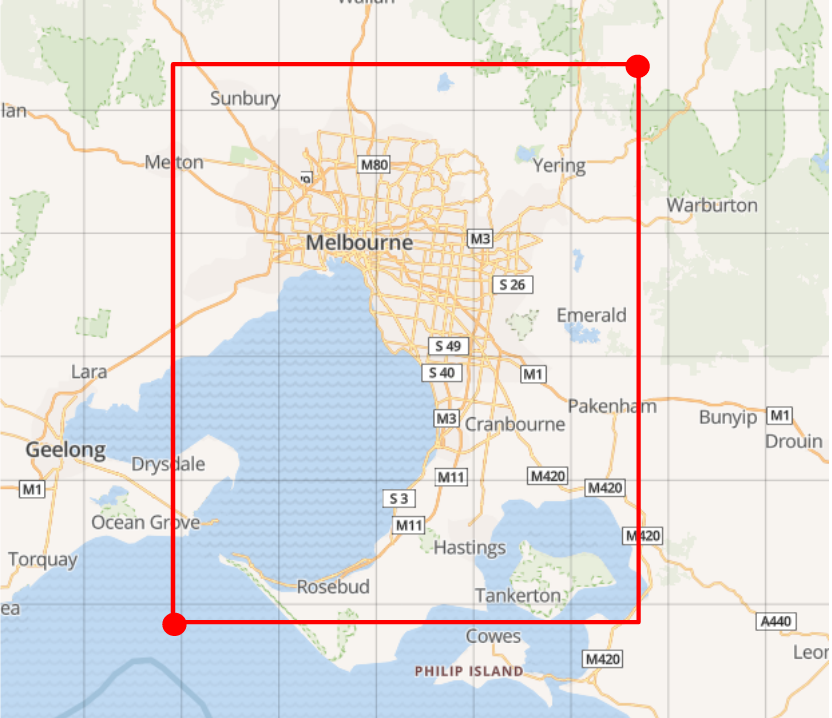
\includegraphics[width=1\linewidth]{figures/melbourne_bb.png}
		\caption{Melbourne}
		\label{fig:melbourne_bounding_box}
	\end{subfigure}
	
	\medskip
	
	\begin{subfigure}[t]{0.42\textwidth}
		\centering
		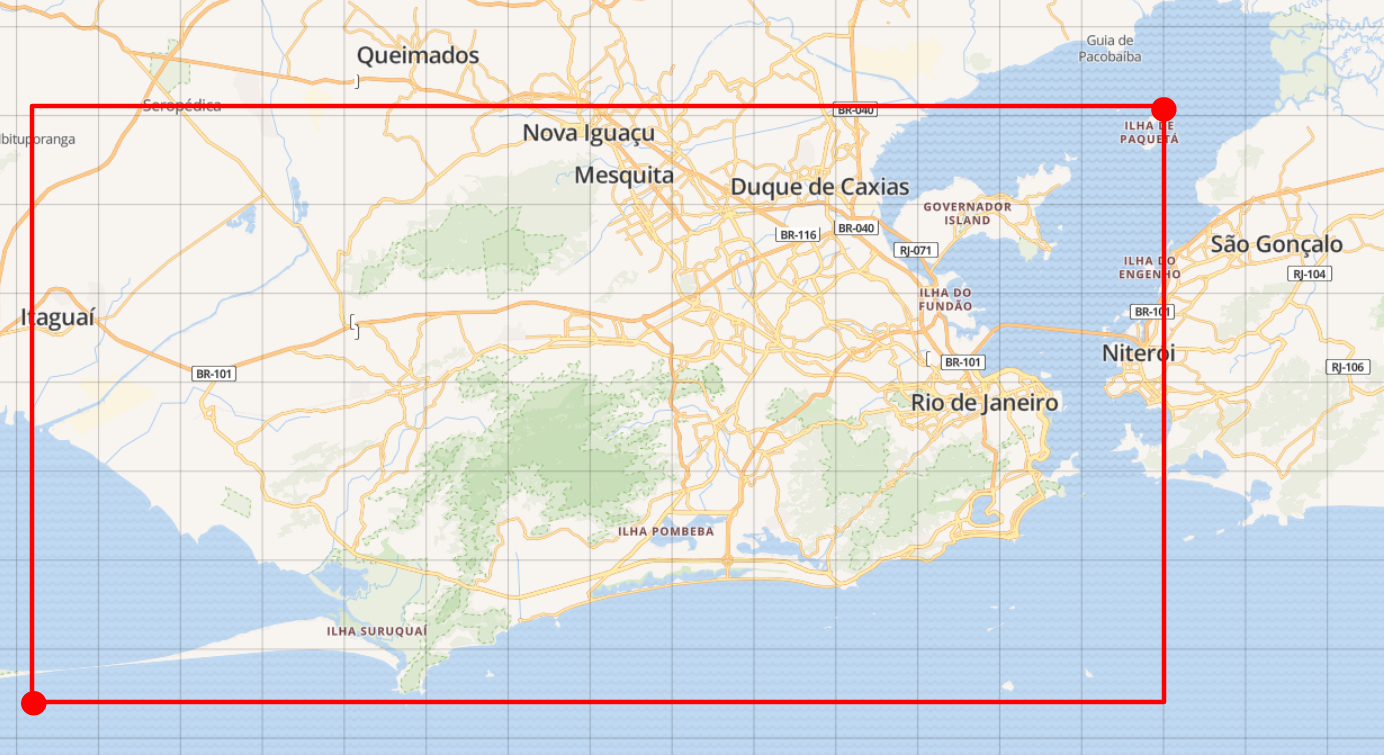
\includegraphics[width=1\linewidth]{figures/rio_bb.png}
		\caption{Rio de Janeiro}
		\label{fig:riodejaneiro_bounding_box}
	\end{subfigure}
	\quad
	\begin{subfigure}[t]{0.38\textwidth}
		\centering
		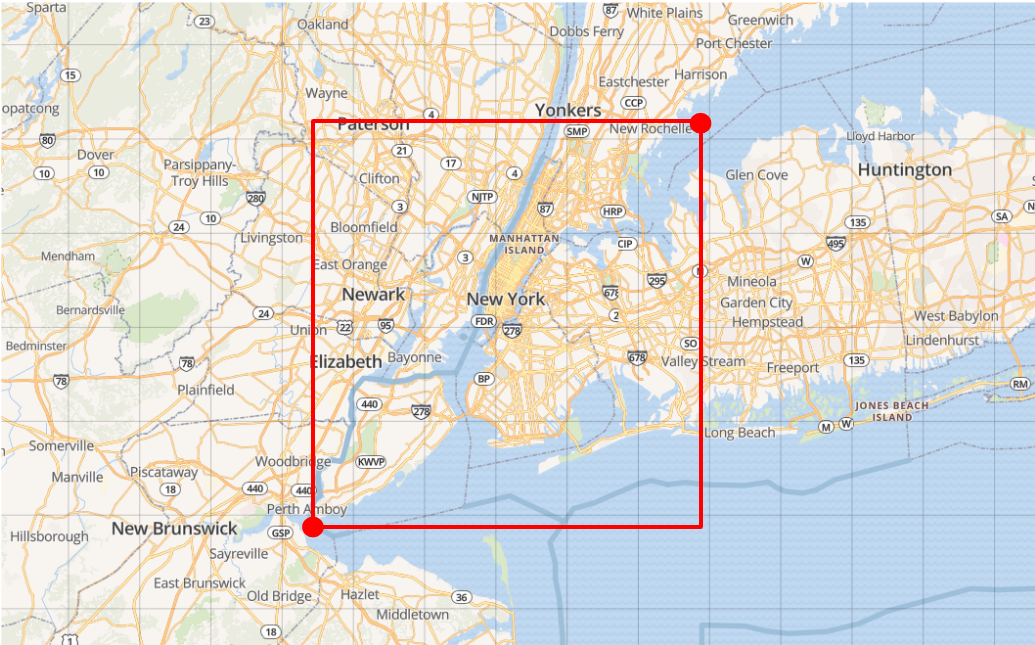
\includegraphics[width=1\linewidth]{figures/newyork_bb.png}
		\caption{New York}
		\label{fig:newyork_bounding_box}
	\end{subfigure}
	\caption{Search Bounding-boxes for the data collection}
	\label{fig:bounding_boxes}
\end{figure}

\begin{table}[b]
	\centering
	\setlength\extrarowheight{3pt}
	\caption{Collecting Bounding-boxes Coordinates (South-West and North-East)}
	\label{tab:bbs_points}
	\begin{tabular}{l|c|c}
		\hline
		\multicolumn{1}{c|}{\textbf{City}} & \textbf{South-West} & \textbf{North-East} \\ \hline
		\textbf{Rio de Janeiro} & (-43.7950599, -23.0822288) & (-43.0969042, -22.7460327) \\
		\textbf{São Paulo} & (-46.825514, -24.0082209) & (-46.3650844, -23.3566039) \\
		\textbf{New York City} & (-74.2590899, 40.4773991) & (-73.7002721, 40.9175771) \\
		\textbf{London} & (-0.3514683, 51.3849401) & (0.148271, 51.6723432) \\
		\textbf{Melbourne} & (144.5937418, -38.4338593) & (145.5125288, -37.5112737) \\ \hline
	\end{tabular}
\end{table}

Taking a careful observation into to coordinates used to each bounding-box, we can affirm that Rio de Janeiro present the broadest bounding-box comparatively to the others cities.

In the first attempts to study the geographic distribution in our datasets, we discover that not all tweets had a precise coordinate attached to it. Nonetheless, there were cases where tweets from other cities were collected to our datasets and this phenomenon is not supposed to happen when the collection method is based in geo-located characteristics. By studying the Twitter mobile application, we found out that a user can tag himself in the tweet by two different ways: (1) a user can activate the GPS in the mobile application and associate to the tweet his precisely geo-location; (2) a user can choose a place from a predefined list provide by Twitter and associate the place to the tweet.

The second method of tagging the geo-location to the tweet can arise some conflicts when this kind of tweets is used to perform scientific studies or even development of system to help the cities in the regularization, control and improvement of its services. Having this in consideration, it was necessary to understand how the Twitter Streaming API works and what kind of heuristics follows in order to retrieve this type of tweets. Hence, the documentation~\footnote{\url{https://dev.twitter.com/streaming/overview/request-parameters\#locations} (last visited on 17 June, 2017)} enhances two different heuristics:

\begin{enumerate}
	\item If the coordinates field is populated, the values there will be tested against the bounding-box;
	\item If the coordinates field is empty but place is populated, the region defined in place is checked for intersections against the locations bounding-box. Any overlapping areas will yield a positive match.
\end{enumerate}

The first heuristic only happens if a user is able/willing to tag a post with his precise geo-location associated with it; otherwise, the user can tag the post associated with a place and in this case the second heuristic is applied. 
Each place contained in the previous mentioned list, which is provided by Twitter, is composed by a bounding-box, and if any piece of it overlaps the bounding-box used in the collecting process, then a positive match is yielded and the tweet is retrieved. For example, if a tweet has a place such as Brazil and our filter bounding-box is defined for Rio de Janeiro, all tweets from place Brazil will be in our dataset, regardless the fact some tweets are posted elsewhere, such as in the city of Manaus, very far away from Rio de Janeiro.

This restriction required the development of a external layer which was responsible for the filter of tweets located outside the area of each city. To built this so, it was necessary \textit{a posteriori} information and, thus, we extract the Twitter default bounding-box of each city appealing to the tweets \textit{place} field. Such information was then used as the limit area in order to filter out tweets which \textit{coordinates} field was not populated. These bounding-boxes, the Twitter default ones, are listed in Table~\ref{tab:bbs_filter} and its corresponding visualization is the biggest rectangle demonstrated in Figures~\ref{fig:rio_sp_geographical_distribution} (subfigures~\ref{subfig:riodejaneiro_bounding_boxes} and~\ref{subfig:saopaulo_bounding_boxes}) and~\ref{fig:nyc_london_melbourne_geographical_distribution} (subfigures~\ref{subfig:nyc_bounding_boxes},~\ref{subfig:london_bounding_boxes} and~\ref{subfig:melbourne_bounding_boxes}).

\begin{table}[htbp]
	\centering
	\setlength\extrarowheight{3pt}
	\caption{Twitter Default Bounding-boxes Coordinates (South-West and North-East)}
	\label{tab:bbs_filter}
	\begin{tabular}{l|c|c}
		\hline
		\multicolumn{1}{c|}{\textbf{City}} & \textbf{South-West} & \textbf{North-East} \\ \hline
		\textbf{Rio de Janeiro} & (-43.795449, -23.08302) & (-43.087707, -22.739823) \\
		\textbf{São Paulo} & (-46.826039, -24.008814) & (-46.365052, -23.356792) \\
		\textbf{New York City} & (-74.255641, 40.495865) & (-73.699793, 40.91533) \\
		\textbf{London} & (-0.510365, 51.286702) & (0.334043, 51.691824) \\
		\textbf{Melbourne} & (144.593742, -38.433859) & (145.512529, -37.511274) \\ \hline
	\end{tabular}
\end{table}

The final volume of tweets located inside and outside the cities correspondent bounding-boxes are presented in Table~\ref{tab:geographic_counts_bb}. Alongside with the location analysis, the language count was also performed since future experiments only took into consideration tweets with the native language of the city in study and not foreign ones. In the abovementioned table (\ref{tab:geographic_counts_bb}) it is possible to verify a vast difference regarding the activity on Twitter in Rio de Janeiro. Numbers tell that such activity, with respect to geo-located tweets, is almost two times more than São Paulo, four times London and twenty five times Melbourne. A possible justification for this noticeable difference may be associated to the area of the bounding-box used in the collection process, but, on the other hand, according to some sources related to the demographic measures, for the case Rio De Janeiro \textit{versus} São Paulo, the population volume has an opposite behavior, where São Paulo~\footnote{\url{https://cidades.ibge.gov.br/v4/brasil/sp/sao-paulo/panorama} (last visited on 17 June, 2017)} has almost 12 millions habitants while Rio de Janeiro~\footnote{\url{https://cidades.ibge.gov.br/v4/brasil/rj/rio-de-janeiro/panorama} (last visited on 17 June, 2017)} has 6 million. Having only this amount of information it is impossible, at the moment, formulate a explanation to this phenomenon.

\begin{table}[htbp]
	\centering
	\caption{Datasets composition after verification of the tweets inside the corresponding bounding-box}
	\label{tab:geographic_counts_bb}
	\resizebox{\textwidth}{!}{\begin{tabular}{l|c|cl|cl|cl|cl|cl}
			\hline
			\multicolumn{1}{c|}{\multirow{2}{*}{\textbf{City}}} & \multirow{2}{*}{\textbf{All}} & \multicolumn{2}{c|}{\textbf{PT/EN}} & \multicolumn{2}{c|}{\textbf{Non-PT/EN}} & \multicolumn{2}{c|}{\textbf{\begin{tabular}[c]{@{}c@{}}In\\ Bounding-Box\end{tabular}}} & \multicolumn{2}{c|}{\textbf{\begin{tabular}[c]{@{}c@{}}Out\\ Bounding-Box\end{tabular}}} & \multicolumn{2}{c|}{\textbf{\begin{tabular}[c]{@{}c@{}}PT/EN and In\\ Bounding-Box\end{tabular}}} \\ \cline{3-12} 
			\multicolumn{1}{c|}{} &  & \textbf{No. tweets} & \multicolumn{1}{c|}{\textbf{\%}} & \textbf{No. tweets} & \multicolumn{1}{c|}{\textbf{\%}} & \textbf{No. tweets} & \multicolumn{1}{c|}{\textbf{\%}} & \textbf{No. tweets} & \multicolumn{1}{c|}{\textbf{\%}} & \textbf{No. tweets} & \multicolumn{1}{c}{\textbf{\%}} \\ \hline
			\textbf{Rio de Janeiro} & 18,803,774 & 15,906,680 & 84,59\% & 2,897,094 & 15,41\% & 12,976,048 & 69,01\% & 5,827,726 & 30,99\% & 11,060,136 & 58,82\% \\
			\textbf{São Paulo} & 9,319,624 & 7,203,115 & 77,29\% & 2,116,509 & 22,71\% & 6,237,427 & 66,93\% & 3,082,197 & 33,07\% & 4,886,626 & 52,43\% \\
			\textbf{New York City} & 8,507,145 & 7,260,829 & 85,35\% & 1,246,316 & 14,65\% & 6,972,312 & 81,96\% & 1,534,833 & 18,04\% & 5,956,355 & 70,02\% \\
			\textbf{London} & 5,596,551 & 4,774,310 & 85,31\% & 822,241 & 14,69\% & 4,752,918 & 84,93\% & 843,633 & 15,07\% & 4,040,092 & 72,19\% \\
			\textbf{Melbourne} & 789,927 & 669,435 & 84,75\% & 120,492 & 15,25\% & 742,946 & 94,05\% & 46,981 & 5,95\% & 629,424 & 79,68\% \\ \hline
		\end{tabular}}
	\end{table}

Later, after the filtering process, we tried to understand the volume, as well as the location of each tweet. Through this kind of analysis it was possible to find out that a tweet which \textit{coordinates }field was empty and is, actually, represented with a bounding-box, can also be a specific place, i.e. a place that has a precise coordinate. Not all places were represented by a bounding-box in which each point that composed it are different. An example to that is \texttt{Estádio do Maracanã} which although being represented by a bounding-box, all four points are equal. A division was made considering this three types of location - (1) bounding-box with four different points; (2) bounding-box with four equal points; (3) precise coordinate - in order to have a perception of how different specific places and bounding-boxes as so which is the volume of tweets that are related to it.

\begin{table}[htbp]
	\centering
	\caption{Volume of tweets for each type of geo-location}
	\label{tab:volume_geolocation}
	\resizebox{\textwidth}{!}{\begin{tabular}{l|c|ccc|ccc|ccc}
			\hline
			\multicolumn{1}{c|}{\multirow{2}{*}{\textbf{City}}} & \multirow{2}{*}{\textbf{Total}} & \multicolumn{3}{c|}{\textbf{Bounding-boxes}} & \multicolumn{3}{c|}{\textbf{Specific Places}} & \multicolumn{3}{c|}{\textbf{Precisely}} \\ \cline{3-11} 
			\multicolumn{1}{c|}{} &  & \multicolumn{1}{c|}{\textbf{Distinct}} & \multicolumn{1}{c|}{\textbf{No. Tweets}} & \textbf{Percentage (\%)} & \multicolumn{1}{c|}{\textbf{Distinct}} & \multicolumn{1}{c|}{\textbf{No. Tweets}} & \textbf{Percentage (\%)} & \multicolumn{1}{c|}{\textbf{Distinct}} & \multicolumn{1}{c|}{\textbf{No. Tweets}} & \textbf{Percentage (\%)} \\ \hline
			\textbf{Rio de Janeiro} & 11060136 & 297 & 10237280 & 92,56\% & 11159 & 49440 & 0,45\% & 163748 & 773416 & 6,99\% \\
			\textbf{São Paulo} & 4886626 & 325 & 4284795 & 87,68\% & 7189 & 21022 & 0,43\% & 100028 & 580809 & 11,89\% \\
			\textbf{New York City} & 5956355 & 328 & 4210854 & 70,70\% & 16078 & 85204 & 1,43\% & 138123 & 1660297 & 27,87\% \\
			\textbf{London} & 4040092 & 53 & 3196043 & 79,11\% & 8123 & 53412 & 1,32\% & 95317 & 790637 & 19,57\% \\
			\textbf{Melbourne} & 629424 & 22 & 523870 & 83,23\% & 0 & 0 & 0,00\% & 21826 & 105554 & 16,77\% \\ \hline
		\end{tabular}}
	\end{table}
	
The final counts of the analysis for each identified type of geo-location are presented in Table~\ref{tab:volume_geolocation}. Looking at the numbers it is possible to conclude some facts applicable to all cities. Citizens tend to geo-locate themselves with a location which has variable bounding-box size since more than 70\% of the tweets are of this type. Furthermore, only a few percentage of tweets, between 0\% and 1.43\%, are located in specific places, although the existence of a higher number of distinct specific places comparatively to the bounding-boxes with variable size, with exception of Melbourne that has zero specific places in our dataset. Other interesting point to enhance is the considerable percentage of tweets with precise location (i.e. tweets that people tagged himself using the GPS). The Brazilian cities proved to be less supportive of precisely located tweets, while the English cities were more contributive. The distribution of each type of geo-located tweet is illustrated in Figures~\ref{fig:rio_sp_geographical_distribution} and~\ref{fig:nyc_london_melbourne_geographical_distribution}. The variable bounding-boxes are showed in ~\ref{subfig:saopaulo_bounding_boxes},~\ref{subfig:riodejaneiro_bounding_boxes},~\ref{subfig:nyc_bounding_boxes},~\ref{subfig:london_bounding_boxes} and~\ref{subfig:melbourne_bounding_boxes} proving that our filter method was able to correctly agglomerate places that were, indeed, inside of the Twitter default bounding-boxes. In~\ref{subfig:saopaulo_markers},~\ref{subfig:riodejaneiro_markers},~\ref{subfig:nyc_markers},~\ref{subfig:london_markers} and~\ref{subfig:melbourne_markers} is illustrated the distribution of the specific places found out in our datasets for each city. A particular point identified was the absence of specific places in Melbourne and the limited places in a certain area of London. With a first look at the image of London, there may be doubts about the results concerning the filter method, however the bounding-box used to that process was the same in both cases, and so the only viable explanation for such result is the absence of specific locations for that area in the predefined list of places provided by the Twitter applications. Lastly, in~\ref{subfig:saopaulo_points},~\ref{subfig:riodejaneiro_points},~\ref{subfig:nyc_points},~\ref{subfig:london_points} and~\ref{subfig:melbourne_points} is illustrated the distribution of precisely located tweets. Through a careful observation in this distribution it was possible the arising of another doubt relatively to the first aforementioned heuristic of the Twitter Streaming API. There were tweets retrieved that not matched the bounding-box used in the collection process and this fact conducts to uncertainty and mistrust regarding the performance of this type of collection available on Twitter. 

\begin{figure}[htbp]
	\centering
	\begin{subfigure}[htbp]{0.4\textwidth}
		\centering
		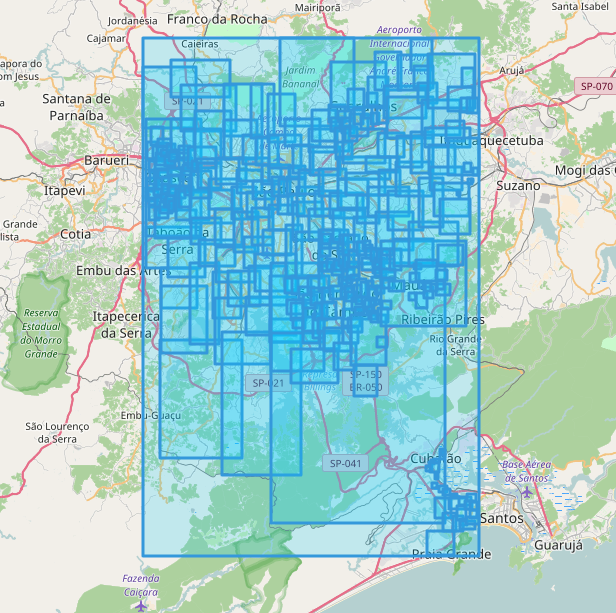
\includegraphics[width=1\linewidth]{figures/sp_bbs.png}
		\caption{}
		\label{subfig:saopaulo_bounding_boxes}
	\end{subfigure}
	\quad
	\begin{subfigure}[htbp]{0.5\textwidth}
		\centering
		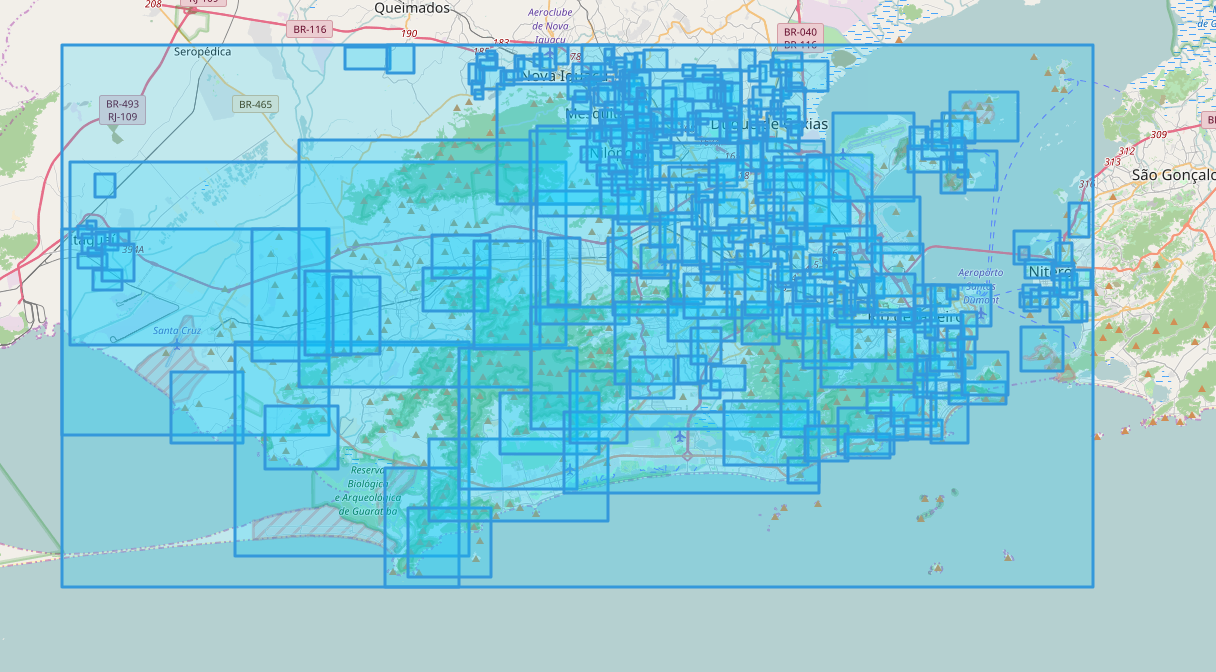
\includegraphics[width=1\linewidth]{figures/rio_bbs.png}
		\caption{}
		\label{subfig:riodejaneiro_bounding_boxes}
	\end{subfigure}
	
	\medskip
	
	\begin{subfigure}[htbp]{0.4\textwidth}
		\centering
		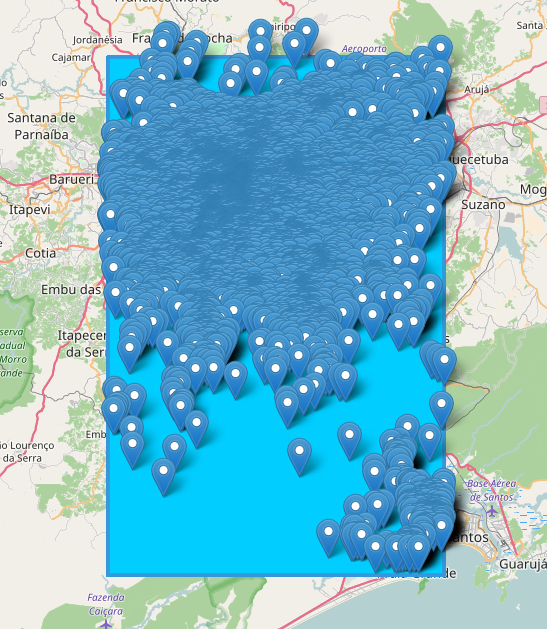
\includegraphics[width=1\linewidth]{figures/sp_markers.png}
		\caption{}
		\label{subfig:saopaulo_markers}
	\end{subfigure}
	\quad
		\begin{subfigure}[htbp]{0.5\textwidth}
			\centering
			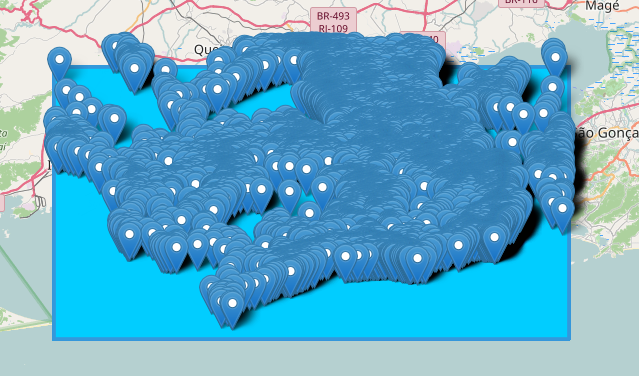
\includegraphics[width=1\linewidth]{figures/rio_markers.png}
			\caption{}
			\label{subfig:riodejaneiro_markers}
		\end{subfigure}
		
	\medskip
	
	\begin{subfigure}[htbp]{0.4\textwidth}
		\centering
		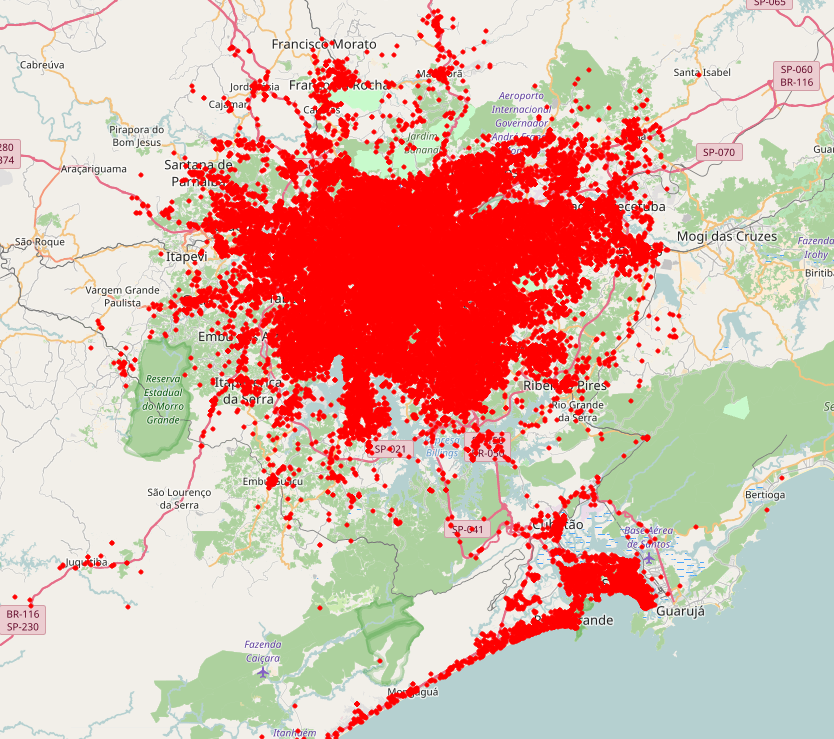
\includegraphics[width=1\linewidth]{figures/sp_points.png}
		\caption{}
		\label{subfig:saopaulo_points}
	\end{subfigure}
	\quad
	\begin{subfigure}[htbp]{0.5\textwidth}
		\centering
		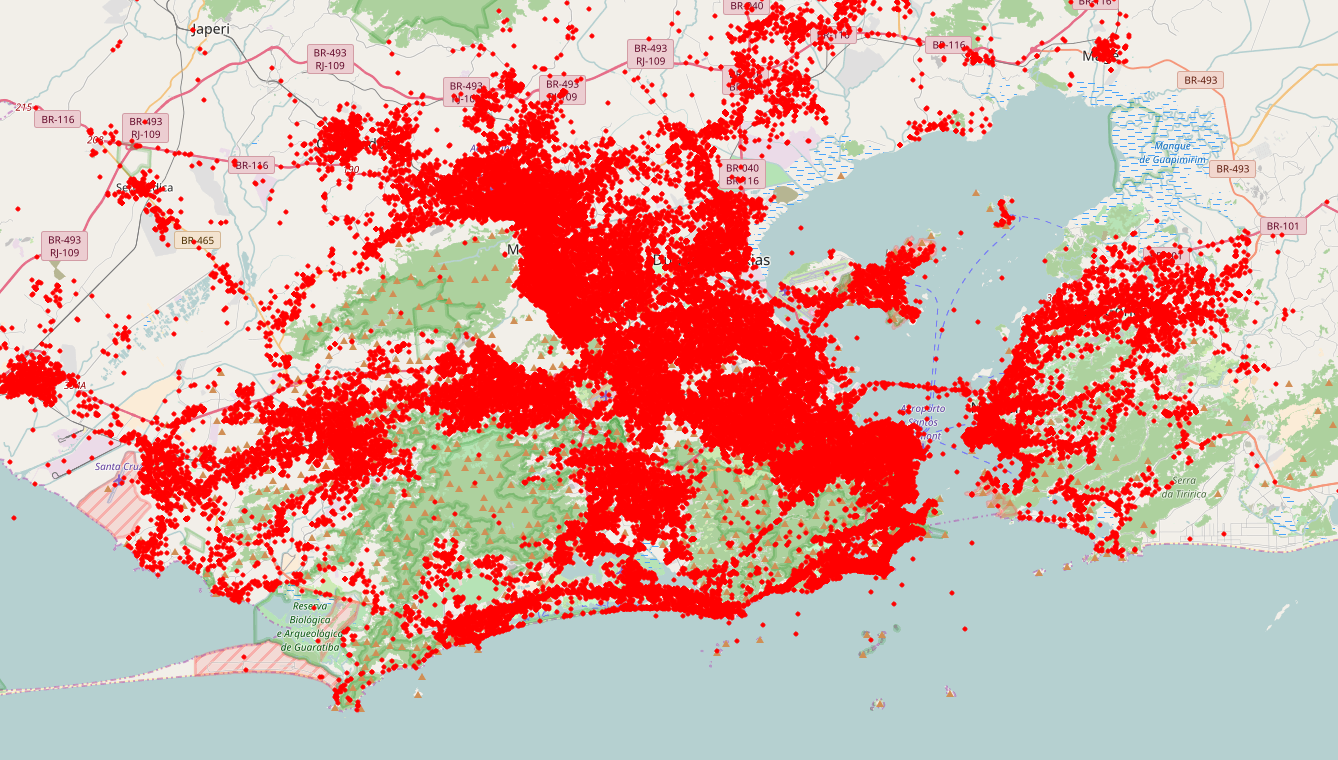
\includegraphics[width=1\linewidth]{figures/rio_points.png}
		\caption{}
		\label{subfig:riodejaneiro_points}
	\end{subfigure}
	
	\caption[Three numerical solutions]{São Paulo (a, c, e) and Rio de Janeiro (b, d, f) Geographical Distributions: (a, b) Bounding-boxes of places (c, d) Specific places (e, f) Geo-tagged tweets}
	\label{fig:rio_sp_geographical_distribution}
\end{figure}

\begin{figure}[htbp]
	\centering
	\begin{subfigure}[htbp]{0.3\textwidth}
		\centering
		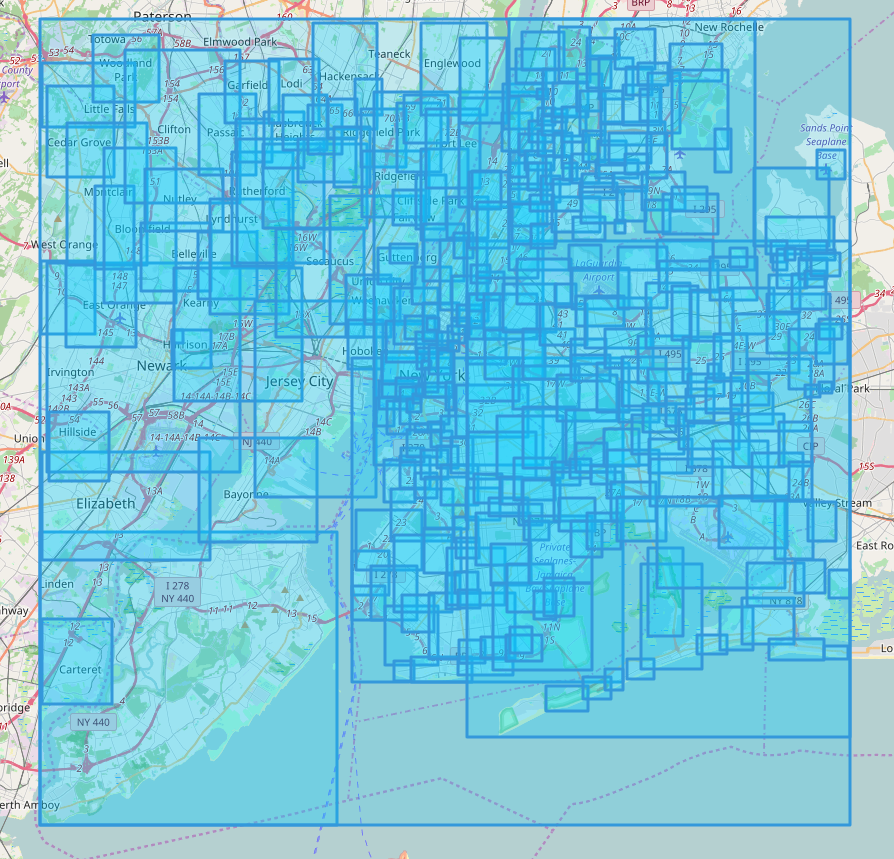
\includegraphics[width=1\linewidth]{figures/nyc_bbs.png}
		\caption{}
		\label{subfig:nyc_bounding_boxes}
	\end{subfigure}
	\quad
	\begin{subfigure}[htbp]{0.3\textwidth}
		\centering
		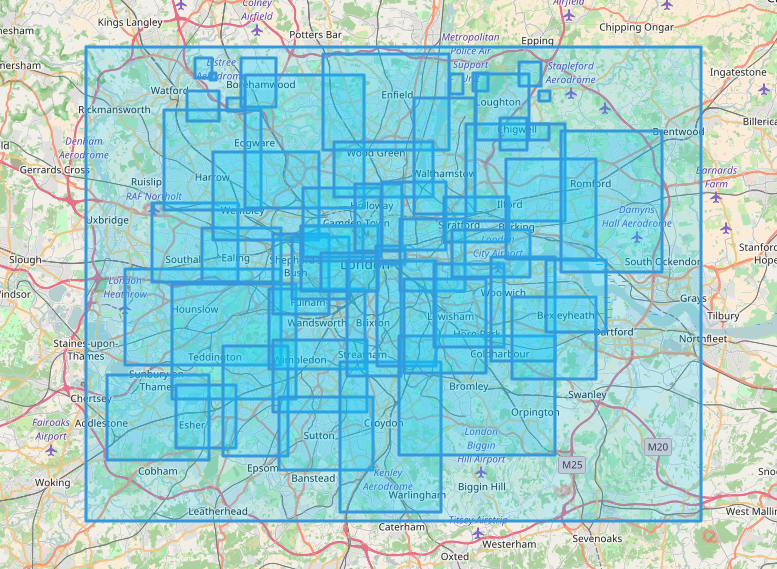
\includegraphics[width=1\linewidth]{figures/london_bbs.png}
		\caption{}
		\label{subfig:london_bounding_boxes}
	\end{subfigure}
	\quad
	\begin{subfigure}[htbp]{0.3\textwidth}
		\centering
		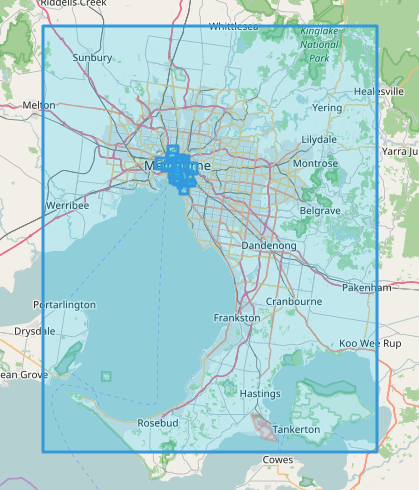
\includegraphics[width=1\linewidth]{figures/melbourne_bbs.png}
		\caption{}
		\label{subfig:melbourne_bounding_boxes}
	\end{subfigure}
			
	\medskip
	
	\centering
	\begin{subfigure}[htbp]{0.3\textwidth}
		\centering
		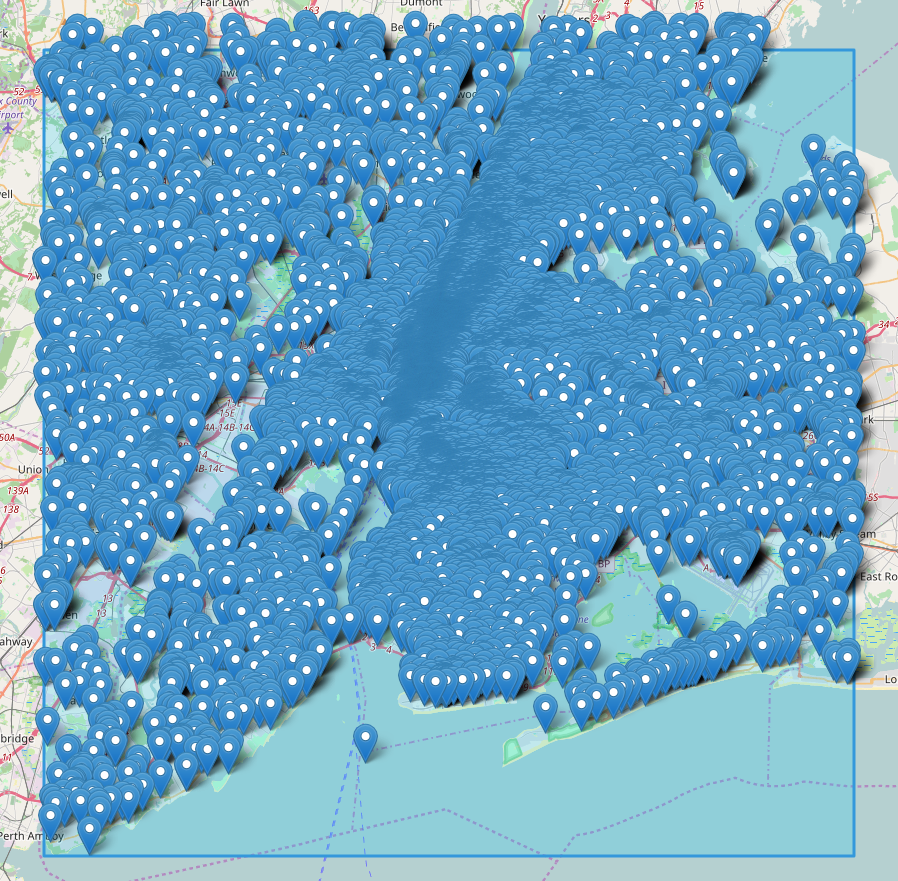
\includegraphics[width=1\linewidth]{figures/nyc_markers.png}
		\caption{}
		\label{subfig:nyc_markers}
	\end{subfigure}
	\quad
	\begin{subfigure}[htbp]{0.3\textwidth}
		\centering
		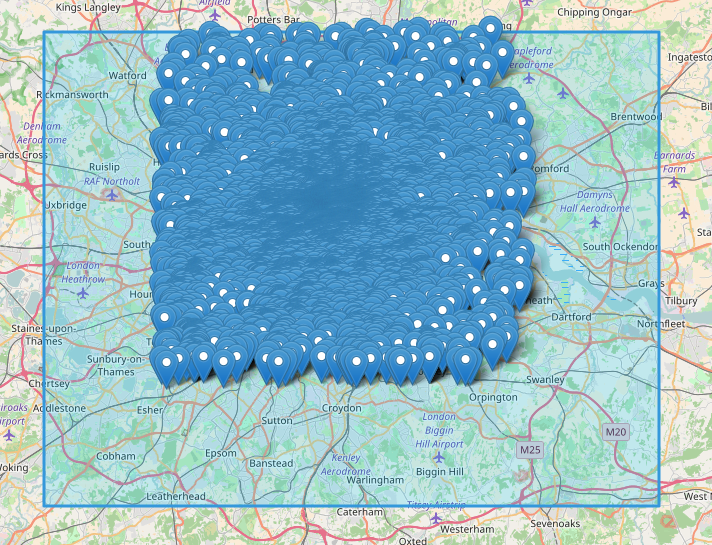
\includegraphics[width=1\linewidth]{figures/london_markers.png}
		\caption{}
		\label{subfig:london_markers}
	\end{subfigure}
	\quad
	\begin{subfigure}[htbp]{0.3\textwidth}
		\centering
		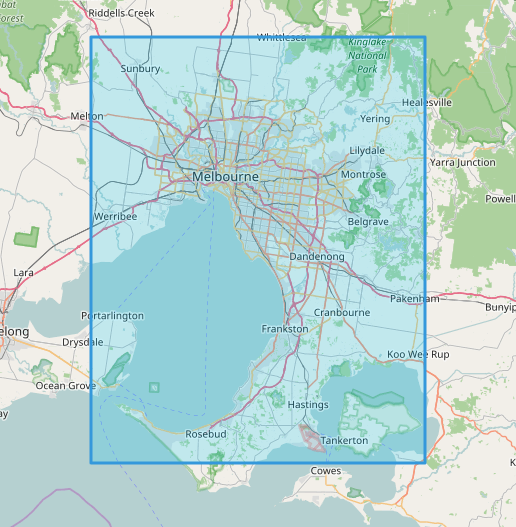
\includegraphics[width=1\linewidth]{figures/melbourne_markers.png}
		\caption{}
		\label{subfig:melbourne_markers}
	\end{subfigure}
	
	\medskip
	\centering
	\begin{subfigure}[htbp]{0.3\textwidth}
		\centering
		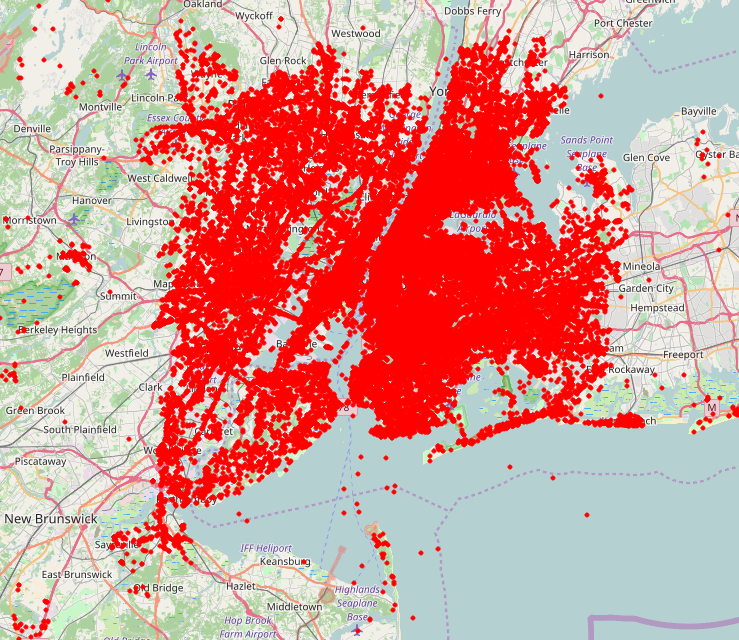
\includegraphics[width=1\linewidth]{figures/nyc_points.png}
		\caption{}
		\label{subfig:nyc_points}
	\end{subfigure}
	\quad
	\begin{subfigure}[htbp]{0.3\textwidth}
		\centering
		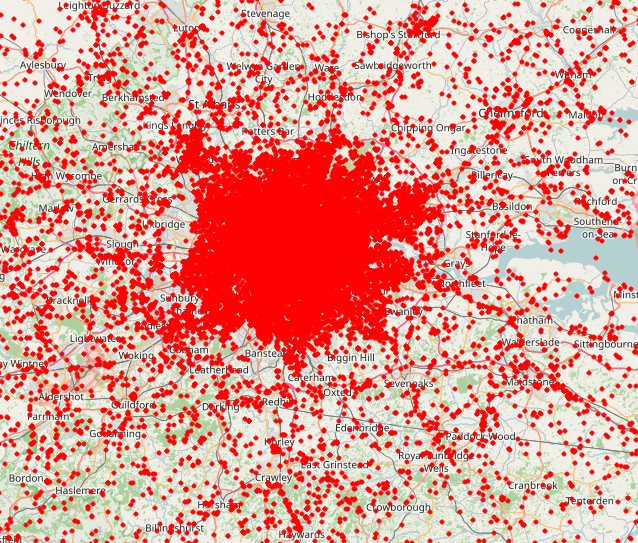
\includegraphics[width=1\linewidth]{figures/london_points.png}
		\caption{}
		\label{subfig:london_points}
	\end{subfigure}
	\quad
	\begin{subfigure}[htbp]{0.3\textwidth}
		\centering
		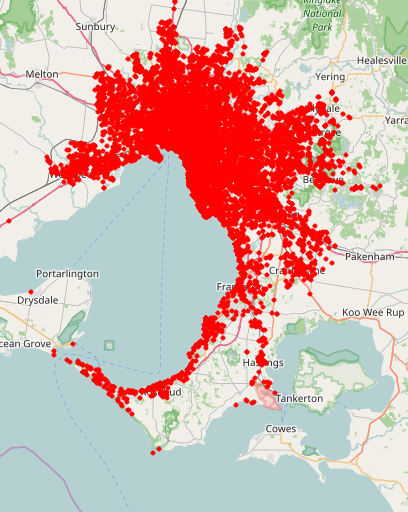
\includegraphics[width=1\linewidth]{figures/melbourne_points.png}
		\caption{}
		\label{subfig:melbourne_points}
	\end{subfigure}
	
	\caption[Three numerical solutions]{New York City (a, d, g), London (b, e, h) Geographical Distributions: (a, b) Bounding-boxes of places (c, d) Specific places (e, f) Geo-tagged tweets}
	\label{fig:nyc_london_melbourne_geographical_distribution}
\end{figure}

\subsection{Temporal Frequencies}

Another interesting analysis in our datasets concerns the temporal distribution of the data. The volume of tweets posted per hour, per day, as well as the activity by day-of-the-week or hour-of-the-day are statistics that enable the possibility of finding out patterns or variations which can be correlated to some events or incidents happening in a city.

\begin{figure}[htbp]
	\centering
	\begin{subfigure}[htbp]{0.8\textwidth}
		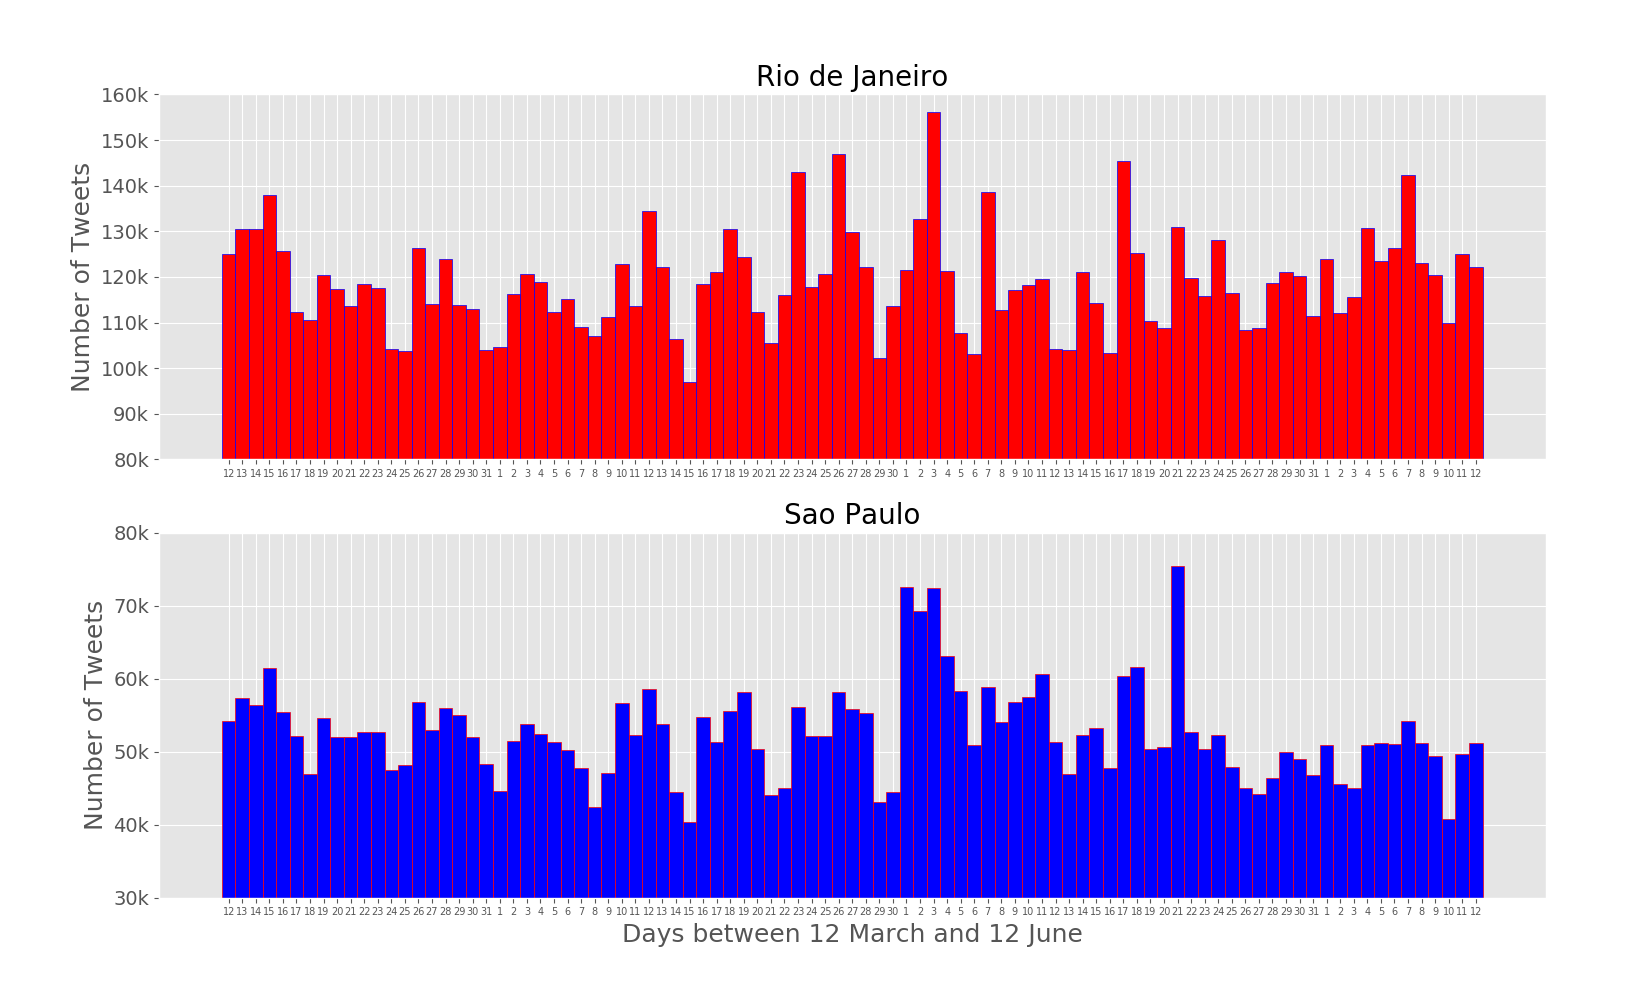
\includegraphics[width=\linewidth]{figures/rio_sp_whole_months.png}
		\caption{}
		\label{subfig:portuguese_cities_whole_months} 
	\end{subfigure}
	
	\begin{subfigure}[htbp]{0.8\textwidth}
		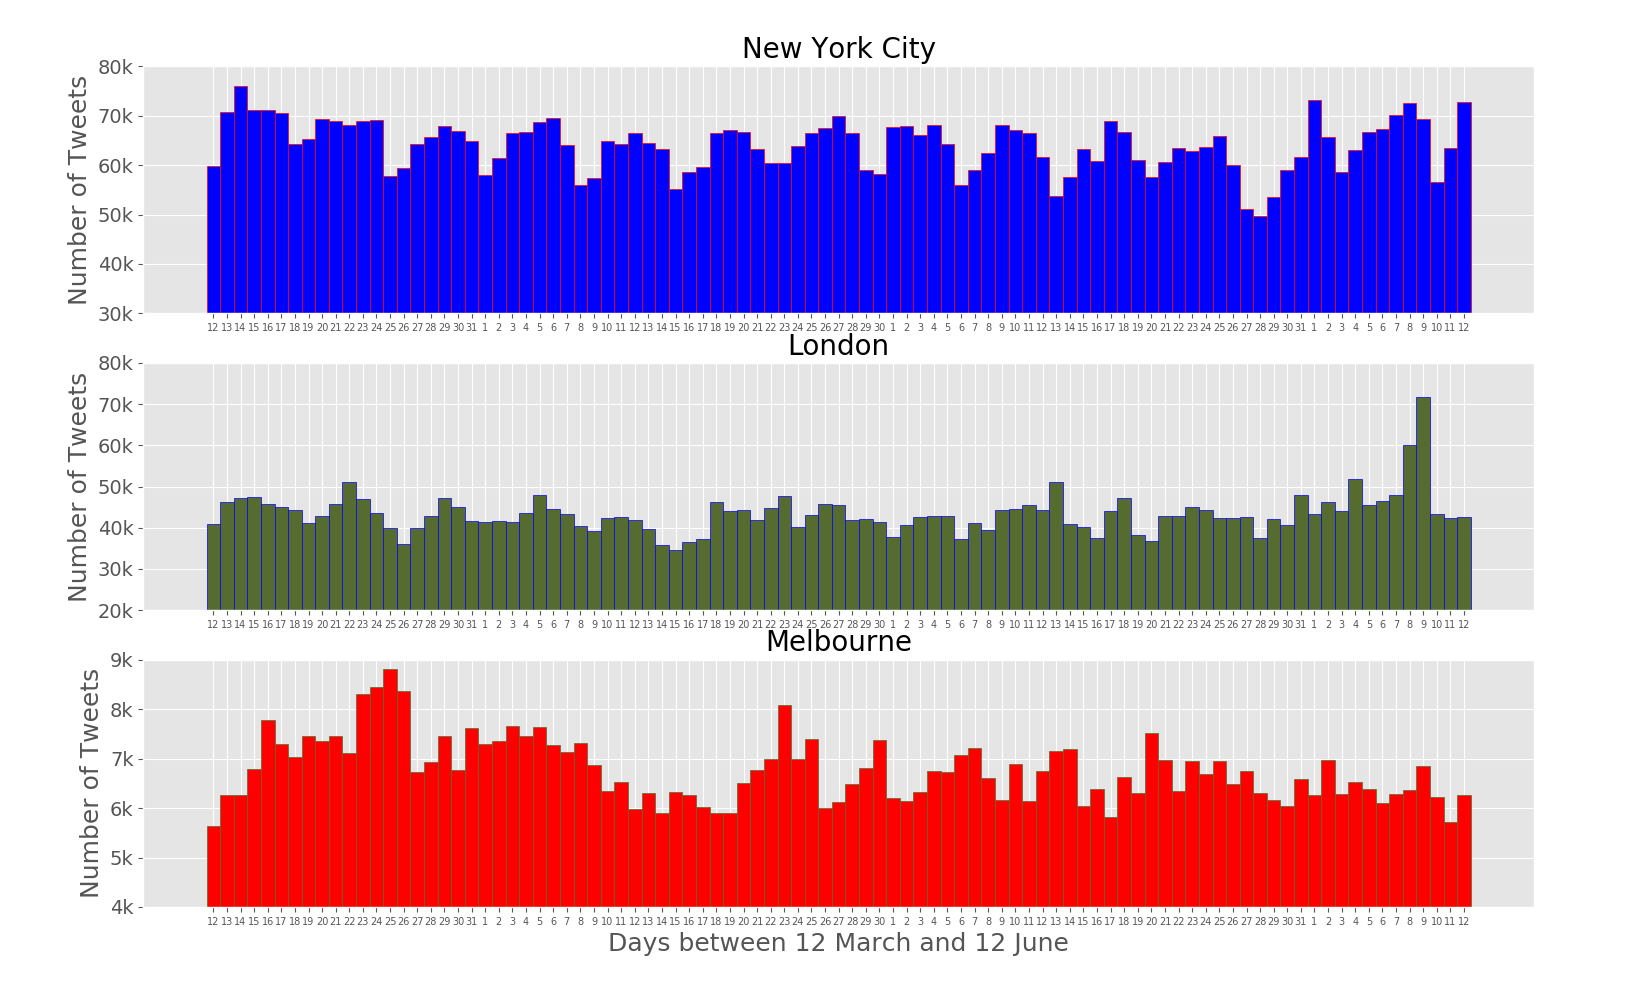
\includegraphics[width=\linewidth]{figures/nyc_london_melbourne_whole_months.png}
		\caption{}
		\label{subfig:english_cities_whole_months}
	\end{subfigure}
	
	\caption[Two numerical solutions]{(a) Rio de Janeiro and São Paulo - Portuguese Cities (b) New York City, London and Melbourne - English Cities}
	\label{fig:daily_distribution}
\end{figure}

During and after remarkable events, citizens are impelled to share their feelings, opinions or even report their safety and well-being conditions (e.g. in cases of terrorist attack) through mobile applications. This share of information increases the activity of social media platforms, which can be potentially used for the identification of uncommon events. Figure~\ref{fig:daily_distribution} illustrates the daily distribution of all cities for the period of collection, three whole months, between 12 March and 12 June, 2017. The Brazilian cities present high level of variation between consecutive days (with the volume varying in a tens of thousands of tweets) and so the task of identifying remarkable events turns out to be much harder. On the other hand, the English speaking cities in our study are very similar, with exception of Melbourne whose activity is very low comparatively to the other cities (New York City and London). In the particular case of London, we can identify an abrupt increase of volume during days 8 and 9 of June. With the support of external sources such as news websites, we learnt about the United Kingdom General Elections 2017~\footnote{\url{https://www.theguardian.com/politics/general-election-2017} (Accessed on 17/06/2017)} occurred on that period which suggests that an increase of the Twitter activity might be associated with that event. 

\begin{figure}[htbp]
    \centering
    \begin{subfigure}[htbp]{0.45\textwidth}
        \centering
        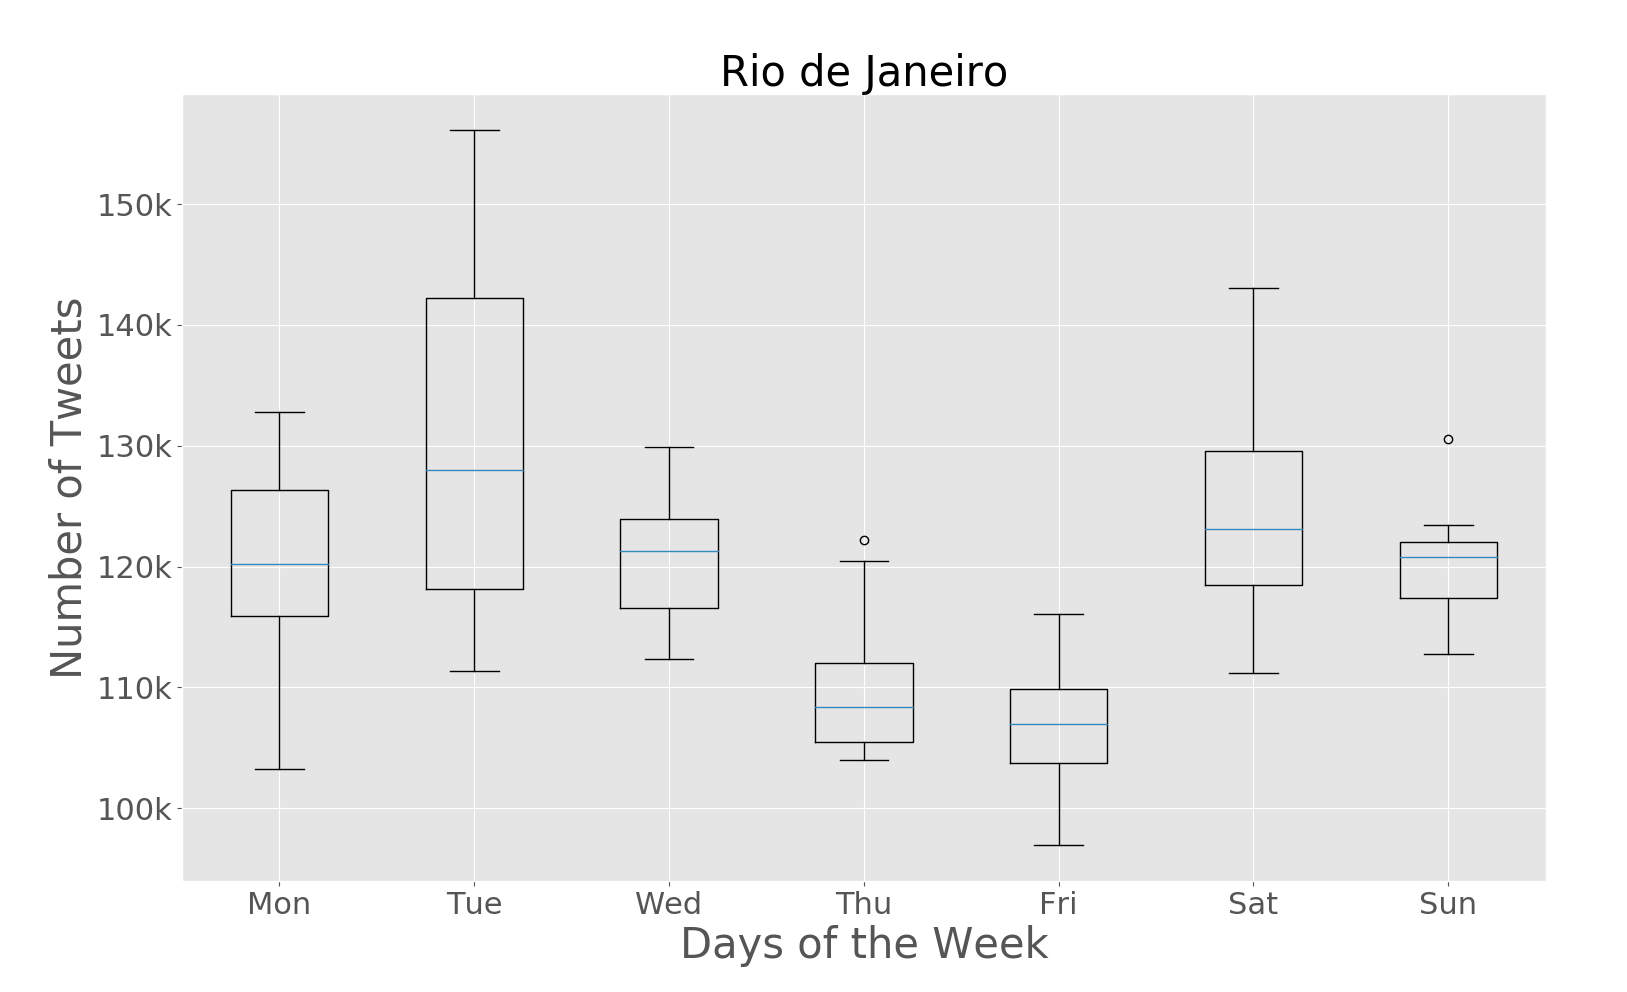
\includegraphics[width=1\linewidth]{figures/rio_box_plt_day_of_week.png}
        \caption{}
        \label{subfig:riodejaneiro_box_plot_day_of_week}
    \end{subfigure}%
    \quad
    \begin{subfigure}[htbp]{0.45\textwidth}
        \centering
        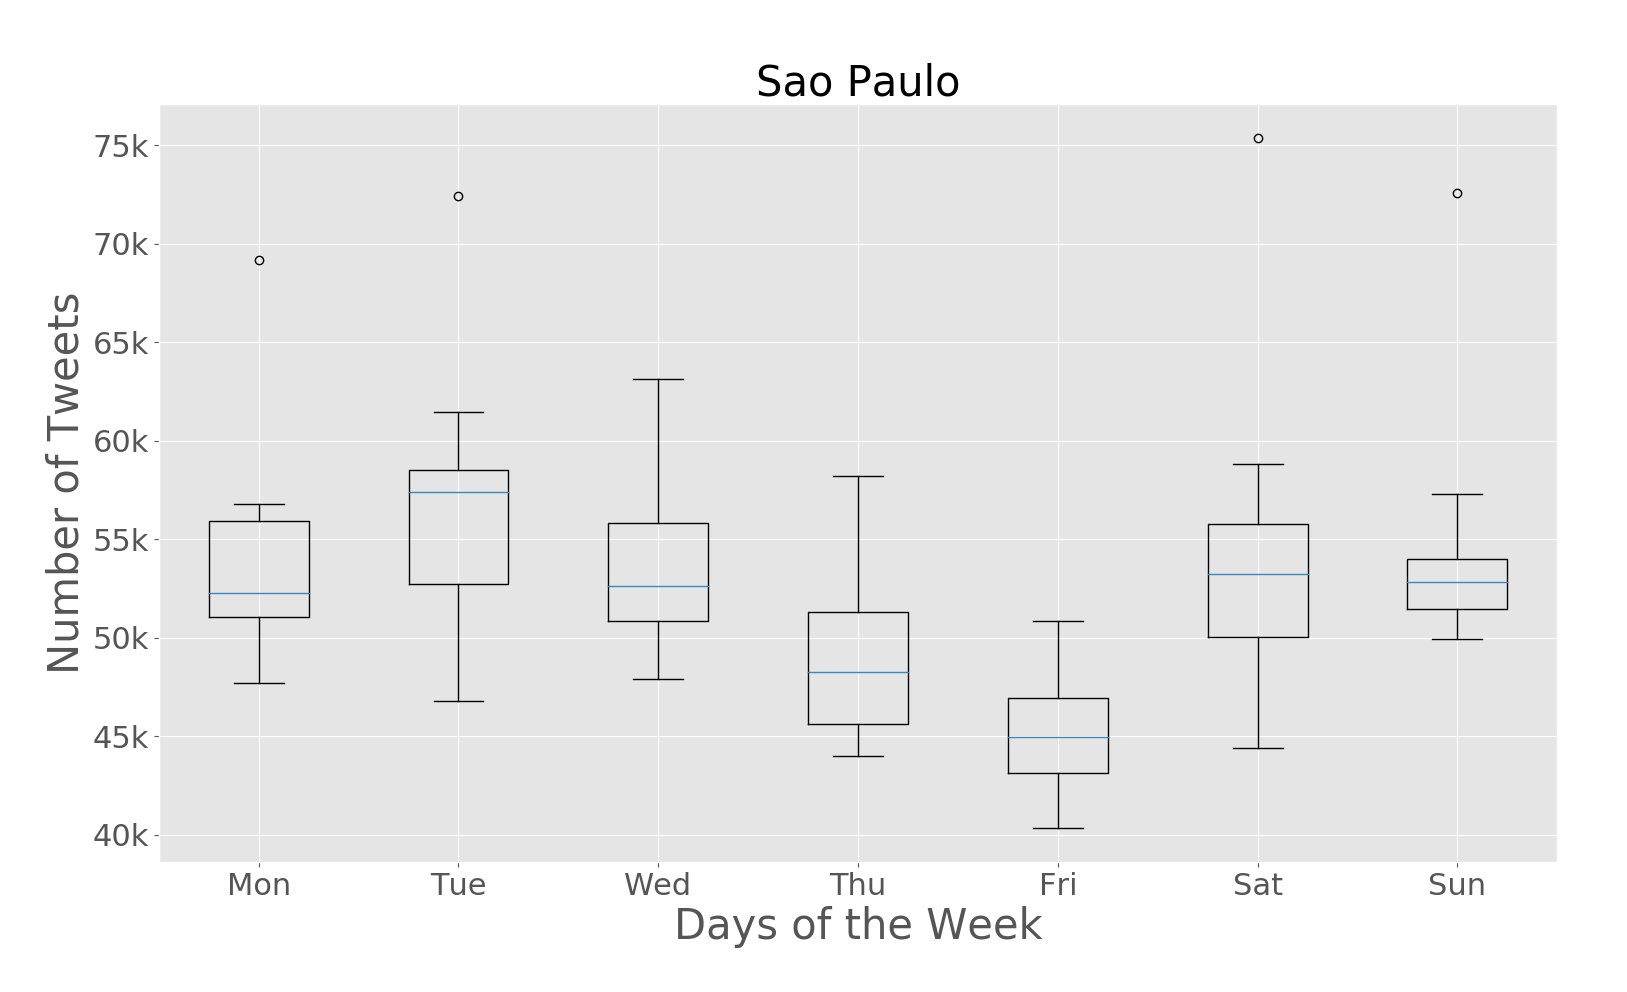
\includegraphics[width=1\linewidth]{figures/sp_box_plt_day_of_week.png}
        \caption{}
        \label{subfig:saopaulo_box_plot_day_of_week}
    \end{subfigure}

    \medskip

    \begin{subfigure}[htbp]{0.45\textwidth}
        \centering
        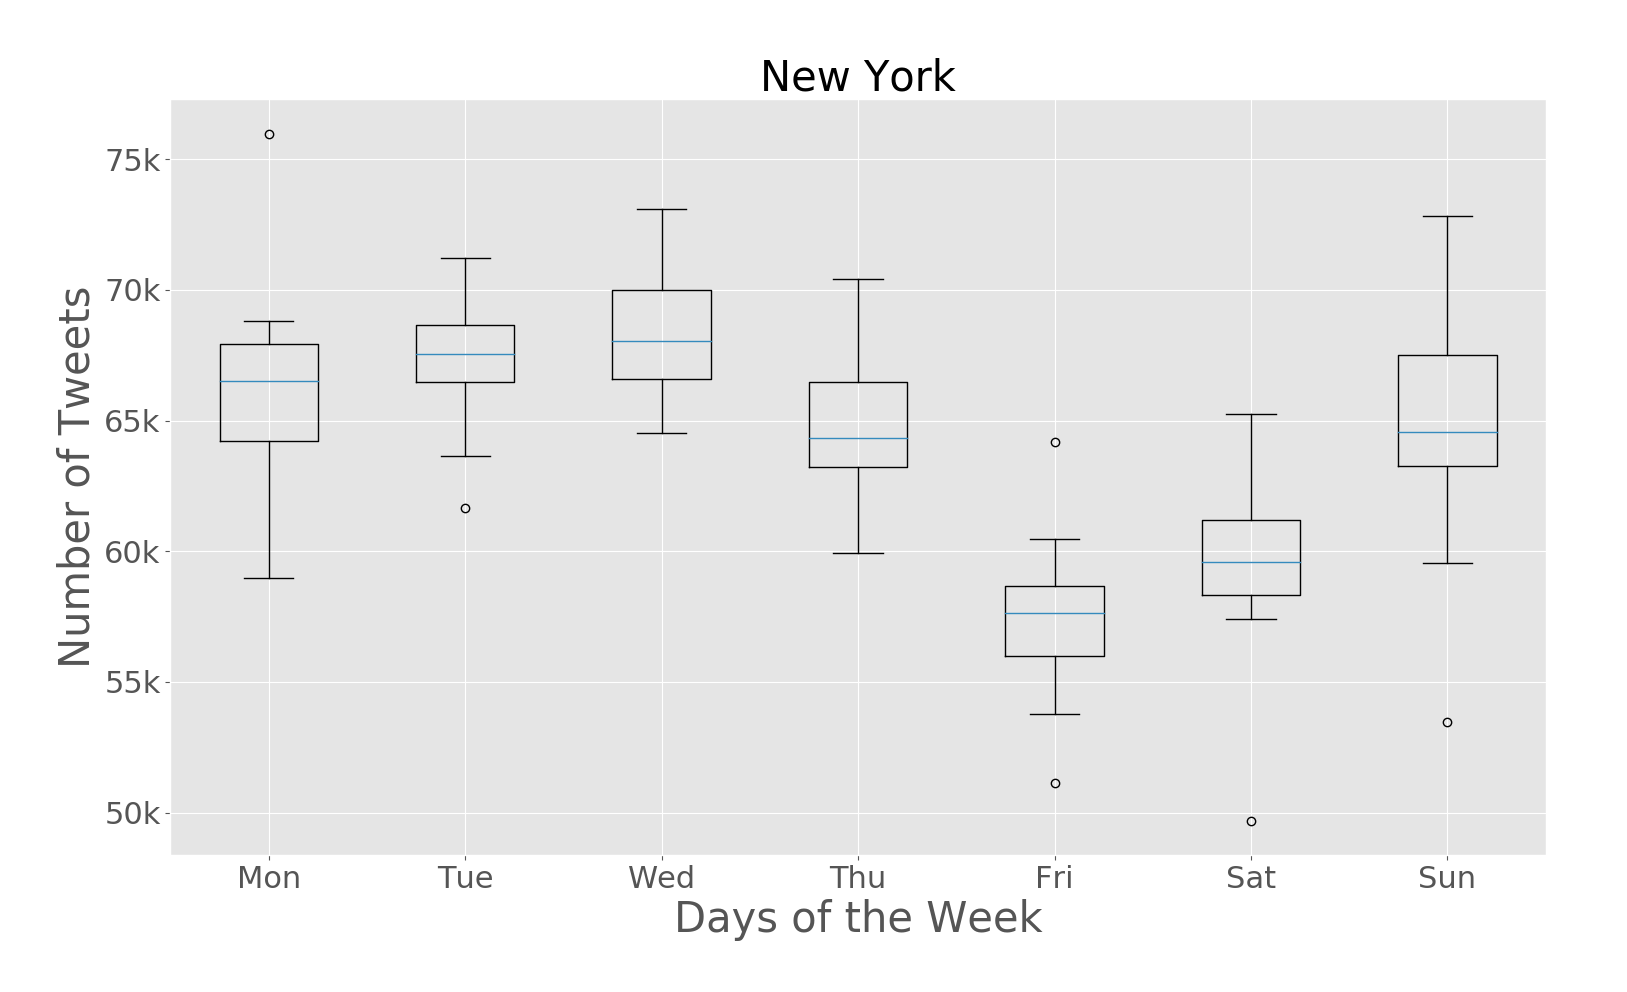
\includegraphics[width=1\linewidth]{figures/nyc_box_plt_day_of_week.png}
        \caption{}
        \label{subfig:newyork_box_plot_day_of_week}
    \end{subfigure}
    \quad
    \begin{subfigure}[htbp]{0.45\textwidth}
        \centering
        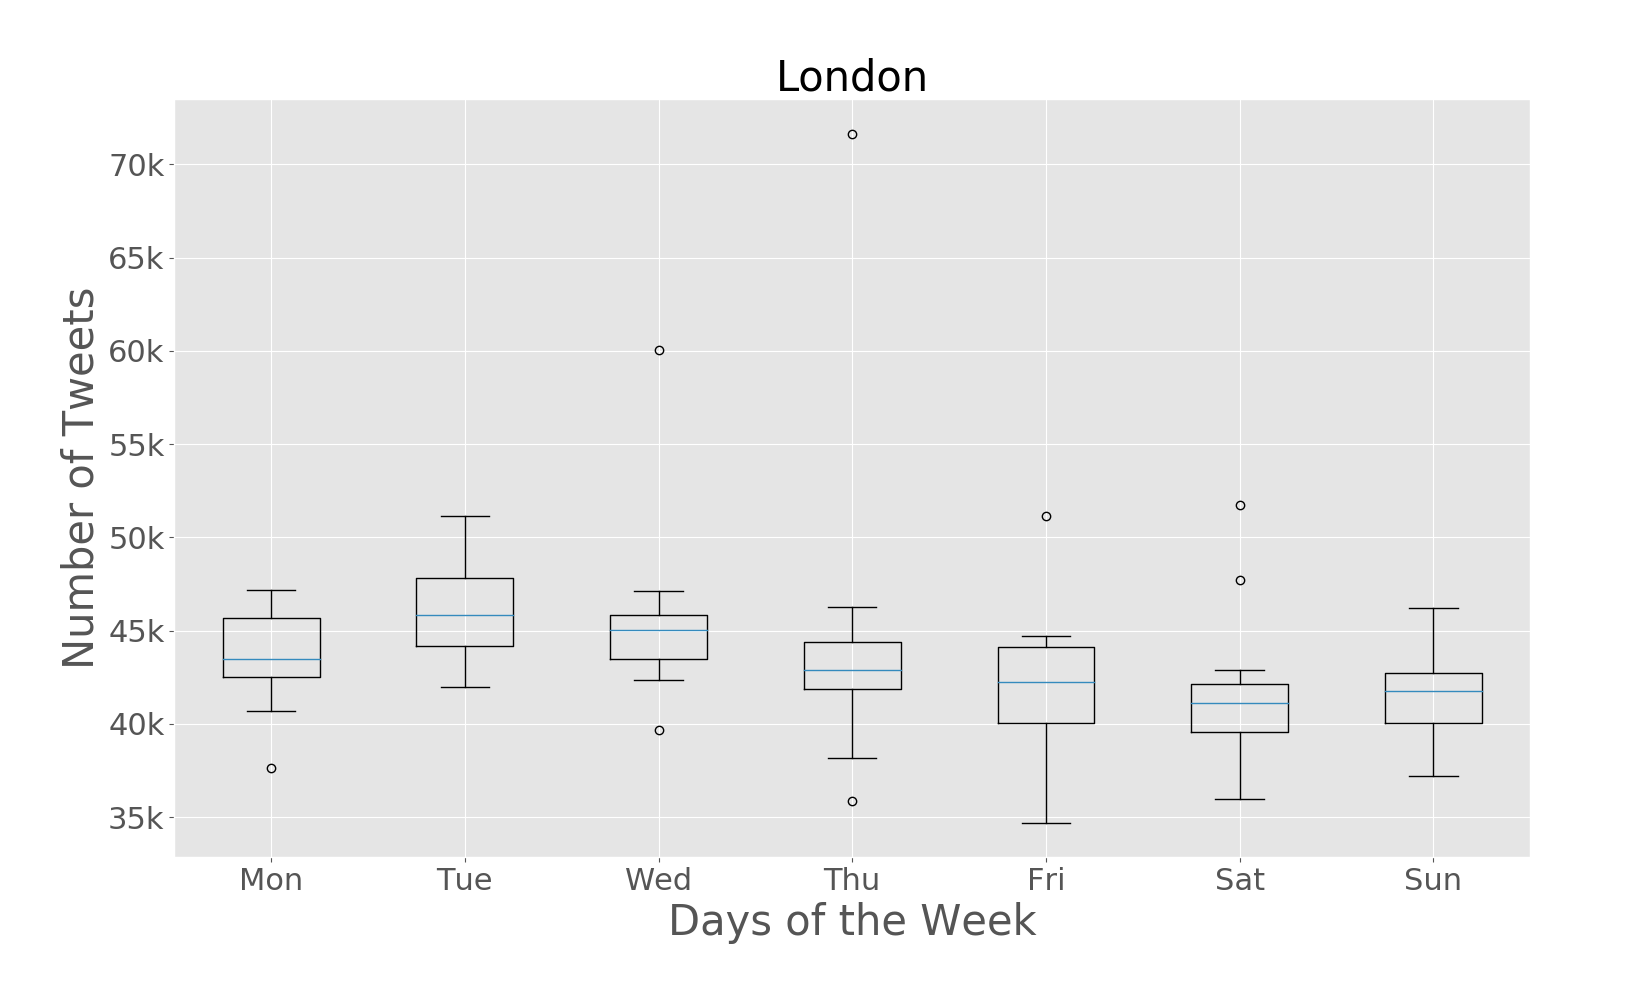
\includegraphics[width=1\linewidth]{figures/london_box_plt_day_of_week.png}
        \caption{}
        \label{subfig:london_box_plot_day_of_week}
    \end{subfigure}

	\medskip
    
     \begin{subfigure}[htbp]{0.45\textwidth}
        \centering
        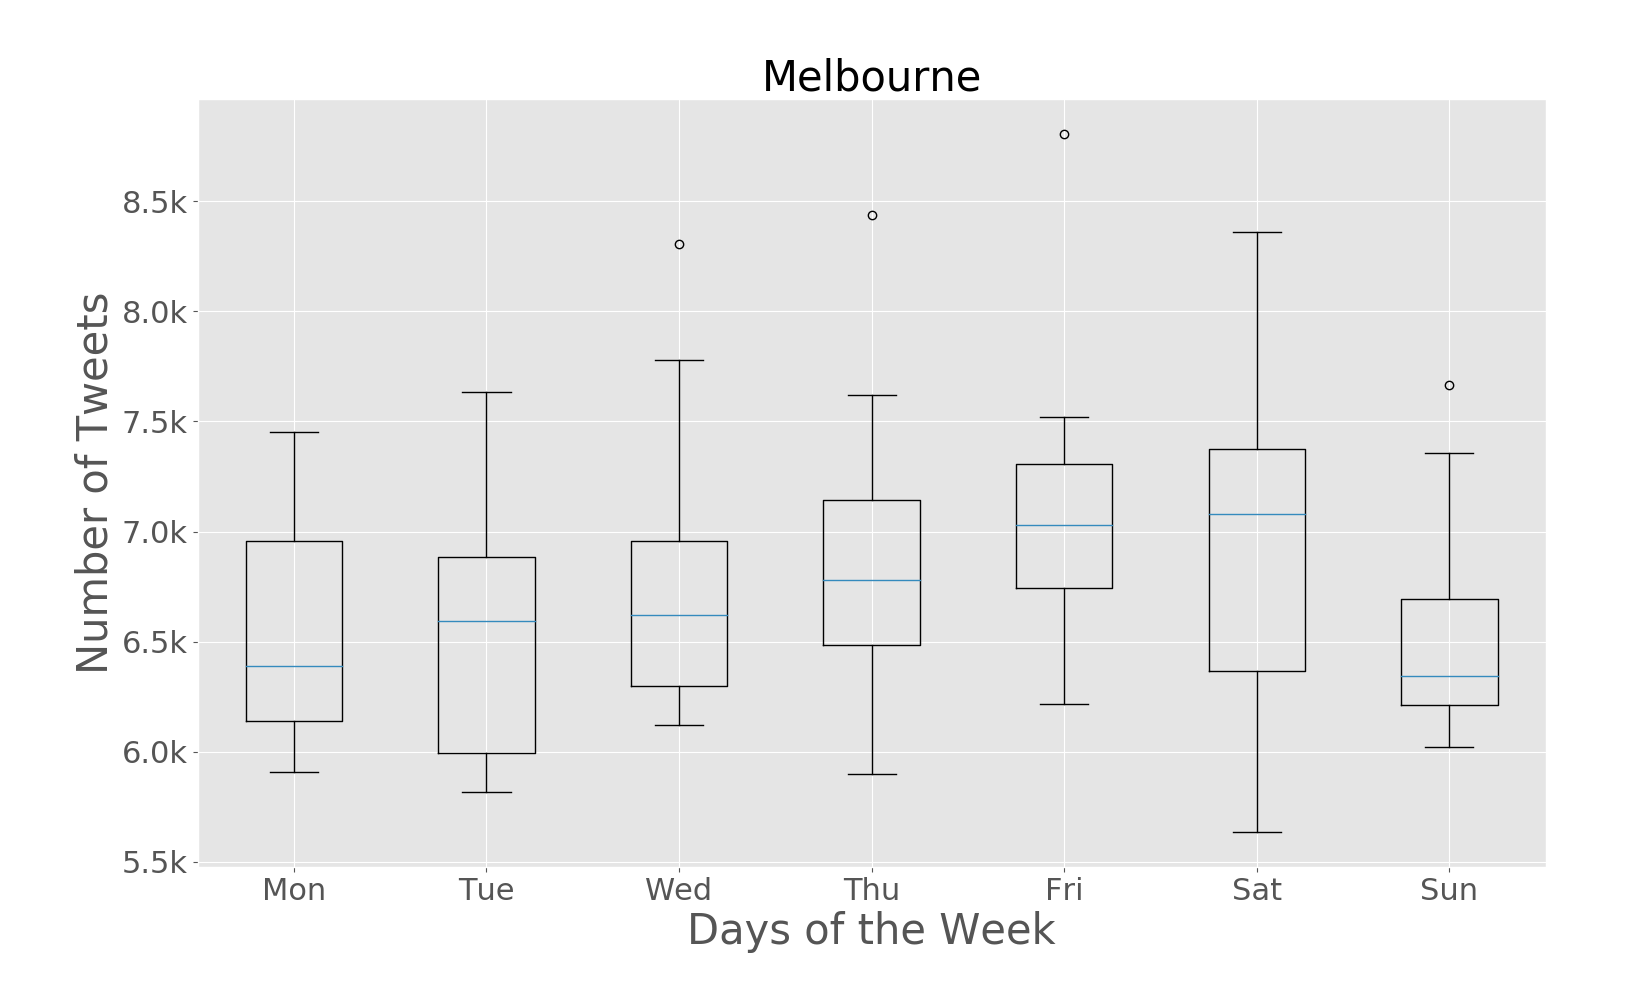
\includegraphics[width=1\linewidth]{figures/melbourne_box_plt_day_of_week.png}
        \caption{}
        \label{subfig:melbourne_box_plot_day_of_week}
    \end{subfigure}
    
\caption[Five numerical solutions]{Days-of-the-week box-plots for the volume of tweets (a) Rio de Janeiro (b) São Paulo (c) New York City (d) London (e) Melbourne}
\label{fig:box_plots_day_of_week}
\end{figure}

In order to understand the most active days and hours in Twitter, for all cities under this study, we aggregate the datasets by these attributes and represented the final results in a box plot representation. This type of data visualization allows, in a standardized way, the displaying of distributions of data based on the six different values: (1) minimum and (2) maximum values for each day/hour regarding the activity on Twitter; (3) median value for the each day/hour, (4) first and (5) third quartiles as well as (6) the interquartile range (IQR). Figures~\ref{fig:box_plots_day_of_week} and~\ref{fig:box_plots_hour_of_day} illustrated this type of data visualization for the whole three months of data collected. Taking into analysis the city of Rio de Janeiro, it was possible to observe and enhance Tuesdays as the day of the week where there is more activity on Twitter. Moreover, Fridays revealed to be the day less active, not only for the city of Rio de Janeiro, but for all remaining cities with exception of Melbourne. Particularly, the activity on Twitter in Melbourne is centered in the weekend days while the other cities the highest levels of activity is spread between week and weekend days. The interquartile range in the plots can tell us the amount of days whose activity was above and behold the median value, and through that we identify Rio de Janeiro and Melbourne as the cities where this phenomenon happen more times. São Paulo, New York City and London present an almost regular IQR which means that the days of weeks are similarly regarding the activity on Twitter.

\begin{figure}[htbp]
	\centering
	\begin{subfigure}[htbp]{0.45\textwidth}
		\centering
		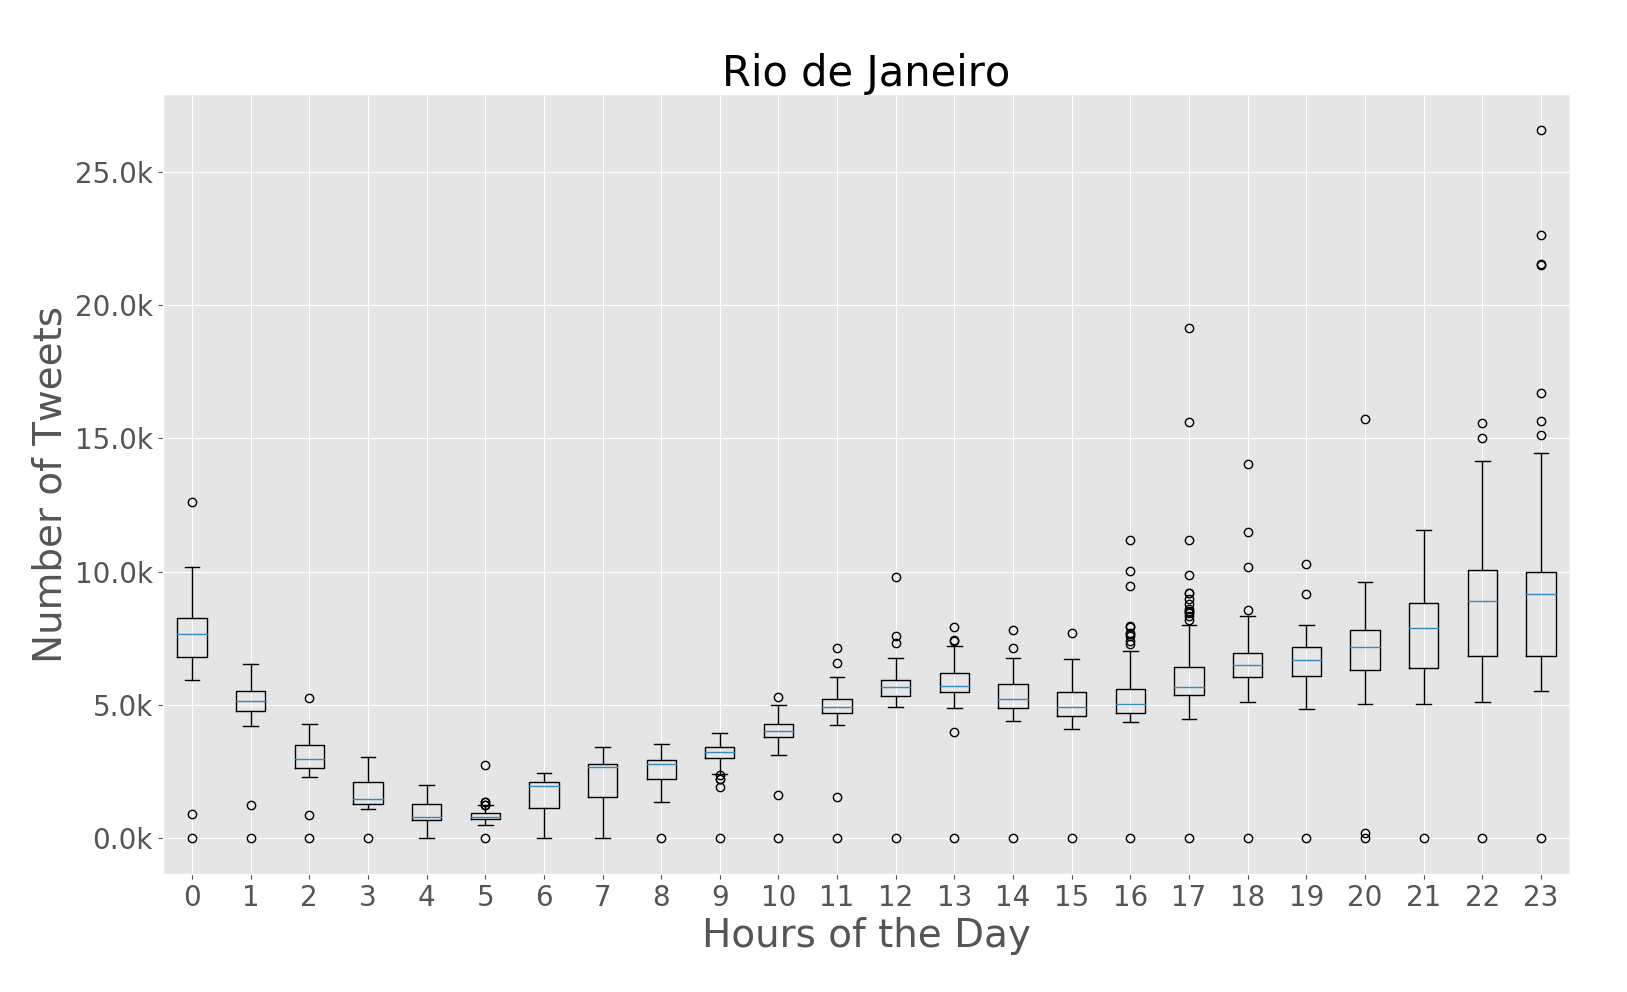
\includegraphics[width=1\linewidth]{figures/rio_box_plt_hour_of_day.png}
		\caption{}
		\label{subfig:riodejaneiro_box_plot_hour_of_day}
	\end{subfigure}%
	\quad
	\begin{subfigure}[htbp]{0.45\textwidth}
		\centering
		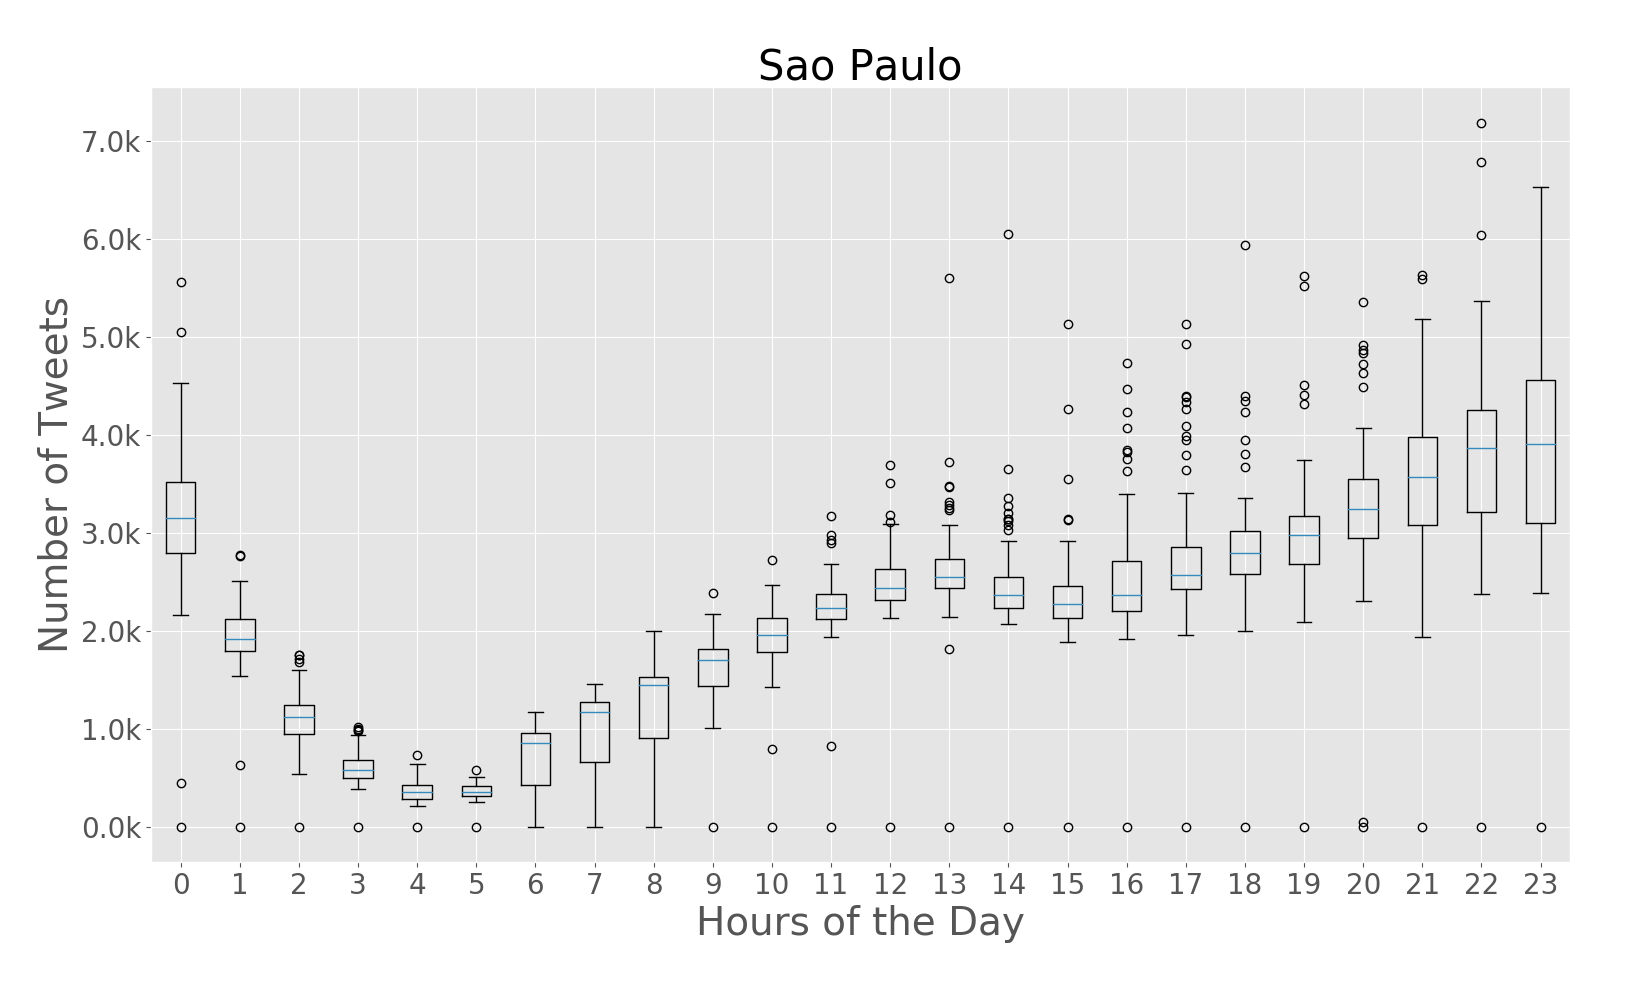
\includegraphics[width=1\linewidth]{figures/sp_box_plt_hour_of_day.png}
		\caption{}
		\label{subfig:saopaulo_box_plot_hour_of_day}
	\end{subfigure}
	
	\medskip
	
	\begin{subfigure}[htbp]{0.45\textwidth}
		\centering
		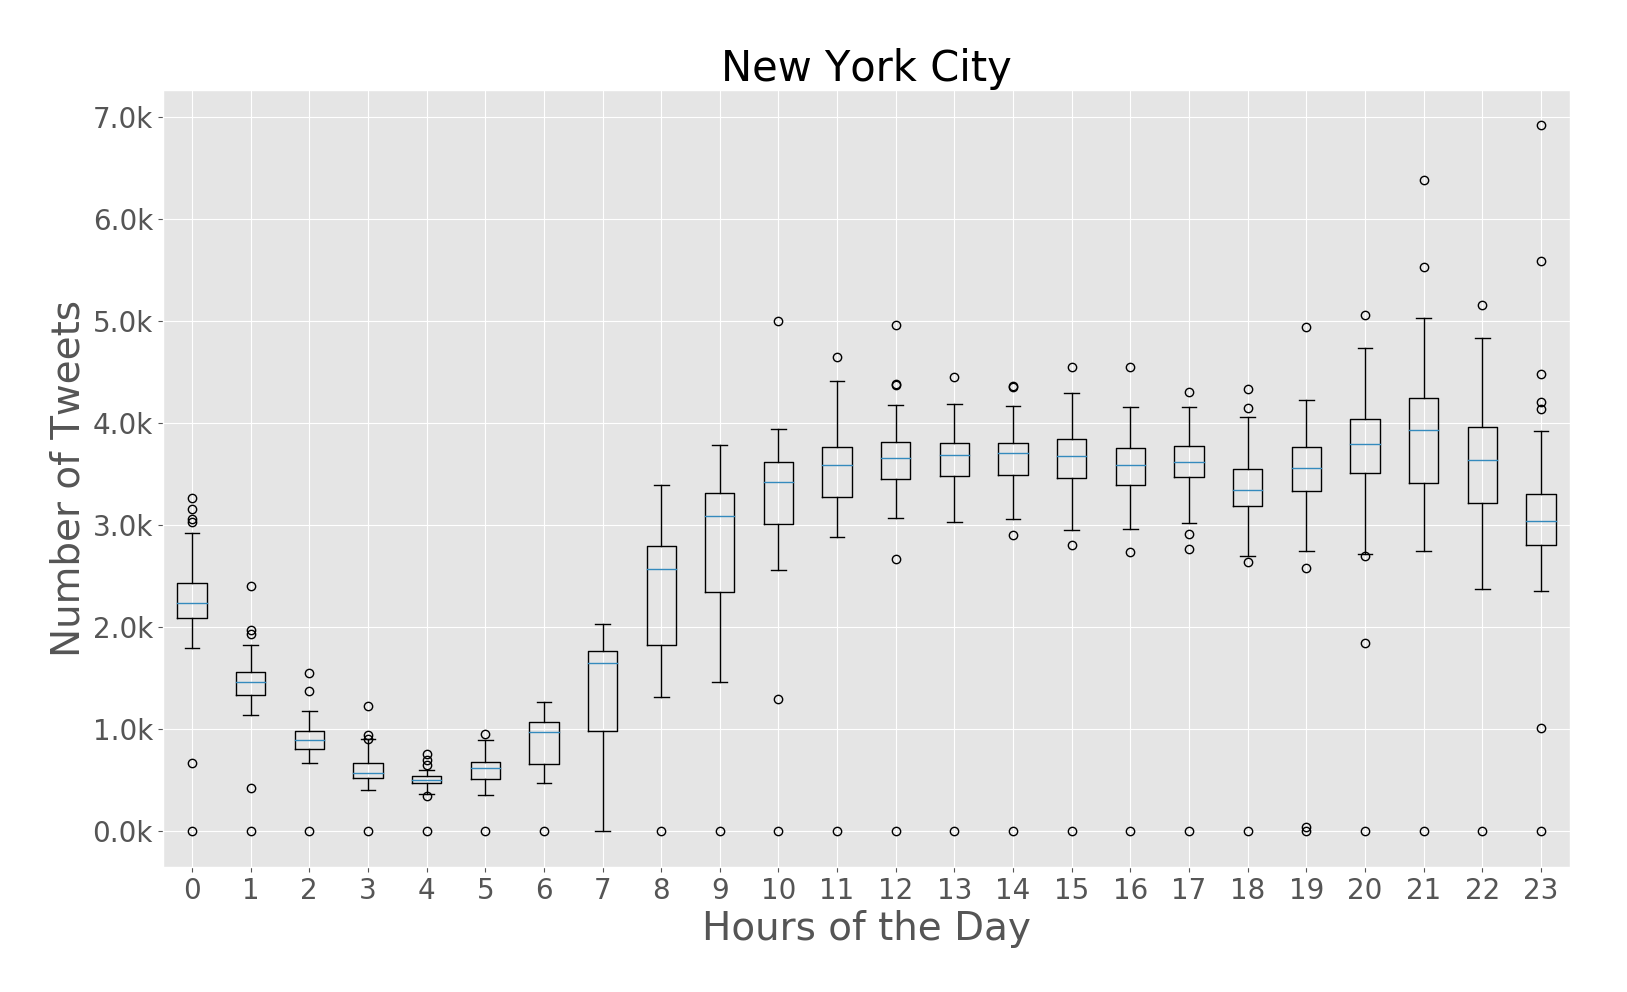
\includegraphics[width=1\linewidth]{figures/nyc_box_plt_hour_of_day.png}
		\caption{}
		\label{subfig:newyork_box_plot_hour_of_day}
	\end{subfigure}
	\quad
	\begin{subfigure}[htbp]{0.45\textwidth}
		\centering
		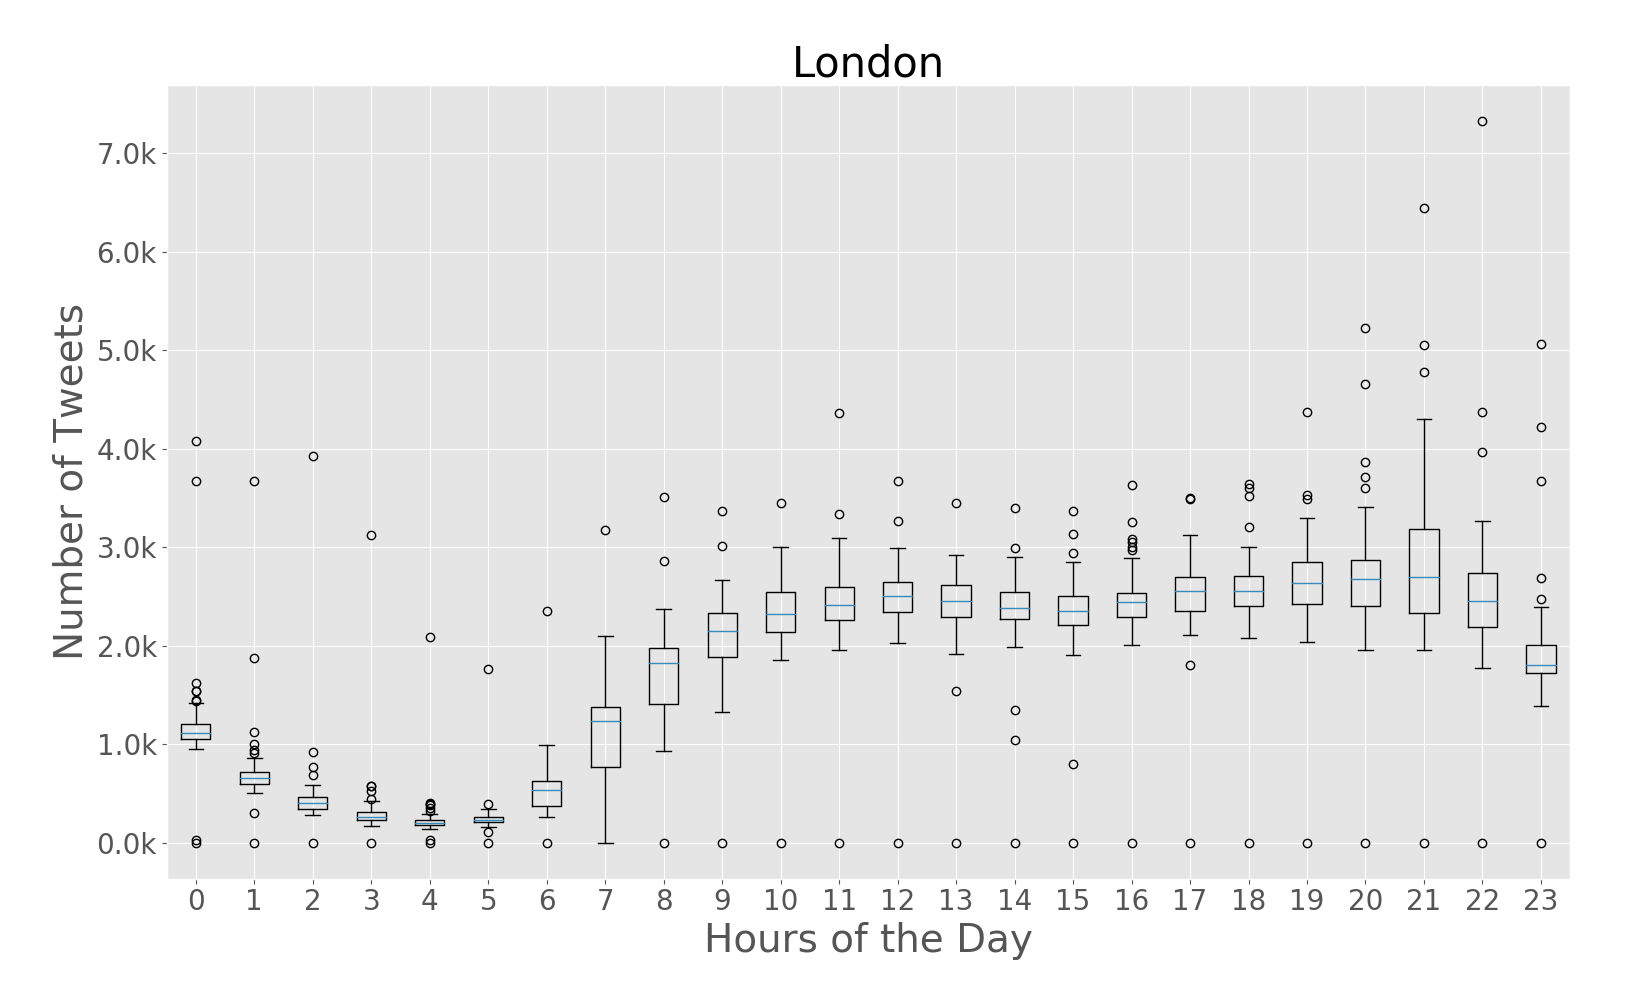
\includegraphics[width=1\linewidth]{figures/london_box_plt_hour_of_day.png}
		\caption{}
		\label{subfig:london_box_plot_hour_of_day}
	\end{subfigure}
	
	\medskip
	
	\begin{subfigure}[htbp]{0.45\textwidth}
		\centering
		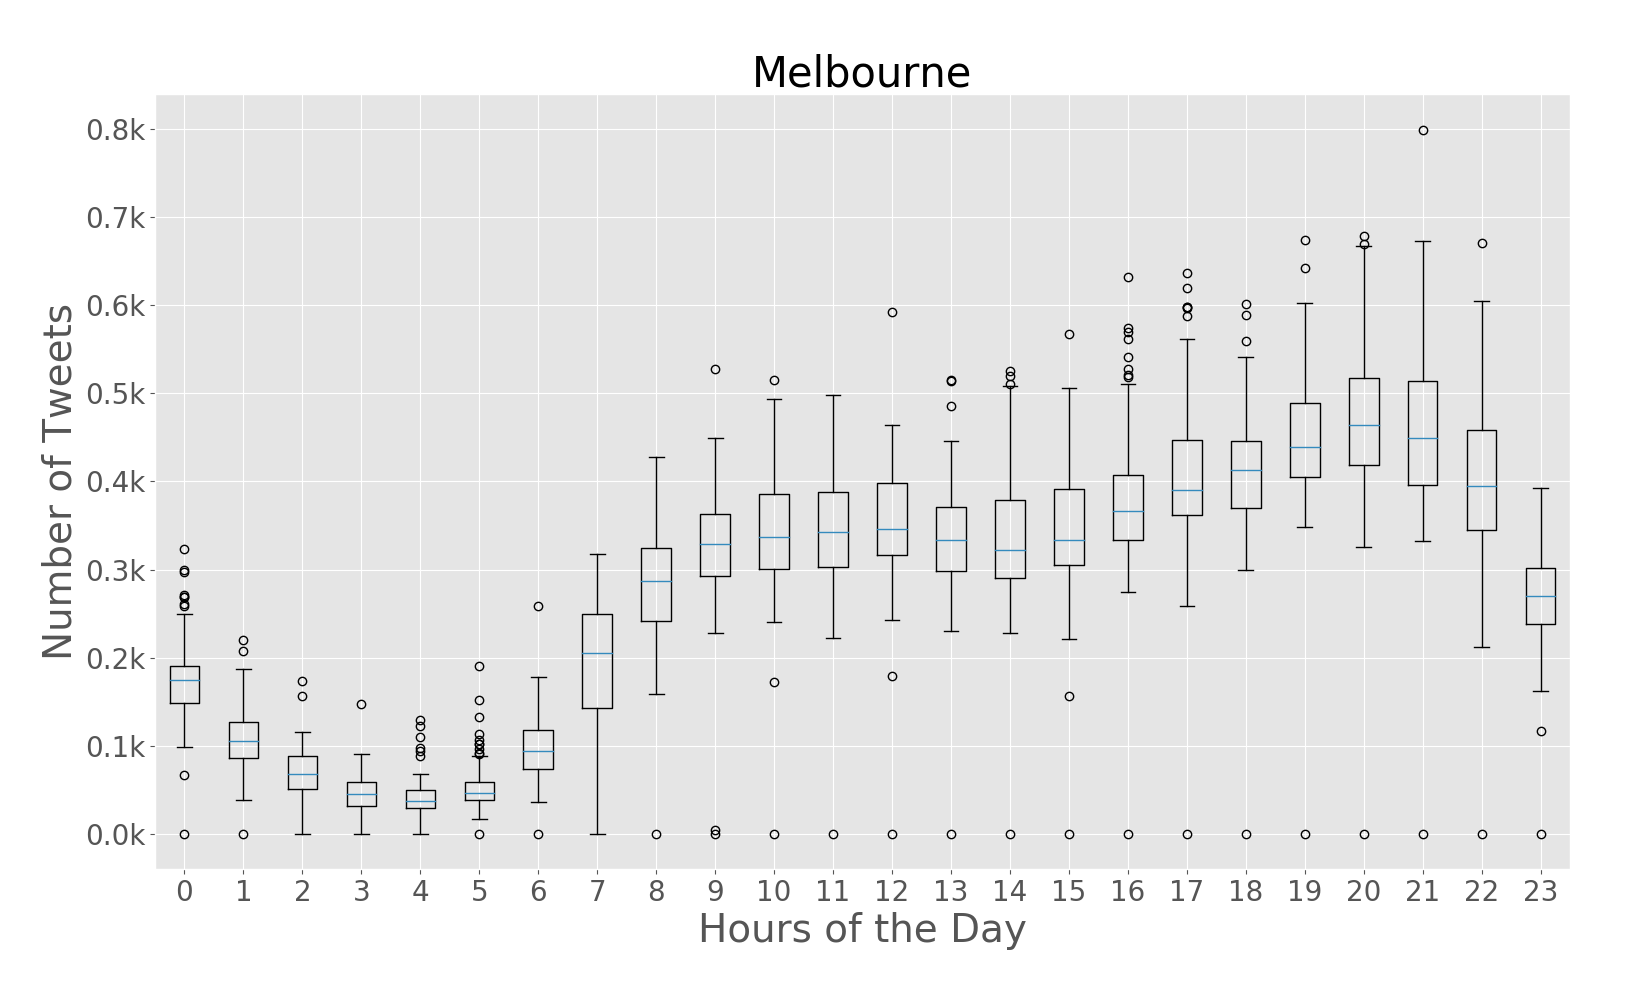
\includegraphics[width=1\linewidth]{figures/melbourne_box_plt_hour_of_day.png}
		\caption{}
		\label{subfig:melbourne_box_plot_hour_of_day}
	\end{subfigure}
	
	\caption[Five numerical solutions]{Hours-of-the-day box-plots for the volume of tweets (a) Rio de Janeiro (b) São Paulo (c) New York City (d) London (e) Melbourne}
	\label{fig:box_plots_hour_of_day}
\end{figure}

Looking at the hour-of-the-day box-plot (\ref{fig:box_plots_hour_of_day}), it is possible to verify an decrease in terms of activity on Twitter during the night period to all cities. More specifically, there were cases in which the volume of tweets was inexistent and based on this fact, two possible reason are suggested: (1) the absence of tweets during this period is explained through the zero activity of users in the city, regarding geo-located tweets; (2) the service on Twitter was in maintenance and due to that, any tweet was retrieved by the API. Although the observable increase of activity during day-time, the peak of it is similiar to all cities and it is established between the 19 and 23 hours.

\subsection{Content Composition}

Tweets although its classification as text messages, also contain other kind of \textit{metadata} which exploration of it can sometimes be transformed in added-value information. The \textit{metadata} present in a tweet is represented by the \textit{hashtags}, \textit{user mentions}, \textit{URLs} and \textit{media} attached to it. Other point to explore is the number of distinct users that contributed to the datasets composition. Users which number of posts are unnatural may sometimes be \textit{bots}. If there is a time pattern associated to the post of tweets by a user, for example, the user posts a tweet in a period of 5 minutes over the whole day, then this user is a potential \textit{bot}. The existence of \textit{bots} is not considered in this dissertation because the information provide by such automatic system can also be valuable. In this subsection, we demonstrated the distribution of users over the number of posts made by themselves, as well as the counts of the different type of \textit{metadata }contained in the data. 

Social media platforms present similar characteristics between themselves. One of the most studied ones is the behviour of the its users activity in its services (social media services). The visualization of users activity usually is similar to the power-law distribution long tail~\cite{muchnik2013origins}. Here, we tried to reproduce such visualization in order to establish this kind of correlation as so to prove this behaviour over social media services. The results are present in Figure~\ref{fig:loglog-plots-users}. Each city proved to have a high number of users with few posts and that is observable in the long-tail showed in the cities corresponding sub-figures (~\ref{subfig:riodejaneiro_loglog_users},~\ref{subfig:saopaulo_loglog_users},~\ref{subfig:newyork_loglog_users},~\ref{subfig:london_loglog_users},~\ref{subfig:melbourne_loglog_users}).

The counts and percentages of users that have posted a certain number of tweets was calculated in order to assure the trustiness of the aforementioned distribution. Rio de Janeiro although the highest number of tweets in the datasets only was composed by 135,449 distinct users followed by São Paulo with a lower number 110,352 individuals. The English speaking cities revealed to be very different comparatively to the Portuguese speaking cities in this factor. New York City dataset was composed by 279,554 distinct users, London presented 266,128 users and Melbourne only was composed by 31,733 individuals. Looking at these numbers, we may conclude that Rio de Janeiro has a high percentage of users with more than a certain number of tweets and following this assumption, the log-log distribution made to correlate the behaviour of a power-law distribution must be different from the other cities, at least the English speaking ones.

For example, the percentage of users that posted 20 tweets in a period of three months was almost 63\% for the city of Rio de Janeiro, São Paulo registered 75\%, New York City presented 84\%, London showed 87\% while Melbourne had 87\% of his users with that number of tweets shared. Only taking this example in consideration we proved the assumption mentioned before. The distributions also presented differences if the x-axis is considered. The scale at such axis is one magnitude higher for the English speaking cities, and this means that the number of users with lower number of tweets posted in a three months period is much higher than the users with the same number for the city of Rio de Janeiro.

\begin{figure}[h]
	\centering
	\begin{subfigure}[t]{0.45\textwidth}
		\centering
		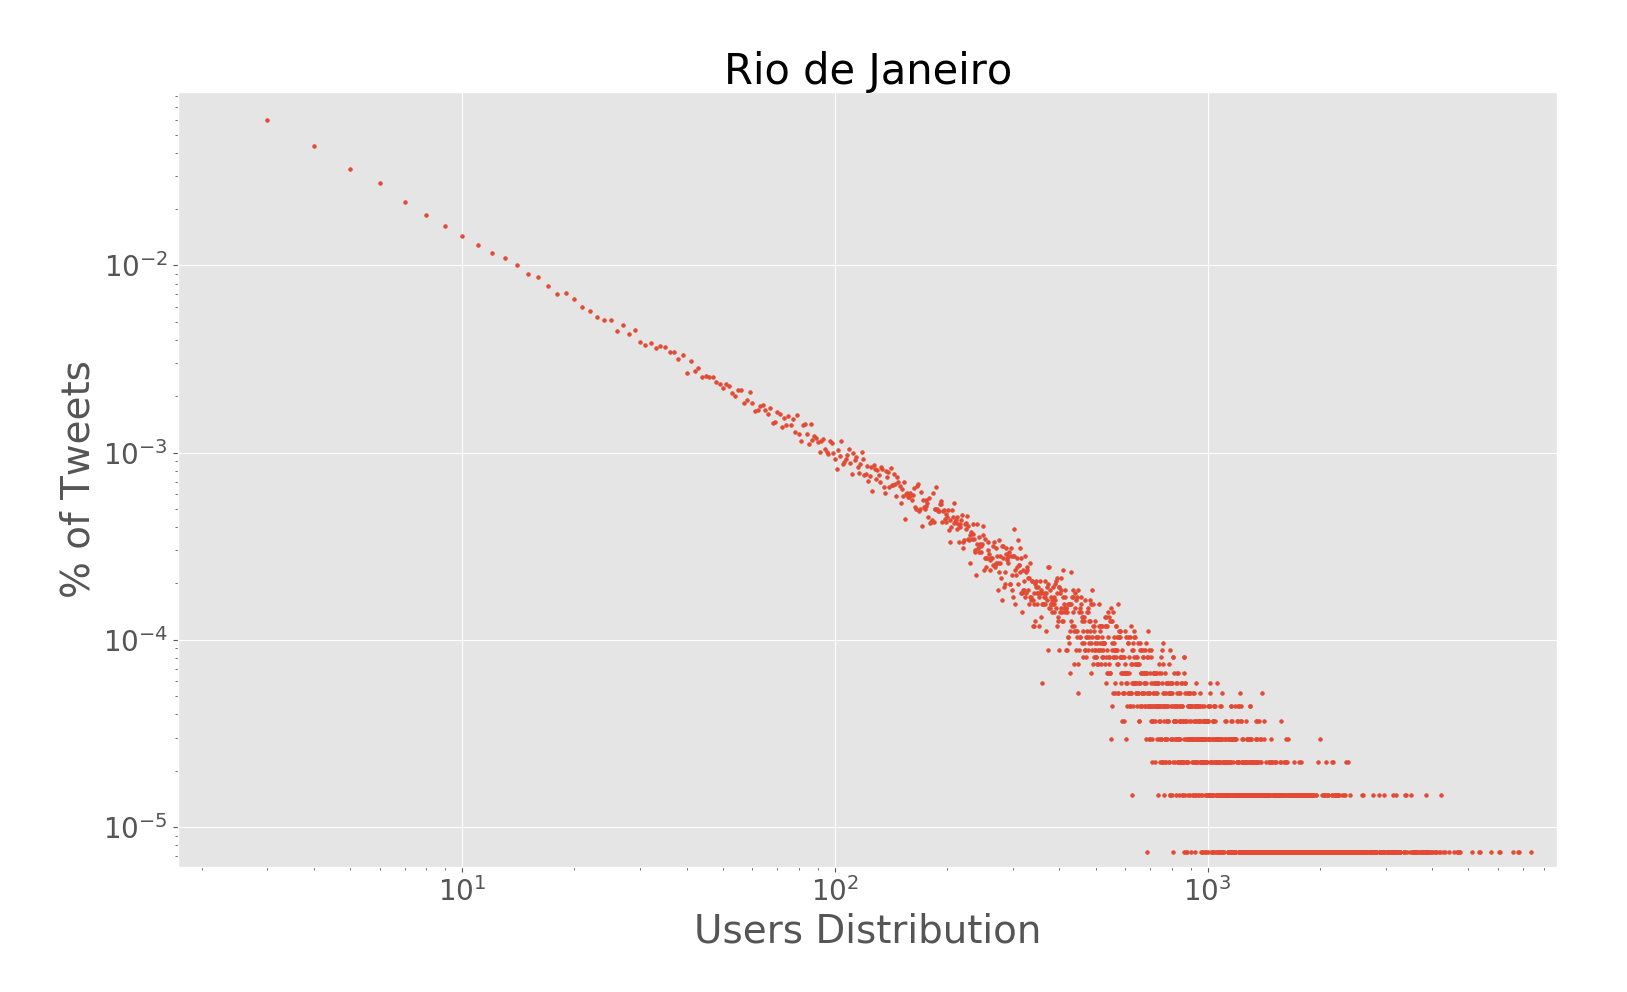
\includegraphics[width=1\linewidth]{figures/rio_loglog_users.png}
		\caption{}
		\label{subfig:riodejaneiro_loglog_users}
	\end{subfigure}%
	\quad
	\begin{subfigure}[t]{0.45\textwidth}
		\centering
		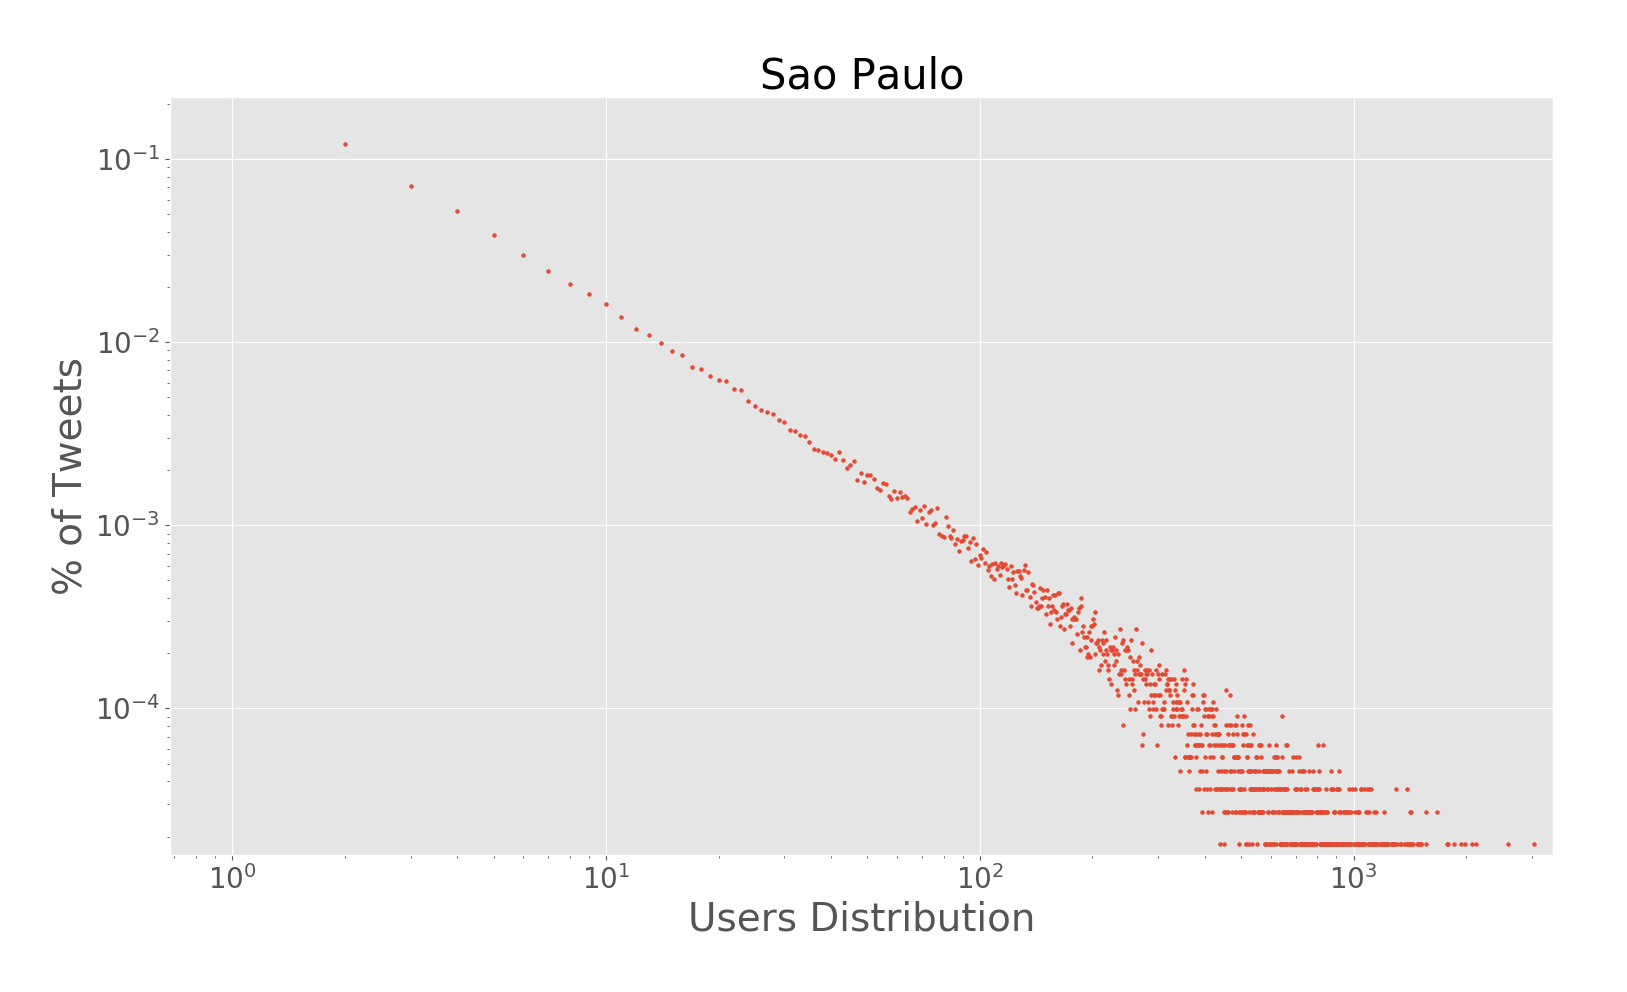
\includegraphics[width=1\linewidth]{figures/sp_loglog_users.png}
		\caption{}
		\label{subfig:saopaulo_loglog_users}
	\end{subfigure}
	
	\medskip
	
	\begin{subfigure}[t]{0.45\textwidth}
		\centering
		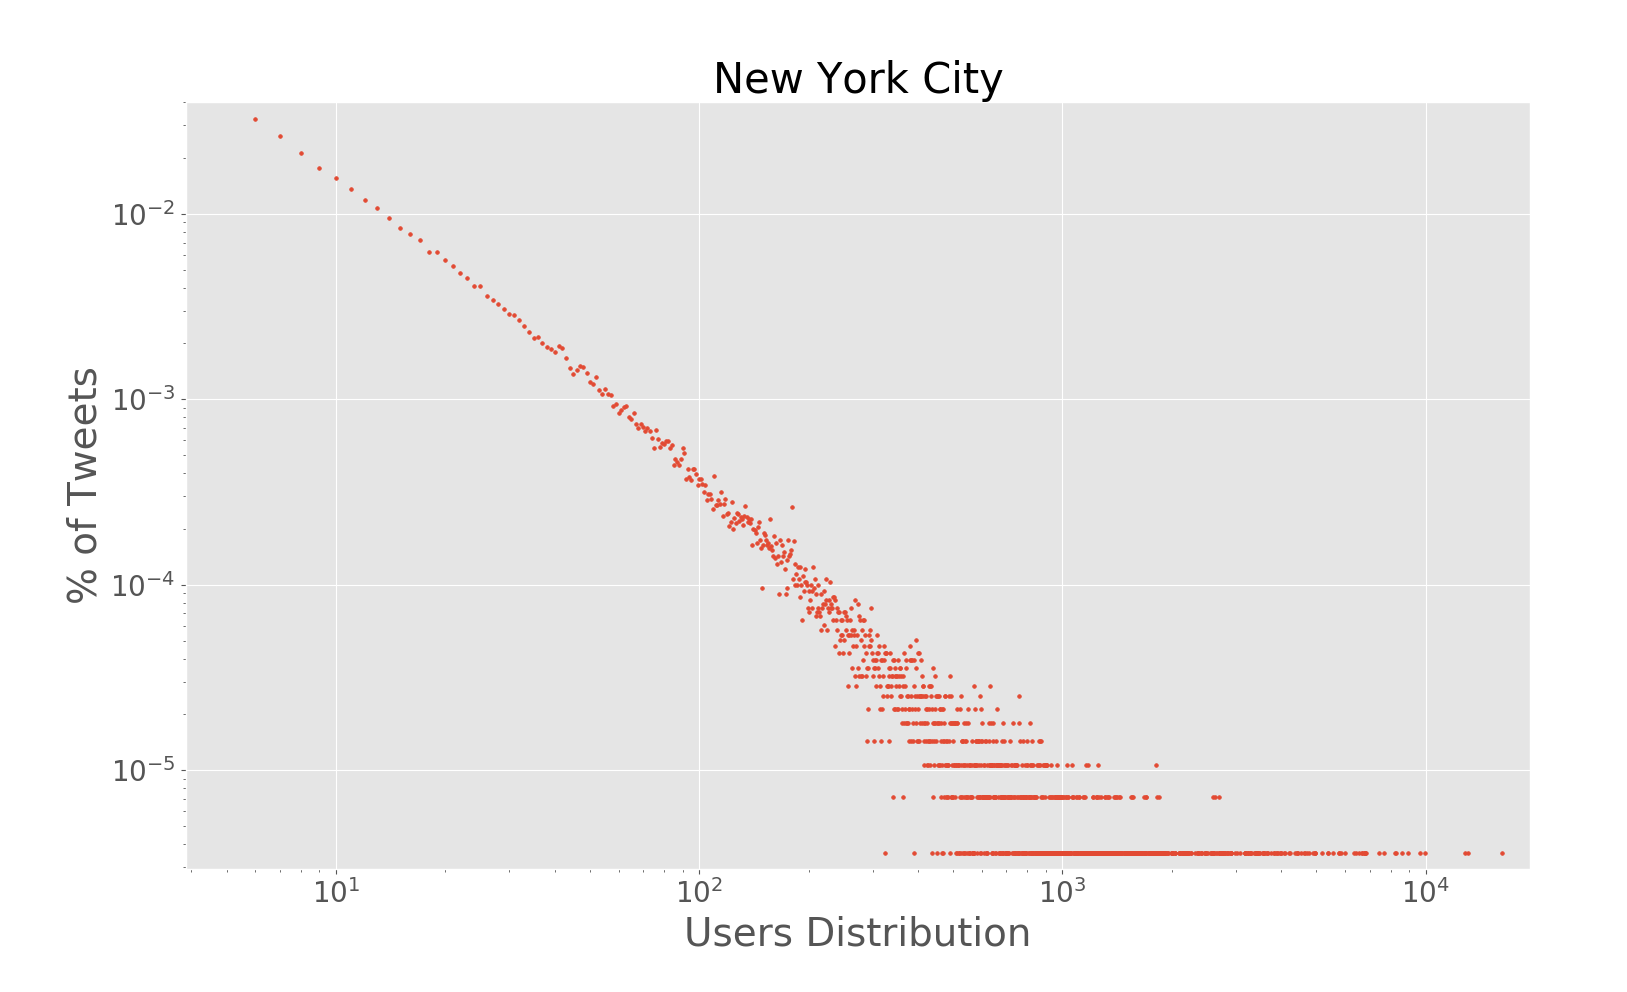
\includegraphics[width=1\linewidth]{figures/nyc_loglog_users.png}
		\caption{}
		\label{subfig:newyork_loglog_users}
	\end{subfigure}
	\quad
	\begin{subfigure}[t]{0.45\textwidth}
		\centering
		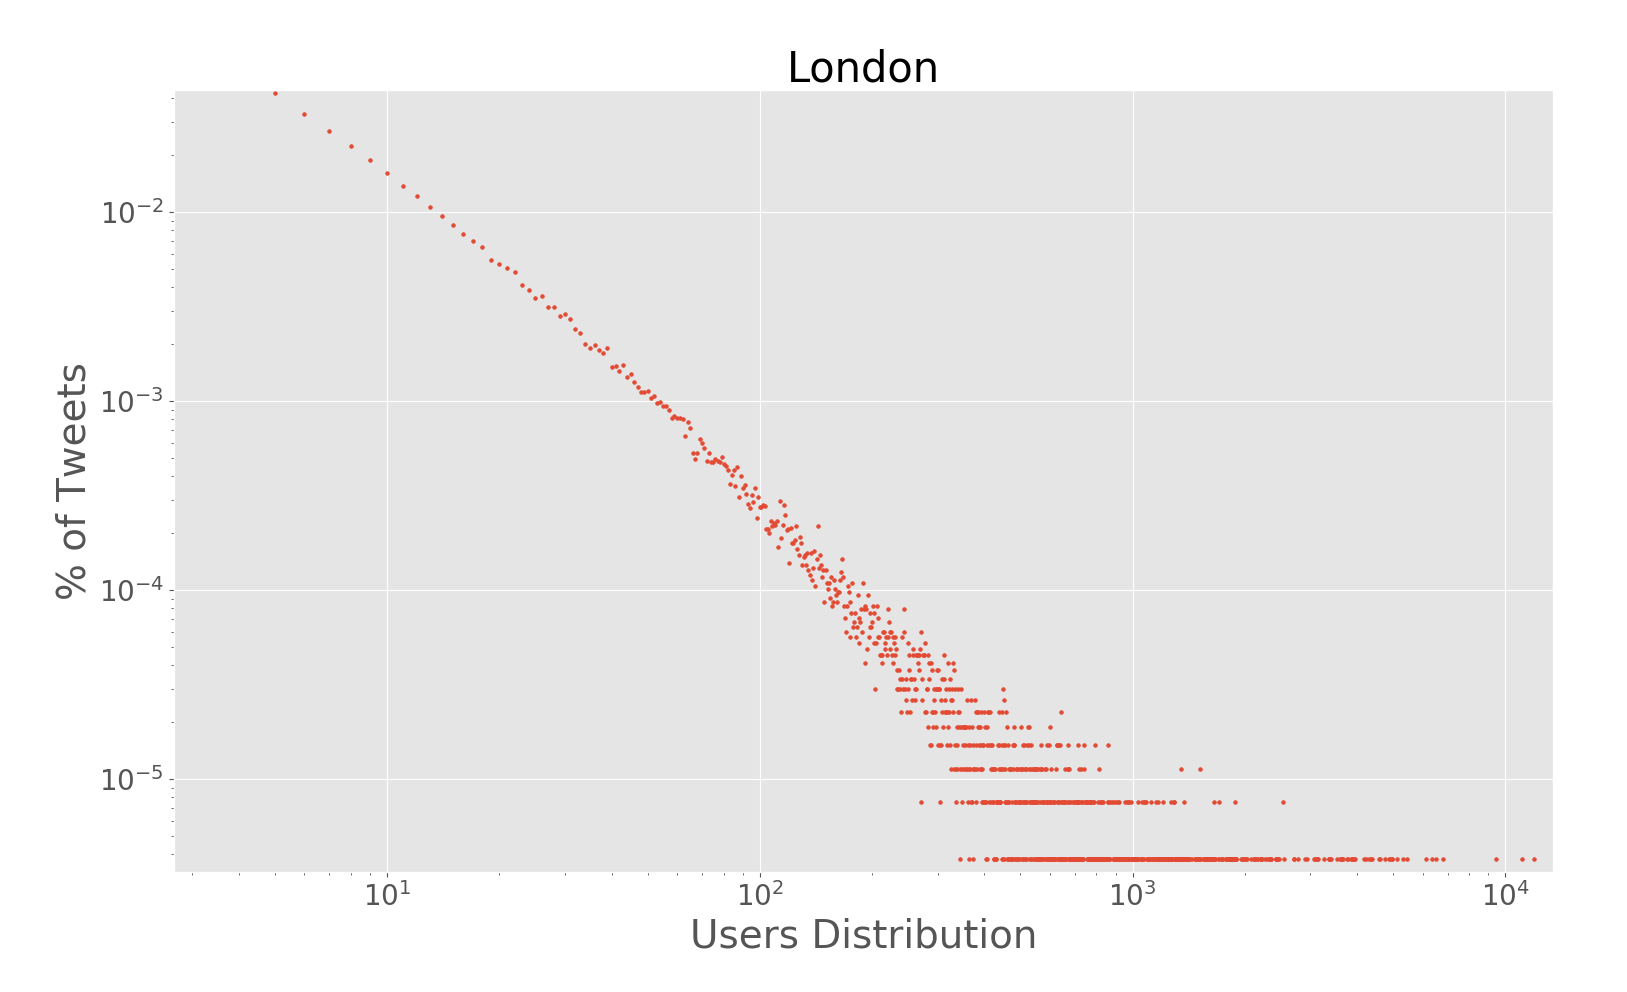
\includegraphics[width=1\linewidth]{figures/london_loglog_users.png}
		\caption{}
		\label{subfig:london_loglog_users}
	\end{subfigure}
	
	\medskip
	
	\begin{subfigure}[t]{0.45\textwidth}
		\centering
		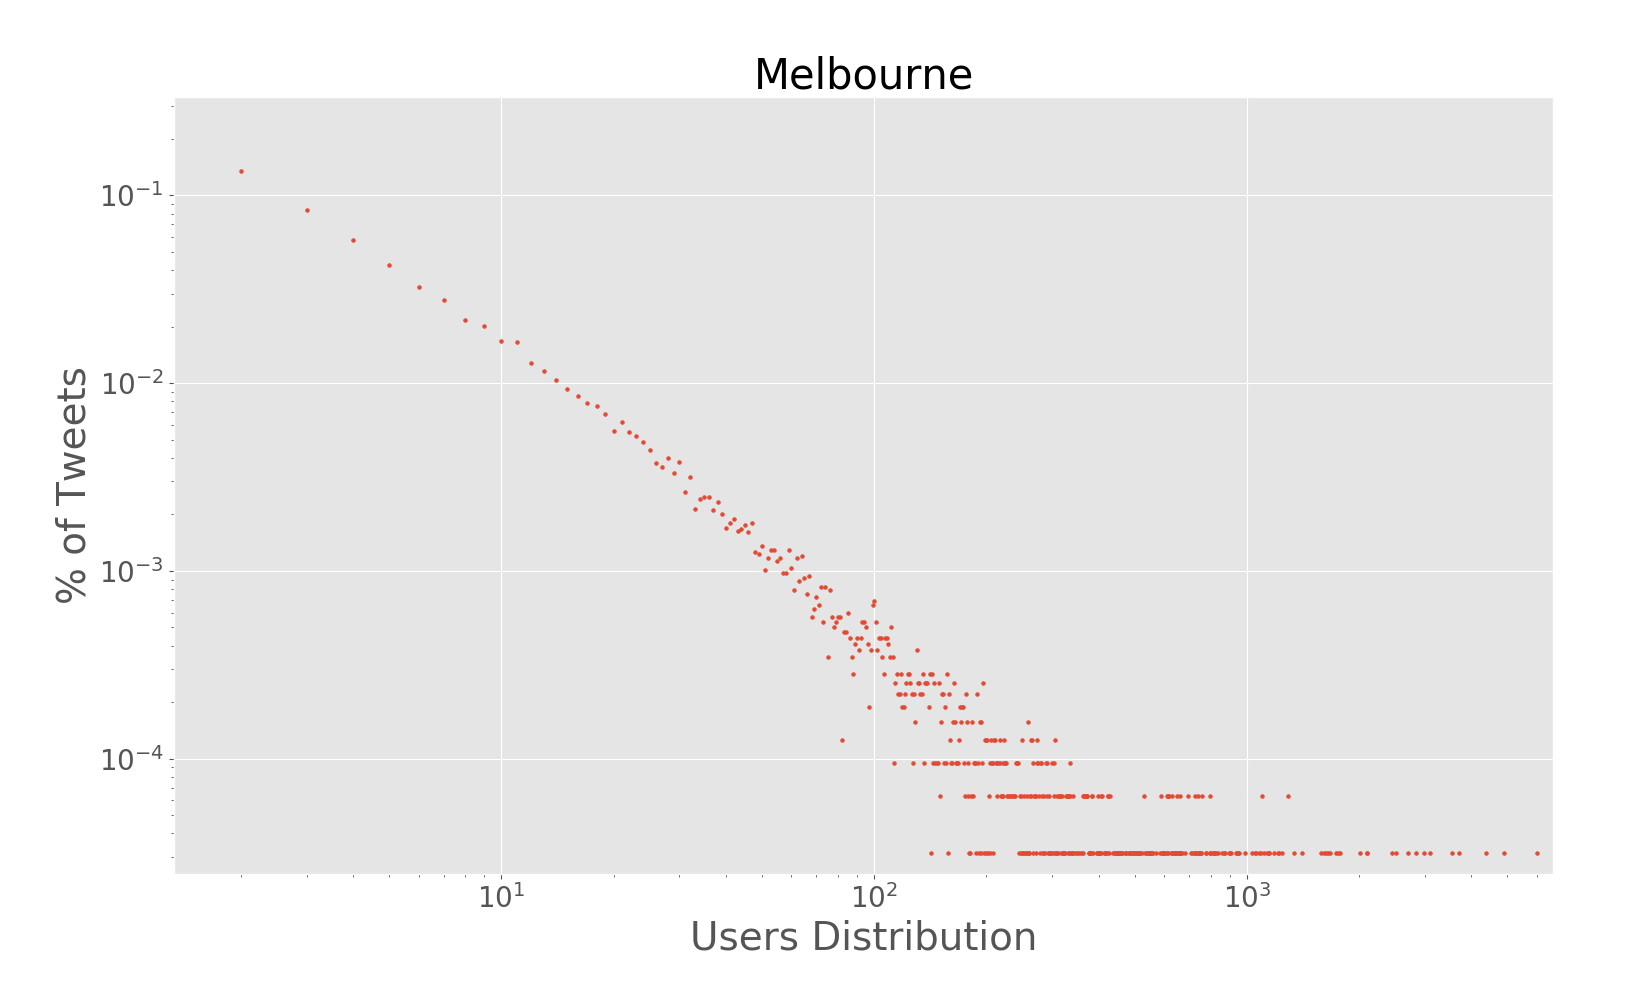
\includegraphics[width=1\linewidth]{figures/melbourne_loglog_users.png}
		\caption{}
		\label{subfig:melbourne_loglog_users}
	\end{subfigure}
	
	\caption[Five numerical solutions]{Log-log plots for the users distribution over the number of tweets posted (a) Rio de Janeiro (b) São Paulo (c) New York City (d) London (e) Melbourne}
	\label{fig:loglog-plots-users}
\end{figure}

The last analysis presented in this subsection is related to the \textit{metadata} contained in the tweets. Here, we want to characterize the different cities with respect to the amount of extra content used by the users in the posts and what kind of information such results suggests for each city.

Having this considered, we counted the volume of each element constituting the previously mentioned \textit{metadata} and calculate the percentage of tweets containing it. In Table~\ref{tab:metadata} are listed the counts and the corresponding percentage of it relatively to the datasets. The resulting analysis and results were performed over the tweets with the city's native language and located inside the bounding-box area used in the filtering process.
The most observable evidence in the results is the greater use of this elements in the English speaking cities. User mentions, as well as \textit{URLs} are the most used \textit{metadata}. This elements may suggest that citizens tend to tag other people in their messages when posting and also share information about certain topic through urls. Regarding the Brazilian cities, the \textit{metadata} usage is not so noticeable. This fact may me related to the number of users composing each dataset because, as it was previously mentioned, the English speaking cities possesses almost two times more users than the Brazilian cities and this characteristic contributes to the increase of this type of \textit{metadata} usage since when someone tag another one in a message, usually a re-post is sent tagging the person responsible by the starting of the conversation. To prove this so, an intensive study about social media tracking and mapping of the flow of each Twitter conversation is needed.

\begin{table}[htbp]
	\centering
	\caption{Percentage of Metadata composing the datasets}
	\label{tab:metadata}
	\resizebox{\textwidth}{!}{\begin{tabular}{l|c|cc|cc|cc|cc}
		\hline
		\multicolumn{1}{c|}{\multirow{2}{*}{\textbf{City}}} & \multicolumn{1}{l|}{\multirow{2}{*}{\textbf{Total}}} & \multicolumn{2}{c|}{\textbf{Hashtags (\#)}} & \multicolumn{2}{c|}{\textbf{User Mentions (@)}} & \multicolumn{2}{c|}{\textbf{URLs}} & \multicolumn{2}{c|}{\textbf{Media}} \\ \cline{3-10} 
		\multicolumn{1}{c|}{} & \multicolumn{1}{l|}{} & \multicolumn{1}{c|}{\textbf{Total (tweets)}} & \textbf{\%} & \multicolumn{1}{c|}{\textbf{Total (tweets)}} & \textbf{\%} & \multicolumn{1}{c|}{\textbf{Total(tweets)}} & \textbf{\%} & \multicolumn{1}{c|}{\textbf{Total (tweets)}} & \textbf{\%} \\ \hline
		\textbf{Rio de Janeiro} & 11,060,136 & 504,835 & 4,56\% & 1,336,329 & 12,08\% & 1,783,060 & 16,12\% & 409,500 & 3,70\% \\
		\textbf{São Paulo} & 4,886,626 & 593,952 & 12,15\% & 1,030,341 & 21,08\% & 1,111,749 & 22,75\% & 325,385 & 6,66\% \\
		\textbf{New York City} & 5,956,355 & 1,697,416 & 28,50\% & 1,752,839 & 29,43\% & 2,839,794 & 47,68\% & 535,945 & 9,00\% \\
		\textbf{London} & 4,040,092 & 1,163,981 & 28,81\% & 1,744,051 & 43,17\% & 1,812,152 & 44,85\% & 465,610 & 11,52\% \\
		\textbf{Melbourne} & 629,424 & 195,967 & 31,13\% & 271,970 & 43,21\% & 258,278 & 41,03\% & 65,941 & 10,48\% \\ \hline
	\end{tabular}}
\end{table}

\subsection{Final Remarks}
In this section we tried to identify interesting patterns and valuable information recurring only to the simple characteristics provided by a tweet, location, date of creation and \textit{metadata} content. First, it was possible to find out existing problems regarding the collection of geo-located tweets. More than one problem is mentioned and possible solutions were designed to surpass them. Our datasets represent only three months of data, however supporting in the analysis made, we conclude that the majority of tweets are tagged with variable sized bounding-boxes instead of precisely geo-coordinates. Furthermore, we tried to instigate temporal patterns using the, already, filtered tweets and proved that it is possible to learnt about remarkable events only seeing abrupt activity on Twitter for some days. By studying the Twitter users distribution it was possible correlate the behaviour of it with the famous power-law distribution. Last but not least, a brief analysis of the \textit{metadata} was performed in order to see the amount of possible topics identified on it (hashtags), the volume of tweets mentioning another user and how many information can be share through the use of urls in this microblog, named Twitter.

%The methodology reported across this experiment is concerned with topic modelling over two datasets from two Brazilian cities in order to characterize the topics that people talked about and compare the results in both scenarios. LDA models usually requires documents of large size, or at least more complex than a single tweet, in order to get good performance. A traditional approach was followed considering each tweet as a document instead of trying aggregate tweets in more complex documents taking into consideration some criteria, e.g. grouping by date and hour. The final results showed that topics in both cities are very similar and only two of them are unique. With exception of topics - \textit{Relationships and Friendship} and \textit{Personal Feelings}, the percentage difference between similar topics was comprehended in the interval 0.16-4.43\% evidencing the fact that both cities are similar besides the different factors that characterize each one: population, culture, lifestyle and also the region where the city is located in. Although all this analysis, we can not assure that inside a topic we do not have more topics hidden. Our classification was limited to the verification of the 50 top words and the manually verification of a sample of 200 tweets since the resulting amount of tweets for each topic is impossible to verify one by one. Due to this, another classification approach need to be explored and a promising one was proposed by D. Ramage et al.~\cite{ramage2010characterizing}. The classification will be automatic by adding a supervised extra layer to the pipeline. However, to assure trustiness in the results the data may be manually labelled for the training phase of the model classification or, at least, have reliable sources, for example, exploring the topics provide by the Wikipedia articles\footnote{\url{https://dumps.wikimedia.org/ptwiki/20170601/}}.

\section{Topic Modelling}\label{sec:topic_modeling}
This section is related to the experiment of automatically characterize tweets in two different Brazilian cities, Rio de Janeiro and São Paulo. We used an unsupervised learning approach to tackle the task of topic modelling in order to compare both cities and see if there are differences between subjects people talked about. Automatic characterization of text messages is a laborious and time consuming task since it is necessary to assure the right level of abstraction in the learning model; very much similarly to human minds, which essentially present a bounded rationality nature, our learning model needs to be trained in order to assimilate the necessary knowledge and perform the appropriate analogies so as to discover different topics within the tweets' contents. The premises to implement such a mechanism are presented and discussed in the following subsections.

\subsection{Data Selection}
The data selected to conduct this experiment is correspondent to a period of two months, between days March 12 and May 12, 2017. 

The resulting datasets sum up a total of 12.5M and 6.3M tweets for Rio de Janeiro and for São Paulo, respectively. Due to the problem detected in Section~\ref{sec:data_collection}, we filtered the data in order to only use the tweets that were actually inside the cities' areas. The final composition of the datasets is presented in Table~\ref{tab:datasets}, and the results of the filtering process shown that almost 6M tweets were not located inside the bounding-boxes of the cities.

\begin{table*}[ht]
\small
\centering
\caption{Datasets composition}
\label{tab:datasets}
\resizebox{\textwidth}{!}{\begin{tabular}{|c|c|c|c|c|c|c|}
\hline
\textbf{City}  & \textbf{All} & \textbf{PT} & \textbf{Non-PT} & \textbf{\begin{tabular}[c]{@{}c@{}}In \\ Bounding-Box\end{tabular}} & \textbf{\begin{tabular}[c]{@{}c@{}}Out\\ Bounding-Box\end{tabular}} & \textbf{\begin{tabular}[c]{@{}c@{}}PT and \\ In Bounding-Box\end{tabular}} \\ \hline
Rio de Janeiro & 12,531,000 & 10,570,000 & 1,961,000 & 8,644,000 & 3,886,000 & 7,353,000 \\ \hline
São Paulo & 6,352,000 & 4,886,000 & 1,466,000 & 4,247,000 & 2,105,000 & 3,313,000 \\ \hline
\end{tabular}}
\end{table*}

The subset of data composed by Portuguese tweets and located inside the cities' bounding-boxes was used to conduct the experiment described in this section. Such subset can be sum up to a total of 7.3M and 3.3M for Rio de Janeiro and São Paulo, respectively.

\subsection{Data Preparation}
Usually, to tackle topic modelling tasks in text documents it is required several pre-processing steps. Such pre-processing to the data helps the operations made by the LDA model, which is the technique used here. Removing unnecessary words, transforming words into their root form as so deleting all the punctuation are some of the common text mining pre-processing steps. Here, each tweet of both datasets was submitted to a required group of pre-processing operations in order to train a LDA model and proceed with the experiments. The pre-processing steps were the ones detailed below.

\begin{itemize}
\item \textbf{Lowercasing:} Every message presented in a tweet was converted into lower case;
\item \textbf{Cleaning Entities and Numbers:} Removing \textit{URLs}, user mentions, \textit{hashtags} and digits from the text message;
\item \textbf{Lemmatization:} Only plural words were transformed into singular ones;
\item \textbf{Transforming repeated characters:} Sequences of characters repeated more than three times were transformed, e.g. "loooool" was converted to "loool";
\item \textbf{Punctuation Removal:} Every punctuation was removed as well as smiles (e.g. \texttt{:)}, \texttt{:-)}, \texttt{=D}) or even \emph{emoticons};
\item \textbf{Stop Words Removal:} The removing of this kind of words was made using the Portuguese NLTK dictionary;
\item \textbf{Short Tokens Removal:} Words such as 'kkk', 'aaa', 'aff' and other of the same style were removed.
\end{itemize}

After the data preparation phase, 772,017 tweets have their message empty which conclude that its content was irrelevant for the final experiment phase.

\subsection{Features Selection}
Topic modelling requires, like in other learning model, a group of features to be trained. In this case, we used the Bag-of-Words representation matrix - which is a representation where each document is converted to a frequency vector according to the number of occurrences of each word in the message. The set of features was limit to a dictionary containing 10,000 words and it only took into account uni-grams in the message content. The dictionary was also limited to words that occur in a maximum percentage of 40$\%$ in the whole dataset, avoiding common words that were not removed because they were not included in the NLTK Stop Words list. The minimal occurrence value for a word being considered was set to 10.

\subsection{LDA Model Parametrization}
In order to understand and see the LDA model performance, we set five different numbers for the topics results parameter of the training process: 5, 10, 20, 25 and 50 topics, being this the one with better results. The number of iterations to train the model was set to 20, since our desired was to reproduce the experiment made by G. Lansley et al.~\cite{lansley2016geography} to the city of London. Finally but not the least, each tweet in the datasets was treated as a single document comprehending that, in total, 6,580,983 different documents were used in the model training process. The complete pipeline according to all the steps taken to conduct this experiment is observable in Figure~\ref{fig:pipeline_lda}.

\begin{figure}[h]
\centering
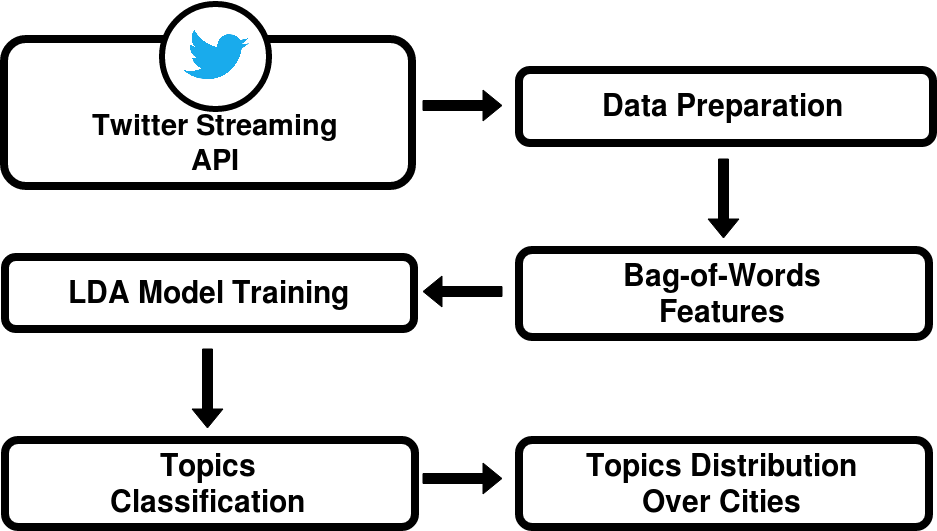
\includegraphics[width=0.6\linewidth]{figures/pipeline_lda.png}
\caption{Correspondent pipeline of the topic modelling experiment}
\label{fig:pipeline_lda}
\end{figure}

\subsection{Results and Analysis}
To evaluate the experimental results obtained for each model (where the difference underlies on the variation of the number of topics), a list with the most frequent 50 words for each topic was extracted. In Table~\ref{tab:topics_classification} we can observe a sample (20 top words) selected out of the 50 studied. Nonetheless, the final evaluation takes into consideration the 50 frequent words.

\begin{table}[h]
\centering
\caption{Example of the topics classification}
\label{tab:topics_classification}
\resizebox{\textwidth}{!}{\begin{tabular}{c|c}
\hline
\textbf{\begin{tabular}[c]{@{}c@{}}Words\\ (only 20 words)\end{tabular}} & \textbf{\begin{tabular}[c]{@{}c@{}}Topic\\ Classification\end{tabular}} \\ \hline
\begin{tabular}[c]{@{}c@{}}paulo, vai, hoje, dia, jogo, ser, melhor, time, vamo, brazil, \\ todo, santo, brasil, gol, cara, aqui, agora, corinthiam, ano, palmeiro, vem, ...\end{tabular} & \begin{tabular}[c]{@{}c@{}}Sports and\\ Games\end{tabular} \\ \hline
\begin{tabular}[c]{@{}c@{}}vou, dia, dormir, queria, hoje, ficar, casa, semano, quero, ter, \\ ainda, hora, agora, sono, aula, acordar, acordei, cedo, fazer, prova, ...\end{tabular} & \begin{tabular}[c]{@{}c@{}}Wake-up\\ Messages\end{tabular} \\ \hline
\begin{tabular}[c]{@{}c@{}}top, social, artist, vote, the, award, army, bom, voting, doi, \\ bogo, oitenta, sipda, today, vinte, prepara, cypher, oito, quatro, man, ...\end{tabular} & \begin{tabular}[c]{@{}c@{}}Voting and\\ Numbers\end{tabular} \\ \hline
\begin{tabular}[c]{@{}c@{}}marco, nada, falar, emilly, gente, quer, nao, pessoa, nunca, fala, \\ vai, falando, sobre, chama, agora, manda, vem, mensagem, vivian, bbb, ...\end{tabular} & \begin{tabular}[c]{@{}c@{}}Big Brother\\ Brazil 2017\end{tabular} \\ \hline
\begin{tabular}[c]{@{}c@{}}paulo, brazil, sao, santo, vila, just, parque, posted, photo, shopping, \\ paulista, centro, bernardo, jardim, cidade, avenido, praia, santa, campo, academia\end{tabular} & \begin{tabular}[c]{@{}c@{}}Tourism and\\ Places\end{tabular} \\ \hline
\end{tabular}}
\end{table}

We also selected and manually analyse a random sample (with the size of 200) of tweets for each topic. This sampling was done in order to get better consistency and trustiness about the classification and characterization of the tweets.

It was found a group of 50 topics which had the largest number of distinct topics between them. However, there were topics which theme was the same (e.g. Love and Romance Problems or Brazilian Football \textit{versus} European Football). Within this, such groups were aggregate into the same topic, \textit{Relationships} and \textit{Sports and Games}, respectively. After this grouping process, a total of 29 different topics was achieved. 

Some tweets that have added complexity to our classification objective, such as, for example, "\textit{queria namorar um mano parecido com o josh}" (Relationship) and "\textit{como eu queria meus amigos aqui agora cmg}" (Friendship), raised some doubts about which topic this tweets may belong: Relationship, Friendship or even Actions or Intentions. In a perspective of context, the first tweet belongs to the theme \texttt{flirt}, which is directly related to Relationship. The theme on the second tweet is missing the company of friends, i.e. conviviality, which is related to Friendship. The decision of join the two topics was due to the proximity between them which have as content both types of tweets, talking about love/relationship and friendship, and with this in consideration both topics should be aggregated in order to assure the desired consistency in the classification.

The final set of topics (50 topics) to be considered was selected accordantly to the most recurring subjects. The final classification and details associated with the whole dataset for each city is presented in Table~\ref{tab:final_classification}. Almost every topics demonstrated a balanced distribution, with exception of \textit{Relationships and Friendship} and \textit{Personal Feelings} for Rio de Janeiro and São Paulo, respectively. The difference that appear in this topics is a consequence of the final grouping process, since there was a considerable number of words been shared among this topics. This issue complicated our classification task, compelling to an high amount of undesired aggregations.

\begin{table}[ht]
\small
\caption{Final results of the LDA topics aggregation}
\label{tab:final_classification}
\resizebox{\textwidth}{!}{\begin{tabular}{l|cc|cc|c}
\hline
\multicolumn{1}{c|}{\multirow{2}{*}{\textbf{Topic Group}}} & \multicolumn{2}{c|}{\textbf{Rio de Janeiro}} & \multicolumn{2}{c|}{\textbf{São Paulo}} & \multicolumn{1}{c|}{\multirow{2}{*}{\textbf{Diff (\%)}}} \\ \cline{2-5}
\multicolumn{1}{c|}{} & \textbf{No. Tweets} & \textbf{Percentage (\%)} & \textbf{No. Tweets} & \textbf{Percentage (\%)} & \multicolumn{1}{c|}{} \\ \hline
Academic Activities & 101,590 & 1,54\% & 90,616 & 3,30\% & -1,76\% \\
Actions or Intentions & 600,030 & 9,12\% & 128,710 & 4,69\% & \textbf{+4,43\%} \\
Antecipation and Socialising & 132,606 & 2,01\% & 0 & 0,00\% & \textbf{+2,01\%} \\
BBB17 & 122,054 & 1,85\% & 68,385 & 2,49\% & -0,64\% \\
Body, Appearances and Clothes & 160,342 & 2,44\% & 71,447 & 2,60\% & -0,17\% \\
Food and Drink & 167,204 & 2,54\% & 58,407 & 2,13\% & +0,41\% \\
Health & 119,013 & 1,81\% & 0 & 0,00\% & \textbf{+1,81\%} \\
Holidays and Weekends & 104,695 & 1,59\% & 79,610 & 2,90\% & -1,31\% \\
Informal Conversations & 272,502 & 4,14\% & 138,848 & 5,06\% & -0,92\% \\
Live Shows, Social Events and Nightlife & 359,342 & 5,46\% & 140,240 & 5,11\% & +0,35\% \\
Mood & 139,287 & 2,12\% & 138,399 & 5,04\% & \textbf{-2,92\%} \\
Movies and TV & 285,198 & 4,33\% & 39,778 & 1,45\% & \textbf{+2,89\%} \\
Music and Artists & 84,407 & 1,28\% & 78,142 & 2,85\% & 1,56\% \\
Negativism, Pessimism and Anger & 229,104 & 3,48\% & 183,050 & 6,67\% & \textbf{-3,18\%} \\
Numbers, Quantities and Classification & 86,897 & 1,32\% & 78,160 & 2,85\% & -1,53\% \\
Optimism and Positivism & 106,714 & 1,62\% & 39,725 & 1,45\% & +0,18\% \\
Personal Fellings & 375,735 & 5,71\% & 532,331 & 19,38\% & \textbf{-13,67\%} \\
Politics & 81,254 & 1,23\% & 46,758 & 1,70\% & 0,47\% \\
Relationships and Friendship & 1,524,804 & 23,17\% & 187,541 & 6,83\% & \textbf{+16,34\%} \\
Religion & 183,174 & 2,78\% & 66,788 & 2,43\% & +0,35\% \\
Routine Activities & 334,216 & 5,08\% & 82,421 & 3,00\% & +2,08\% \\
Slang and Profinities & 241,676 & 3,67\% & 44,620 & 1,62\% & +2,05\% \\
Social Media Applications & 105,809 & 1,61\% & 44,073 & 1,60\% & +0,01\% \\
Sport and Games & 382,479 & 5,81\% & 133,047 & 4,84\% & +0,97\% \\
Tourism and Places & 59,288 & 0,90\% & 86,519 & 3,15\% & -2,25\% \\
Transportation and Travel & 130,261 & 1,98\% & 63,923 & 2,33\% & -0,35\% \\
Weather & 91,302 & 1,39\% & 42,588 & 1,55\% & -0,16\% \\
Shopping & 0 & 0,00\% & 44,470 & 1,62\% & \textbf{-1,62\%} \\
Voting & 0 & 0,00\% & 37,687 & 1,37\% & \textbf{-1,37\%} \\ \hline
\end{tabular}}
\end{table}

Additionally to the manual verification of a sample of tweets for each topic, we also produced a temporal week day distribution,  with the objective to observe if some topics had more mentions in certain days than others.

For making such observations some assumptions were made in relation with some \textit{hot} topics. More specifically, we think that is valid to assume that people will talk more about \textit{Religion} in the weekend, since they go to the church in those days. The same result is likely to happen for topics like \textit{Holidays and Weekends} or \textit{Sports and Games}, since events related to this thematics occur during specific time-frames. 

Only 12 topics of the finals 29 were selected for this part of the study, predicting them and comparing the final results, such as, but not limited to, \textit{Sports and Games}, \textit{Religion}, \textit{Holidays and Weekends}, \textit{Movies and TV}, \textit{Live Shows, Social Events and Nightlife}. The temporal distribution is showed in Figure~\ref{fig:topics_heat_maps} as a heat map, where each row is independent from the others.

The necessity of applying such restrictions is due to the need of seeing in which days each topic is more talked about. For both cities the topic \textit{Sports and Games} is more mentioned in Tuesdays and Saturdays. Indeed, this observation correlates with the days that topic-related events happens. Namely, Tuesdays and Wednesday correspond to the days when the \textit{UEFA Champions League} competition happens and Saturdays and Sundays to the days of \textit{Brazilian Football League} games. \textit{Holidays and Weekends} was a topic with interesting results regarding the temporal distribution, presenting Sundays as the day where more people talk about it. 

Furthermore, it is worth mentioning that our model had successfully discover a topic related to Big Brother Brazil 2017 (BBB17), a well-known reality show. The amount of geo-located tweets concerning this topic was considerable (1.85\% and 2.49\%, in RJ and SP, respectively), rising the question about what led people to geo-located them in such topic.

\begin{figure}[h]
\centering
\begin{subfigure}{0.49\textwidth}
\centering
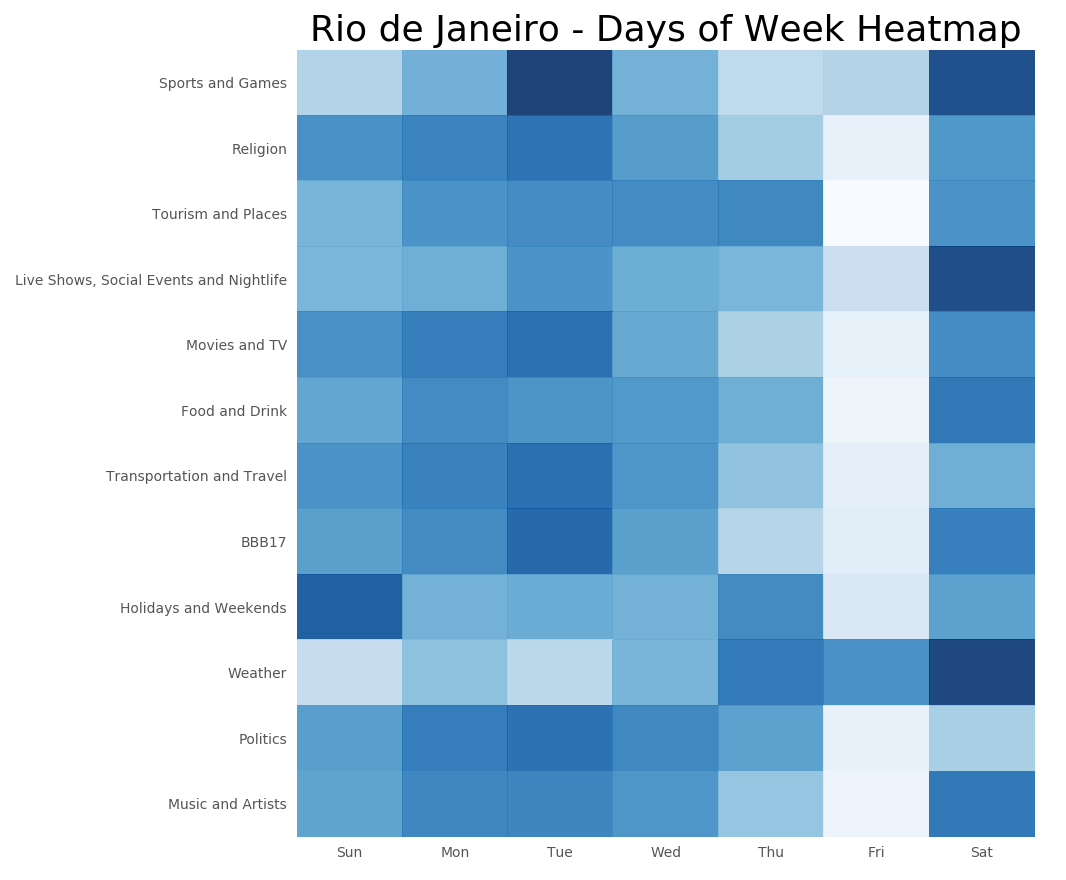
\includegraphics[width=1.0\linewidth]{figures/rio_topics_heatmap.png}
\label{fig:rio}
\end{subfigure}
\begin{subfigure}{0.49\textwidth}
\centering
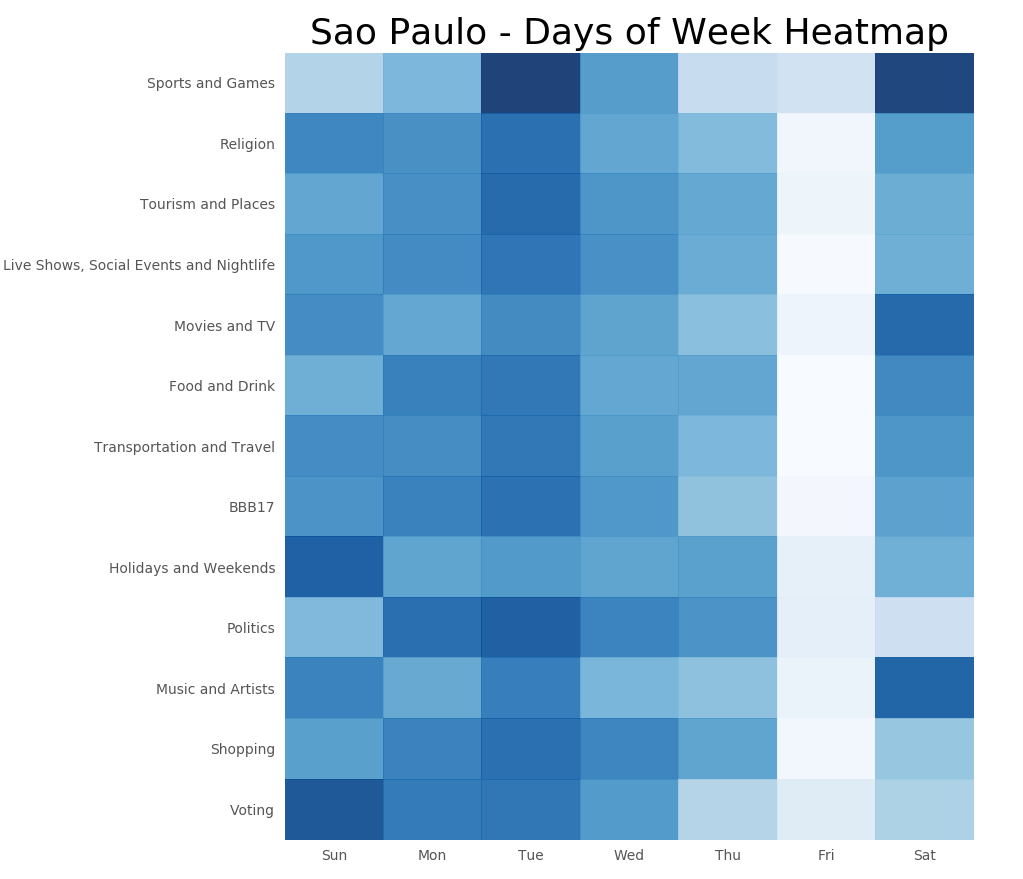
\includegraphics[width=1.0\linewidth]{figures/sp_topics_heatmap.png}
\label{fig:sp}
\end{subfigure}
\caption{Day-of-the-week activity per each topic in both cities, Rio de Janeiro and São Paulo}
\label{fig:topics_heat_maps}
\end{figure}

\subsection{Final Remarks}
The methodology reported across this experiment is concerned with topic modelling over two datasets from two Brazilian cities in order to characterize the topics that people talked about and compare the results in both scenarios. LDA models usually requires documents of large size, or at least more complex than a single tweet, in order to get good performance. A traditional approach was followed considering each tweet as a document instead of trying aggregate tweets in more complex documents taking into consideration some criteria, e.g. grouping by date and hour. The final results showed that topics in both cities are very similar and only two of them are unique. With exception of topics - \textit{Relationships and Friendship} and \textit{Personal Feelings}, the percentage difference between similar topics was comprehended in the interval 0.16-4.43\% evidencing the fact that both cities are similar besides the different factors that characterize each one: population, culture, lifestyle and also the region where the city is located in. Although all this analysis, we can not assure that inside a topic we do not have more topics hidden. Our classification was limited to the verification of the 50 top words and the manually verification of a sample of 200 tweets since the resulting amount of tweets for each topic is impossible to verify one by one. Due to this, another classification approach need to be explored and a promising one was proposed by D. Ramage et al.~\cite{ramage2010characterizing}. The classification will be automatic by adding a supervised extra layer to the pipeline. However, to assure trustiness in the results the data may be manually labelled for the training phase of the model classification or, at least, have reliable sources, for example, exploring the topics provide by the Wikipedia articles\footnote{\url{https://dumps.wikimedia.org/ptwiki/20170601/}}.

\section{Portuguese Travel-related Classification}\label{sec:travel_related_classification}
The main goal of this section is to detail the experiment that supports the characterization of travel-related tweets in Rio de Janeiro and São Paulo. Considering the volume of the collected data, it was then necessary to automatically identify tweets whose content somehow suggests to be related to the transportation domain. Conventional approaches would require us to specify travel-related keywords to classify such tweets. On the contrary, our approach consisted in training a classifier model to automatically discriminate travel-related tweets from non-related ones. 

One big challenge always present in text analysis is the sparse nature of data, which is especially the case in Twitter messages.
Conventional techniques such as Bag-of-Words tend to produce sparse representations, which become even worse when data is composed by informal and noisy content.

Word embeddings, on the other hand, is a text representation technique that tries to capture syntactic and semantic relations from words. The result is a more cohesive representation where similar words are represented by similar vectors. For instance, \emph{"taxi"/"uber"}, \emph{"bus/busão/ônibus"}, \emph{"go to work"/"go to school"} would yield similar vectors respectively.
We are particularly interested in exploring the characteristics of word embeddings techniques to understand which extent it is possible to improve the performance of our classifier to capture such travel-related expressions. In the following subsections, we describe the necessary steps to build our classification model.

\subsection{Data Selection}
Messages were collected for a period of one whole month, between days March 12 and April 12, 2017, and the resulting datasets sum up a total of 6.1M and 2.9M tweets for Rio de Janeiro and São Paulo, respectively. Due to the problem detected in Section~\ref{subsec:geographical_distribution}, we filtered the data in order to only use the tweets that were actually inside the cities' areas. The final composition of the datasets is presented in Table~\ref{tab:brazilian_datasets_travel}, and according the previous mentioned criteria, a sum up of 7.7M tweets (5.3M and 2.4M tweets for Rio de Janeiro and São Paulo, respectively) was considered in this experiment.

\begin{table}[ht]
	\small
	\centering
	\caption{Rio de Janeiro and São Paulo datasets composition for the travel-related classification}
	\label{tab:brazilian_datasets_travel}
	\resizebox{\textwidth}{!}{\begin{tabular}{|c|c|c|c|c|c|c|}
			\hline
			\textbf{City}  & \textbf{All} & \textbf{PT} & \textbf{Non-PT} & \textbf{\begin{tabular}[c]{@{}c@{}}Inside \\ Bounding-Box\end{tabular}} & \textbf{\begin{tabular}[c]{@{}c@{}}Outside\\ Bounding-Box\end{tabular}} & \textbf{\begin{tabular}[c]{@{}c@{}}PT and Inside \\ Bounding-Box\end{tabular}} \\ \hline
			Rio de Janeiro & 6,175,000 & 5,355,000 & 0,819,000 & 4,327,000 & 1,848,000 & 3,749,000 \\ \hline
			São Paulo      & 2,934,000 & 2,444,000 & 0,490,000 & 2,016,000 & 0,918,000 & 1,672,000 \\ \hline
		\end{tabular}}
	\end{table}

\subsection{Data Preparation}
Each tweet of our training and test sets was submitted to a small and basic group of pre-processing operations, as detailed below.

\begin{itemize}
\item \textbf{Lowercasing:} Every message presented in a tweet was converted into lower case;
\item \textbf{Transforming repeated characters:} Sequences of characters repeated more than three times were transformed, e.g. "loooool" was converted to "loool";
\item \textbf{Cleaning:} URLs and user mentions were removed from the text.
\end{itemize}

\subsection{Features Selection}\label{features_4_3_2}
We established the use of different groups of features to train our classification model, namely bag-of-words, bag-of-embeddings - word embeddings dependent technique - and both combined. Such groups are detailed below.

\begin{itemize}
\item \textbf{Bag-of-words (BoW):} This group of features was obtained using unigrams with standard bag-of-words techniques. We considered the 3,000 most frequent terms across the training set excluding the ones found in more than 60$\%$ of the documents (tweets);

\item \textbf{Bag-of-embeddings (BoE):} We applied bag-of-embeddings to each tweet using a \textit{doc2vec} model~\footnote{\url{https://radimrehurek.com/gensim/models/doc2vec.html} (Accessed on 09/06/2017)} combining Deep Learning and \textit{paragraph2vec}. The model was trained with 10 iterations over the whole Portuguese dataset using a context window of value 2 and feature vectors of 100 dimensions. We then took the corresponding embedding matrix to yield the group of features fed into our classification routine. 

\item \textbf{Bag-of-words plus Bag-of-embeddings:} We horizontally combined both the above matrices into a single one and used it as a single group of features.
\end{itemize}

\subsection{Training and Test Datasets}\label{subsec:training_test_datasets_portuguese}
The construction of the training and test sets followed a traditional approach. We thus tried to select balanced training sets, to which it was necessary to identify tweets that could possibly be travel-related. We were inspired by a strategy used in the study by Maghrebi~et~al.~\cite{maghrebi2016transportation}, which consists in searching tweets from a collection using specific travel terms and regular expressions.

Using the terms declared in Table~\ref{tab:terms} combined with the regular expression $space + term + space$, we found about 30,000 tweets. From this subset, we randomly selected a small sample of 3,000 tweets to manually confirm if they were indeed related to travel topics. After this manual annotation we selected 2,000 tweets and used them as positive samples in the training dataset.

In order to select negative samples for the training dataset we randomly selected 2,000 tweets and also manually verified their content to assure that they were not travel-related. Finally, our training set was composed by 4,000 tweets, from which 2,000 were travel-related and 2,000 were not. 
We selected 1,000 tweets randomly that were not present in the training set to build the test set, and then manually classified them as travel-related or non-travel-related. In the end, 71 tweets were found to be travel-related and whereas 929 were not.

\begin{table}[htbp]
	\centering
	\small
	\caption{Travel terms used to build the training set}
	\label{tab:terms}
	\begin{tabular}{c|c|c}
		\hline
		\multirow{2}{*}{\textbf{Mode of Transport}} & \multicolumn{2}{c|}{\textbf{Terms}} \\ \cline{2-3} 
		& \multicolumn{1}{l|}{\textbf{Portuguese Language}} & \textbf{English Language} \\ \hline
		\textbf{Bike} & bicicleta, moto & bicycle, bike \\
		\textbf{Bus} & onibus, ônibus & bus \\
		\textbf{Car} & carro & car \\
		\textbf{Taxi} & taxi, táxi & taxi, cab \\
		\textbf{Train} & metro, metrô, trem & metro, train, subway \\
		\textbf{Walk} & caminhar & walk \\ \hline
	\end{tabular}
\end{table}

\subsection{Estimators and Evaluation Metrics}
Support Vector Machines (SVM), Logistic Regression (LR) and Random Forests (RF) were the classifiers used in our experiments. The SVM classifier was tested under three different kernels, namely \textit{rbf}, \textit{sigmoid} and \textit{linear}; the latter proved to obtain the best results. 

The LR classifier was used with the standard parameters, whereas the RF classifier used 100 trees in the forest. The gini criterion and the maximum number of features were limited to those as aforementioned in Section~\ref{features_4_3_2}, in the case of the RF classifier.

To evaluate the performance of the classifiers in our experiences we used five different metrics. Firstly we compute a group of three per-class metrics, namely precision, recall and the F1-score. Bearing in mind this study considers a binary classification, metrics were associated with the travel-related class only, i.e. the positive class. Therefore, the interpretation for each metric is provided below:

\begin{itemize}
\item \textbf{Precison:} Represents the fraction of correct predictions for the travel-related class (Equation~\ref{eq:precision}).

\item \textbf{Recall:} Represents the fraction of travel-related tweets correctly predicted (Equation~\ref{eq:recall}).
\begin{multicols}{2}
	\begin{equation}\label{eq:precision}
		Precision = \frac{tp}{tp+fp}
    \end{equation}
    
	\begin{equation}\label{eq:recall}
		Recall = \frac{tp}{tp+fn}
	\end{equation}
\end{multicols}

where \textbf{$tp$} is related to the true positives classified tweets, \textbf{$fp$} represents the false positives and \textbf{$fn$} are the false negatives.

\item \textbf{F1-score:} Represents the harmonic mean of precision and recall.
\end{itemize}

\begin{equation}
{F1}_{score} = 2*\frac{precision*recall}{precision+recall}
\end{equation}

Once these first three metrics only showed us the performance of the classifier for a discrimination threshold of 0.5, we decided to calculate another metric. The ROC (Receiver operating characteristic) curve gives us the TPR (True positive rate) and the FPR (False positive rate) for all possible variations of the discrimination threshold. Through the ROC curve, we compute the area under the curve (AUC) to see what was the probability of the classifier to rank a random travel-related tweet higher than a random non-related one.

\subsection{Results and Analysis}
Table~\ref{classifiers} presents the results obtained using the different features combination for our test set composed by 1,000 tweets manually annotated. According to the evaluation metrics we conclude that the bag-of-word and bag-of-embeddings combined produced better classification models. The model produced by the Linear SVM performed slightly better than the LR and the RF. Interesting to note is that BoW features have influence on the precision scores obtained from our results, producing more conservative classifiers. Regarding the recall results, we can see that the Logistic Regression using only bag-of-embeddings features was the model with best results; perhaps if the precision is taken into consideration, the same conclusions will not be possible. Analysing the scores provided in Table~\ref{classifiers}, the best model under the F1-score was the Linear SVM, with a score of 0.85.

\begin{table}[!htbp]
\footnotesize
\centering
\caption{Classifiers Experiences}
\label{classifiers}
\begin{tabular}{|c|c|c|c|c|}
\hline
\textbf{Classifier}                  & \textbf{Features} & \textbf{Precision} & \textbf{Recall} & \textbf{F1-score} \\ \hline
\multirow{3}{*}{Linear SVM}          & BoW               & 1.0                & 0.6761          & 0.8067            \\
                                     & BoE               & 0.4338             & 0.8309          & 0.5700            \\
                                     & BoW + BoE         & \textbf{1.0}       & \textbf{0.7465} & \textbf{0.8548}   \\ \hline
\multirow{3}{*}{Logistic Regression} & BoW               & 1.0                & 0.6338          & 0.7759            \\
                                     & BoE               & 0.4444             & 0.8451          & 0.5825            \\
                                     & BoW + BoE         & 1.0                & 0.6761          & 0.8067            \\ \hline
\multirow{3}{*}{Random Forest}       & BoW               & 1.0                & 0.6338          & 0.7759            \\
                                     & BoE               & 0.2298             & 0.8028          & 0.3574            \\
                                     & BoW + BoE         & 1.0                & 0.6338          & 0.7759            \\ \hline
\end{tabular}
\end{table}

The performance of all three classifiers is illustrated using the ROC Curve in Fig. \ref{fig:roc_curve}. The area under the curve of the Receiver Operating Characteristic (AUROC) was very similar for both the Logistic Regression and the Linear SVM models. The results obtained from the Random Forest model were not so promising as expected.

\begin{figure}[!htbp]
  \caption{ROC Curve of SVM, LR and RF experiences}
  \centering
  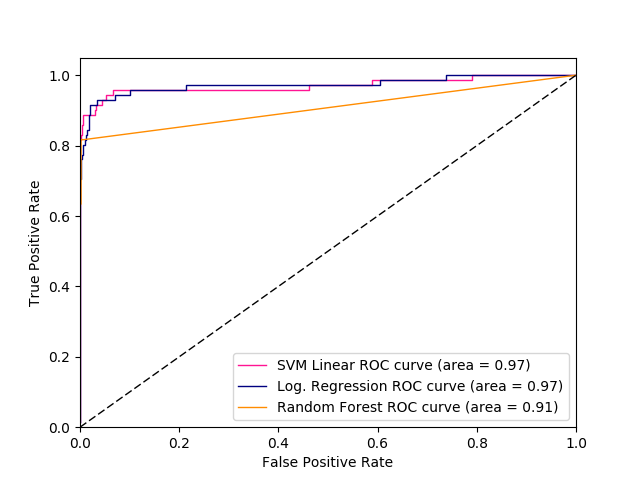
\includegraphics[width=0.7\textwidth]{figures/roc_auc_brazilian_travel_related}
  \label{fig:roc_curve}
\end{figure}

After the selection of our classification model, we decided to classify all the Portuguese dataset and draw some statistics from the results. The trained Linear SVM classifier was used to predict whether tweets were travel-related or not, since it was the model presenting the best score under the F1-score metric (as shown in Table~\ref{classifiers}). From a total of 7.8M tweets, our classifier was able identified 37,300 travel-related entries.

Fig.~\ref{predicted} depicts the distribution of travel-related tweets over the days of the week. We can see that the first three business days (Monday, Tuesday and Wednesday) are the ones on which the Twitter activity is higher for both cities in our study.

\begin{figure}[!htbp]
  \caption{Positive Predicted Tweets per Day of Week}
  \centering
    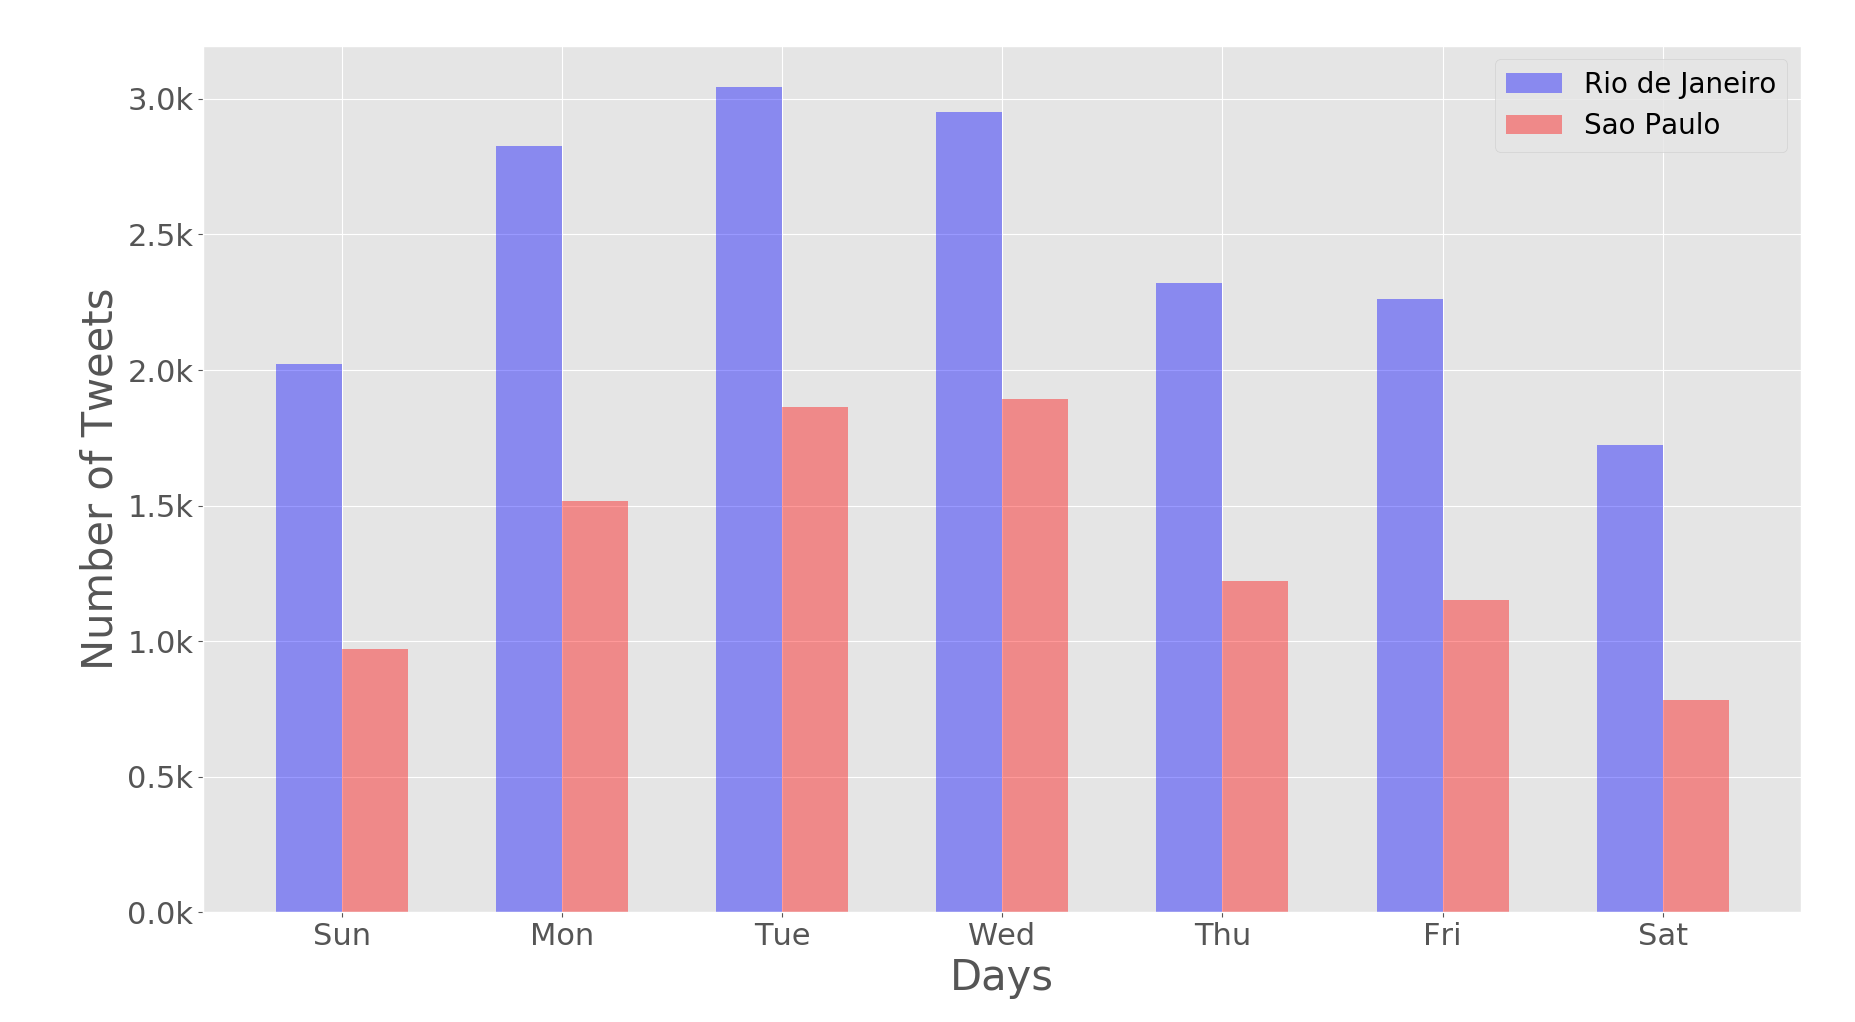
\includegraphics[width=0.7\textwidth]{figures/predicted_day_of_week}
    \label{predicted}
\end{figure}

\begin{figure}[!htbp]
  \caption{Rio de Janeiro Heatmap to the positive tweets}
  \centering
    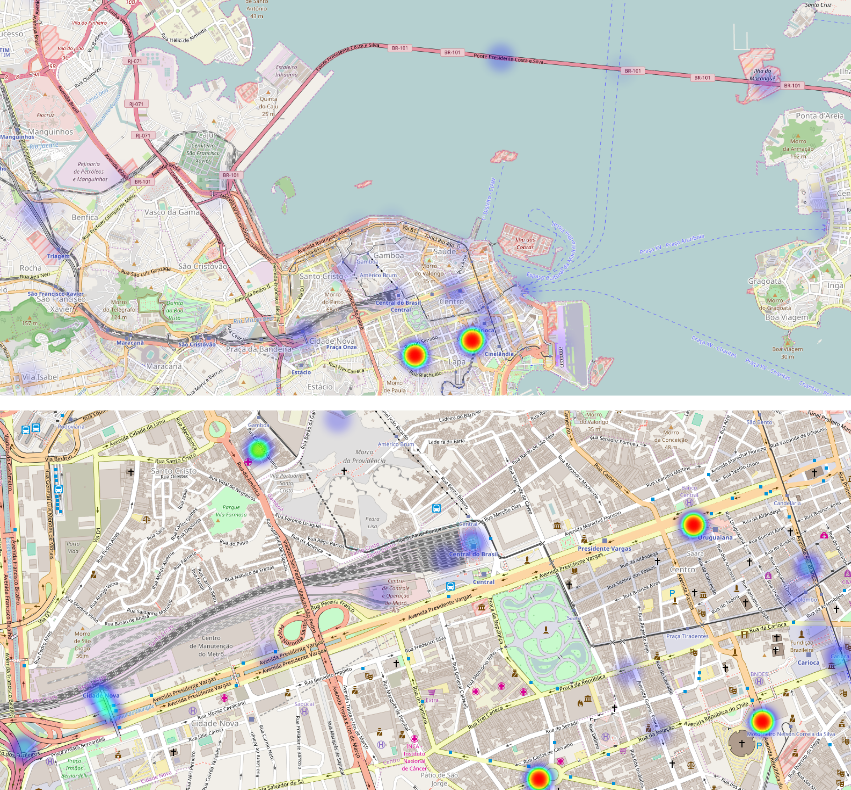
\includegraphics[width=0.725\textwidth]{figures/rio_1}
    \label{rio_heatmap}
\end{figure}

\begin{figure}[h]
  \caption{São Paulo Heatmap to the positive tweets}
  \centering
    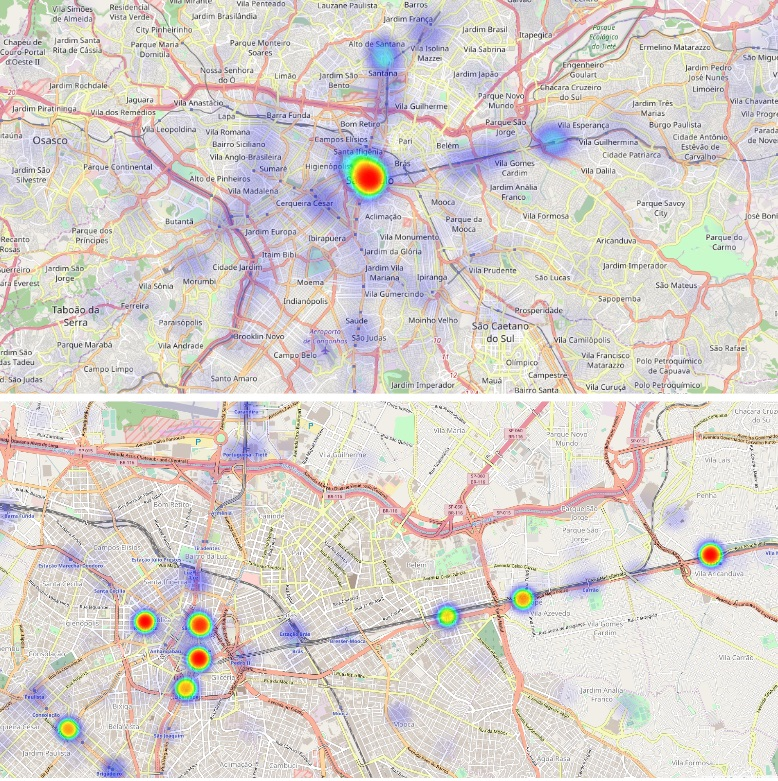
\includegraphics[width=0.725\textwidth]{figures/sp_1}
    \label{sp_heatmap}
\end{figure}

In order to understand the spatial distribution of travel-related tweets we generated a heatmap for both cities. From the heatmap of RJ, illustrated in Fig.~\ref{rio_heatmap}, it is possible to identify that some agglomerations of tweets are located at Central do Brasil, Cidade Nova and Triagem train stations, as well as at Uruguaiana, Maracanã and Carioca metro stations. The Rio-Niterói bridge, connecting Rio de Janeiro to Niterói, as well as the piers on both sides also presented considerable clouds of tweets classified as travel-related.

The heatmap for the city of SP, illustrated in Fig.~\ref{sp_heatmap}, was also an interesting case to observe. Almost every agglomeration matched some metro or train station. Estação Brás, Tatuapé, Belém, Estação Paulista, Sé, Liberdade were some of the stations highlighted in the heatmap. We could also identify a little agglomeration of travel-related tweets at Congonhas airport, even though no tweets seemed to mention the word \textit{plane} explicitly in the training of our classification model.

\subsection{Final Remarks}

\section{English Travel-related Classification}

Similar to the experiment of Portuguese travel-related classification, we built a model to discriminate english-speaking travel-related tweets. However, by following the same approach, final results were not improved with the combination of two different groups of features, bag-of-words and bag-of-embeddings.

The overall experiment steps as well as the final results are showed in the following subsections.

\subsection{Data Collection and Preparation}
Differently from the Portuguese experiment, tweets were collected from New York City during a period of two months, between days March 12 and May 12, 2017. Ignoring all non-English tweets the resulting dataset comprehends 4M tweets.

Regarding the preparation of data, we used the same preprocessing operations for each tweet present in our dataset:

\begin{itemize}
	\item \textbf{Lowercasing:} The message was converted to lowercase;
	\item \textbf{Transforming repeated characters:} Sequences of characters repeated more than three times were transformed, e.g. "sooooo" was converted to "sooo";
	\item \textbf{Cleaning:} Removing URLs and user mentions.
\end{itemize}

\subsection{Features Selection}
Two different types of features were defined to train our classification model, namely bag-of-words and bag-of-embeddings. Such groups are detailed below.

\begin{itemize}
	\item \textbf{Bag-of-words (BoW):} This type of features was obtained using unigrams with standard bag-of-words techniques. We considered the interval between 3,000 and 7,475 (maximum number obtained) of the most frequent terms across the training set excluding the ones found in more than 60$\%$ of the documents;
	
	\item \textbf{Bag-of-embeddings (BoE):} We applied bag-of-embeddings to each tweet using a \textit{doc2vec} model combining Deep Learning and \textit{paragraph2vec}. The model was trained with 10 iterations over the whole NYC dataset using a context window of value 2 and feature vectors with a size of 50, 100 and 200 dimensions. We then took the corresponding embedding matrix to yield the type of features fed into our classification routine.
\end{itemize}

\subsection{Training and Test Datasets}

The construction of the training and test sets were supported by the same term-based approach used in Section~\ref{subsec:training_test_datasets_portuguese} in order to filter tweets from the whole collection, i.e. we used the regular expression $space + term + space$ with each term presented in Table~\ref{tab:terms}. Firstly, 1,686 tweets were selected for each of both cases, travel-related and non-related. The travel-related set was strictly balanced in order to have almost the same amount of examples for each of the travel-modes involved in this study. The non-related training set is composed of several subjects that are not related to travel, e.g. football, leisure, politician, personal tweets, among others.

\subsection{Classification}
We choose a supervised learning approach in order to provide a robust solution for the classification task. Three learning algorithms were selected to conduct our experiments, namely Support Vector Machines (SVM), Logistic Regression (LR) and Random Forests (RF). The SVM classifier was tested under the \textit{linear} kernel function. To the LR classifier, standard parameters were applied, whereas the RF classifier was defined with 100 trees in the forest. The \textit{gini criterion} and the maximum number of features were limited to those as aforementioned in Section~\ref{features}, in the case of the RF classifier.
The performance of the resulting models will be compared in terms of \emph{precision}, \emph{recall} and the \emph{F1-score}.

\subsection{Preliminary Results}\label{subsec:preliminar_results}
In our first attempt, 10-fold cross-validation was applied for each model using, independently, bag-of-words and bag-of-embeddings as features. The results
showed us that all the models obtained good results regarding the selected evaluation metrics. The best model in this experiment was the Random Forests classifier trained with bag-of-words features, performing an F1-score of 0,977. Indeed, all the models that used bag-of-words features, in particular, revealed high scores as can be observed in Table~\ref{tab:first_experiment}. This may be explained by the similar vocabulary present in both training and test sets. One important note is that all travel-mode classes are known by the model before the classification of the test set. This may not be true in real-world scenarios. To further investigate the robustness of this features we designed another experiment that is explained in Section~\ref{subsec:leave_one_group_out}.

\begin{table}[htbp]
	\small
	\centering
	\caption{Preliminary Results}
	\label{tab:first_experiment}
	\begin{tabular}{|c|c|c|c|c|}
		\hline
		\textbf{Classifier} & \textbf{Features} & \textbf{Precision} & \textbf{Recall}  & \textbf{F1-score} \\ \hline
		\multirow{2}{*}{\textbf{Linear SVM}} & BoE (200) & 0,90883   & 0,83634 & 0,87089  \\
		& \textbf{BoW} & \textbf{0,96298}   & \textbf{0,97652} & \textbf{0,96962}  \\ \hline
		\multirow{2}{*}{\textbf{Logistic Regression}} & BoE (100) & 0,90172   & 0,84948 & 0,87447  \\
		& \textbf{BoW} & \textbf{0,96431}   & \textbf{0,98042} & \textbf{0,97222}  \\ \hline
		\multirow{2}{*}{\textbf{Random Forests}} & BoE (100) & 0,81283   & 0,83600 & 0,82394  \\
		& \textbf{BoW} & \textbf{0,96569}   & \textbf{0,98997} & \textbf{0,97764}  \\ \hline
	\end{tabular}
\end{table}

\subsection{\emph{Leave-one-group-out}}\label{subsec:leave_one_group_out}
The second experiment follows a \emph{leave-one-group-out} strategy. Meaning that one travel-mode class if left out of the training set and moved into the test set. This way, the behaviour of the learned model when facing a completely unknown travel-mode class can be evaluated.
A model for each hidden mode of transport class was built, and evaluation is carried as the previous experiment. The datasets composition of each experiment led in this strategy can be observed in Table~\ref{tab:leave}.

\begin{table}[htbp]
	\small
	\centering
	\caption{Datasets Composition}
	\label{tab:leave}
	\begin{tabular}{|c|c|c|c|c|}
		\hline
		\multirow{2}{*}{\textbf{\begin{tabular}[c]{@{}c@{}}Travel-Mode \\ Class\end{tabular}}} & \multicolumn{2}{c|}{\textbf{Training Set}} & \multicolumn{2}{c|}{\textbf{Test Set}} \\ \cline{2-5} & \textbf{Pos.} & \textbf{Neg.} & \textbf{Pos.}  & \textbf{Neg.}  \\ \hline
		Taxi & 1,372 & \multirow{6}{*}{1,686}   & 314 & \multirow{6}{*}{300}  \\
		Train & 1,369 & & 317 & \\
		Car  & 1,369 & & 317 & \\
		Bike & 1,386 & & 300 & \\
		Walk & 1,469 & & 217 & \\
		Bus  & 1,375 & & 311 & \\ \hline
	\end{tabular}
\end{table}

Each learning model experiment was made varying the hidden travel-mode class, which is unknown for our classifier in the training process. This method was performed in order to evaluate the sensitivity and robustness of the models built in our first experiment, described in Section~\ref{subsec:preliminar_results}. Table~\ref{tab:results} presents the best results for each model, as so its features and tuning parameters. The results from the models using bag-of-embeddings features revealed a consistent performance, i.e. they do not change even with the variation of the size of the feature vectors.

According to results, all classification models have performed reasonably well under the bag-of-embeddings features group, although the dimensionality used being different for the Linear SVM classifier.

\begin{table}[htbp]
	\small
	\centering
	\caption{\emph{Leave one group out} experiments results for SVM, LR and RF classifiers}
	\label{tab:results}
	\begin{tabular}{|c|c|c|c|c|}
		\hline
		\textbf{Classifier} & \textbf{Features}  & \textbf{Precision} & \textbf{Recall}  & \textbf{F1-score} \\ \hline
		\multirow{2}{*}{\textbf{Random Forests}} & BoW & 0,40774 & 0,07474 & 0,12629  \\
		& \textbf{BoE (50)}  & \textbf{0,80278} & \textbf{0,76194} & \textbf{0,78447}  \\ \hline
		\multirow{2}{*}{\textbf{Logistic Regression}} & BoW & 0,40774 & 0,07474 & 0,12629  \\
		& \textbf{BoE (50)}  & \textbf{0,84882} & \textbf{0,75702} & \textbf{0,80219}  \\ \hline
		\multirow{2}{*}{\textbf{Linear SVM}} & BoW & 0,41527 & 0,07153 & 0,12203  \\
		& \textbf{BoE (200)} & \textbf{0,86374} & \textbf{0,75715} & \textbf{0,81289}  \\ \hline
	\end{tabular}
\end{table}

\begin{figure}[!htbp]
	\centering
	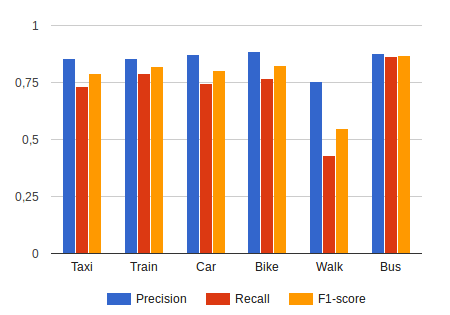
\includegraphics[scale=0.7]{figures/svm_linear_leave_one_out_emb_200.png}
	\caption{SVM model with BoE(200) for each travel mode}
	\label{fig:svm_leave}
\end{figure}

After testing each model with a hidden travel-mode class, the models trained with bag-of-words features demonstrated poor performance when facing unknown travel-modes, revealing higher sensitivity and lower generalization capabilities in comparison to the bag-of-embeddings version. The generalization power is an important and crucial characteristic for our desired solution. In a real world scenario is very likely that we will face a higher variety of categories that were not taken into consideration in the training phase of our model.

\begin{table}[htbp]
	\centering
	\small
	\caption{Sample of tweet messages correctly classified}
	\label{tab:tweets_examples}
	\begin{tabular}{|c|}
		\hline
		when you get into your uber and he has a pipe in the back \\
		a ground stop for \#ewr is no longer in effect \#flightdelay \\
		snowy walk to work. \#blizzard2017 \#centralpark \#noreaster2017 \@ bethesda terrace fountain -  \textbf{Figure~\ref{fig:central_park}} \\
		m.t.a. n.y.c subways: w train irregular subway service at whitehall street-south ferry \#traffic - \textbf{Figure~\ref{fig:brooklyn}} \\ \hline
	\end{tabular}
\end{table}

The best result of the \emph{leave-one-group-out} was the Linear SVM model, with the dimensionality of 200 in the size of the feature vectors. Figure~\ref{fig:svm_leave} presents the results of each experiment led for the different hidden travel-mode classes. An interesting point to observe is the low performance obtained to the experiment with the travel-mode class "Walk" hidden. This is due to the different semantic and syntactic contexts that the word \emph{walk} is used. Although all other classes can be used in the same context, for example, \emph{car}, \emph{train}, or \emph{bus}, usually the word \emph{walk} is not applied in the same way.

Having the experiments concluded, we used the best model, in this case, Linear SVM for the dimensionality of 200, to predict the 4M tweets that composed the NYC dataset. Almost 300,000 tweets were classified as travel-related. After the classification step, a sample of 10,000 tweets was taken from all the travel-related classified tweets and it was produced a heat-map distribution in order to verify which are the most concentrated zones. Such distribution enables the identification of associations with metro, train, bus stations. In Figure~\ref{fig:brooklyn}, that shows the south of the Manhattan island and also the Brooklyn bridge, it is possible no note some agglomerations over the bridge and also in the port and closed to the Wall Street(4.5) where there are some metro stations. The Central Park is one place that also took our attention since presented several agglomerations of tweets. In this particular place, tweets related to the walk class were correctly identified.

\begin{figure}[htbp]
	\centering
	\begin{subfigure}[htbp]{0.8\textwidth}
		\centering
		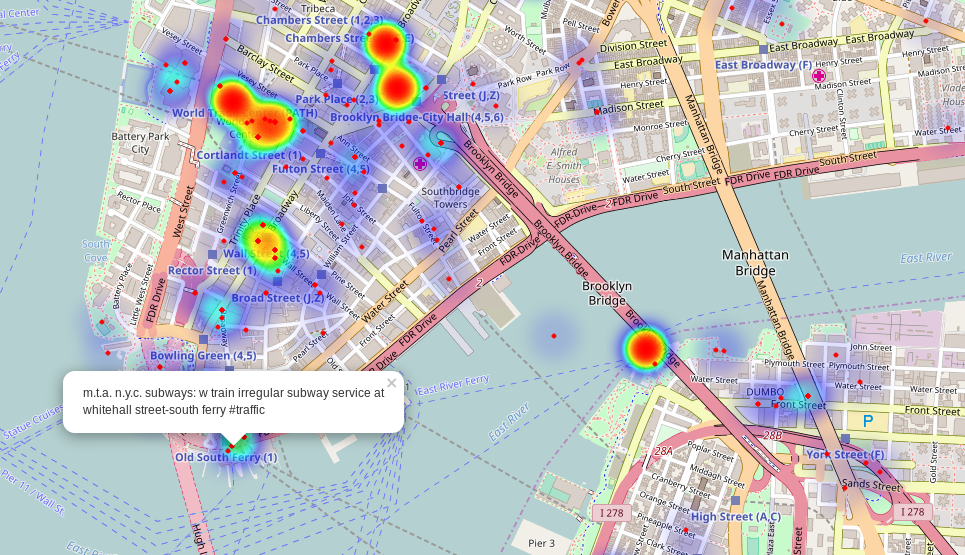
\includegraphics[width=0.9\columnwidth]{figures/nyc_map.png}
		\caption{}
		\label{fig:brooklyn}
	\end{subfigure}
	
	\medskip
	
	\centering
	\begin{subfigure}[htbp]{0.8\textwidth}
		\centering
		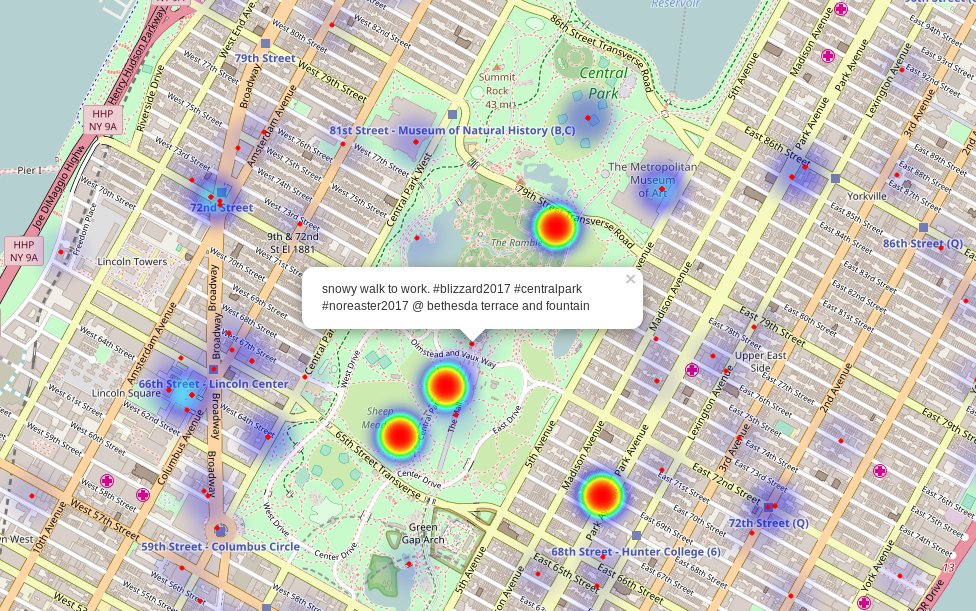
\includegraphics[width=0.9\columnwidth]{figures/nyc_map2.png}
		\caption{}
		\label{fig:central_park}
	\end{subfigure}
	
	\caption[Spatial density of the predicted tweets]{Spatial density of the travel-related predicted tweets in New York City: (a) South of Manhattan and over the Brooklyn Bridge, (b) Central Park}
	\label{fig:nyc_london_melbourne_geographical_distribution}
\end{figure}

\subsection{Final Remarks}

%\section{Travel-mode Extraction}\label{sec:travel_mode_extraction}
\section{Summary}
